\defcitealias{Eigenbrot16b}{Paper 2}
\defcitealias{Eigenbrot16a}{Paper 1}
\defcitealias{Mosby15}{M15}
\defcitealias{Bruzual03}{BC03}
\defcitealias{Maraston11}{MA11}

\chapter[NGC 891: Full Spectrum Analysis]{Vertical Population Gradients in NGC 891 II. Spectral Analysis}
\label{chap:891_2}
\epigraph{\fixspacing\emph{Science is magic that \underline{works}}}{Kurt Vonnegut}

\cleardoublepage

\begin{chabstract}

  We report the results of applying full-spectrum fitting methods to
  IFU data from NGC 891. The edge-on nature of this galaxy allows us
  to use line centroid velocity measurements to deproject on-sky radii
  to get a fully 3D picture of the location of our data in this
  galaxy. Our data are fit using a set of only 4 SSPs chosen, through
  statistical methods, to be a basis set for much larger SSP
  libraries. We attempt to refine the standard $\chi^2$ metric to make
  it more sensitive to spectral regions that encode information about
  age and metallicity, but find that this greatly increases
  uncertainty in our fits. Full spectral fits produce measurements of
  age, metallicity, and extinction as a function of height and radius
  in NGC 891. In this phase space we identify three key features: (i)
  a star forming disk below $|z| = \val{0.4}{kpc}$, (ii) a flared
  extension of this disk extending to $|z| = \val{1}{kpc}$ at radii
  beyond \val{8}{kpc}, and (iii) a high-metallicity sequence at large
  radii and large heights. We are also able to make rough estimates
  about the star formation history of NGC 891.

% We have determined the vertical population gradients in age and
% metallicity in the disk of NGC 891 based on optical spectroscopy.
% These gradients, measured over a range of projected radii, are
% combined with estimates of the dust attenuation as a function of
% radius and height. Using a parameterization of the radial population 
% gradients in the disk plane, we model the heating rate in this spiral
% disk and compare it to estimates in the Milky Way solar neighborhood.
% This abstract will get augmented as we consolidate our results and
% make decisions about how we undertake the analysis and what object to
% include. Here and in the following manuscript outline the text gives a
% description of possible content and analysis choices.  These should be
% viewed as suggestions to be edited and commented out or deleted as
% items are completed.


\end{chabstract}

\section{Introduction}

In Chapter \ref{chap:891_1} we used a focused set of spectral line
measurements to show that the signature of disk heating in NGC 891
matches observations of the Milky Way \citep[e.g.,][]{Bovy12,
  Hayden15} with startling accuracy. Near the midplane of NGC 891
($|z| < \val{0.4}{kpc}$) spectra have strong Balmer absorption
features, indicative of young stellar populations, while above
\val{0.4}{kpc} there is a sharp transition to spectra dominated by
metal abosportion, notably Ca H\&K, MgI, and Fe. Secondary results
include detection of a negative age gradient with radius, which could
be the signature of an inside-out formation history similar to that
seen in the Milky Way \citep{Bovy12, Hayden15}, and a potential flare
in the star-forming disk beyond \val{\asim 8}{kpc}.

{\bf MAB: In above paragraph I would say features associated Ca H\&K,
  the G band, Mgb and Fe bands 5270 and 5335.}

These results represent important new information about NGC 891 (and,
by extension, Milky Way-like disk galaxies), but they do not take
advantage of the full wealth of information contained in our
data. Specifically, the index measurements presented in
\ref{chap:891_1} consider each spectral feature in isolation
(or, at best, in relation to one other feature) and ignore the fact
that every spectral channel encodes information about the underlying
astrophysical pictures. By construction, the data taken by \GP and
described in \ref{chap:891_1} are of sufficiently high
signal-to-noise (S/N) that using the entire spectrum can yield
physical insights beyond what can be measured by line indices alone.

In this chapter I use full-spectral fitting to measure age,
metallicity, and extinction (our three ``quantities of interest'') as
a function of radius and height in NGC 891. As discussed in Chapter
\ref{chap:intro} full spectrum fitting requires an SSP basis set,
which in turn depends on stellar template library, IMF, and stellar
isochrones. In \S\ref{891_2:sec:SSP_sets} we explore a range of
different SSP libraries and ....
 
%% We choose to use the SSP templates of \citet{Bruzual03},
%% which are constructed with the Padova isochrones \citep{Bertelli94,
%%   Girardi00, Marigo08}, Chabrier IMF \citet{Chabrier03}, and STELIB
%% library \citep{LeBorgne03}.

%% The idea of using an
%% entire galaxy spectrum has a long history since \citet{Spinrad71}
%% first mixed stars together and modern techniques employ a variety of
%% sophisticated methods to extract the maximum about of data from each
%% wavelength. Regardless of specific method, all attempts at
%% full-spectrum fitting require the same basic ingredients: (i) a
%% library of stellar spectra, whether empirical or synthetic, (ii) a set
%% of isochrones that encapsulate how stars evolve with time, and (iii)
%% an initial mass function (IMF). With these three components
%% Astronomers can construct simple stellar populations (SSPs); a set of
%% stars of the same age and same metallicity/abundance with a mass
%% distribution determined by the IMF. To simulate an entire galaxy
%% multiple SSPs of different ages and metallicities are combine together
%% to produce a complext stellar population (CSP), which requires
%% assuming both a star formation history (SFH) and the
%% distribution/properties of dust in the galaxy. An excellent discussion
%% of this process can be found in \citet[especially his Figure
%%   1]{Conroy13}.

%% Within the general picture painted above there exists a wide range of
%% options and data. It is common for SSP libraries to be constructed
%% with the Padova isochrones \citep{Bertelli94, Girardi00, Marigo08}
%% because these models cover the widest range of stellar age and
%% chemical compositions, but other models are often used for their focus
%% on specific epochs of stellar evolution, for example high-mass stars
%% (Geneva \citep{Schaller92,Meynet00}), low-mass stars ($Y^2$
%% \citep{Yi01,Yi03}, or Dartmouth \citep{Dotter08}), and even very
%% low-mass stars (Lyon \citep{Chabrier97,Baraffe98}). In this work we
%% use exclusively the Padova isochrones because our observations, by
%% their very nature, light-weighted and therefore the specific details
%% of low mass stars are rather unimportant.

%% The choice of IMF can also affect the final modeled galaxy
%% spectrum. The canonical IMF of \citet{Salpeter55} was based on
%% observations of the Solar Cylinder in the Milky Way, and there is so
%% far little evidence that the IMF is appreciably different elsewhere in
%% the Universe \citep{Bastian10}. More recent observations have refined
%% the specific form of the IMF \citep{Kroupa01, Chabrier03}, but the
%% general picture remains the same. We use the IMF of \citet{Chabrier03}
%% because it is physically motivated and provides a good fit to low-mass
%% and brown dwarf star counts in the Milky Way
%% \citep{Bruzual03,Chabrier01,Chabrier03}.

%% Finally, the construction of SSPs depends on the stellar library
%% used. In this work we consider only empirical stellar libraries, and
%% more specifically on the STELIB \citep{LeBorgne03} and MILES
%% \citep{Sanchez-Blazquez06} libraries. The main strength of emperical
%% libraries is that the get the chemistry right by default, as indeed
%% they must. The cost of this accuracy, however, is a very limit
%% sampling of the entire parameter space of stellar evolution. For
%% example, as is discussed in \S\ref{891_2:sec:ma11}, the MILES library very
%% coarsly samples the metallicty/age plane and doesn't have any spectra
%% for ages below \val{6.5}{Myr}. We use the STELIB library because it
%% more finely samples stars of different ages, but warn that it still
%% lacks a detailed view of how spectra change with metallicity.

%% As discussed in \S\ref{891_2:sec:SSP_sets} we ultimately use the SSPs of
%% \citet{Bruzual03}, which are constructed with the Padova isochrones,
%% Chabrier IMF, and STELIB library. We note, however, that over the
%% wavelength range we consider ($\val{3800}{\AA} \leq\lambda\leq
%% \val{6800}{\AA}$) the differences in spectral shape caused by
%% different assumptions/models are minimal.

%% More directly relevant to our work is the assumption about the SFH
%% that is used to construct galaxies (CSPs) from SSPs. A common choice
%% for SFH is the so called $\tau$-model where the star formation rate
%% (SFR) follows an exponential function with a single scale parameter,
%% $\tau_\mathrm{SF}$. This analytic form is based on closed-box models
%% where the SFR depends linearly on gas density \citep{Schmidt59} and
%% offers an attractive, one parameter, parameterization of the SFH. In
%% this work we chose to use a non-parametric SFH (as discussed in
%% \S\ref{891_2:sec:SSP_method}) which allows us to reduce the systematics in
%% our results that arise from forcing the form of the SFR (systematics
%% are not completely eliminated, however, as discussed in
%% \S\ref{891_2:sec:sys_err}). Using this method results in a much larger set
%% of free parameters and puts more strain on the fitting code, but our
%% data have high enough signal to noise (\val{\asim 60}{\AA^{-1}}) to
%% make it a viable option.

%% Once model galaxies are constructed there are a multidue of methods
%% available to fit them to our data, for example those of
%% \citep{Cappellari04,Tojeiro07,Chen12,CidFernandes05,Ocvirk06,Wilkinson15,Sanchez16}. Regardless
%% of the method used these fits face the same common issues; namely how
%% to deal with known degeneracies between age, metallicity, and
%% extinction \citep{Oconnel76,Aaronson78,Worthey94,dePaz02}. In some
%% methods the extinction degeneracy can be mitigated by removing the
%% overall continuum from both the data and models before fitting
%% \citep[e.g.,][]{Ocvirk06,Wilkinson15} and then recovering an
%% extinction estimate either by measurements of gass emission (i.e., the
%% Balmer decrement) or separate analysis of the ``best fit'' galaxy
%% spectrum. Metallicity and age are more closely entwined and the
%% degeneracy between them more difficult to break. In this work we
%% attempt to quantify the uncertainties that arise from similarities
%% between SSPs that are degenerate with age and metallicity (see
%% \S\ref{891_2:sec:fit_err}), but note that we have not addressed systematic
%% uncertainties that may arise from our choice of model SSPs.

%% % {\bf Discussion of history
%% %   of SSP fitting}

%% % o PPXF (Cappelari 2004)
%% % o VESPA (Tojeiro 2007)
%% % o PCA (Chen 2012)
%% % o STARLIGHT (Cid Fernandes 2005)
%% % o STECKMAP (Ocvirk 2006)
%% % o FIREFLY (Wilkinson 2015?)

%% % {\bf MAB: History of SPS fitting is a big job. You might take a look
%% %   at Conroy's relatively recent ARAA article, and think about what you
%% %   want to focus on. One key issue is the move away from indices; this
%% %   is what folks have been doing for a while now. It might be worth
%% %   noting why we used indices in Paper I. The specific issues
%% %   associated with SPS and full spectral fitting (FSF) revolve around

%% % (1) completeness of stellar libraries;

%% % (2) stellar evolutionary tracks (isochrones), particularly for late
%% % phases of stellar evolution; and

%% % (3) fitting methods.

%% % Your task here should be to mention (1) and (2), and note that while
%% % you will be taking a look at two different set of libraries and tracks
%% % (BC03 and Maraston), in the wavelengths of interest there are not
%% % likely to be major differences. The more significant issue for you is
%% % in the fitting methods. Here I would further break this issue down 
%% % in terms of addressing the following question:

%% % How do codes handle the degeneracies in age and metallicity, and, more
%% % broadly, age, metallicity and extinction?

%% % We know about Firefly in terms of splitting off extinction. However,
%% % what is less clear is how various codes *pre*-select the set of
%% % templates to minimize degeneracy, and how they explore possible
%% % parameter space.  You are going to need to take some time to look at
%% % the literature on this. Pipe3D (Sebastian Sanchez); Starlight (Cid
%% % Fernandez); Vespa (Rita Tojeiro); and whatever Patricia Blazquez does.}

In addition to its importance as a nearby Milky Way analog, NGC 891
offers a unique perspective as one of the few galaxies close enough
for detailed study that is also perfectly edge-on. This orientation
allows for unambiguous measurements of vertical trends, but also
provides an opportuntiy to measure a fully three dimensional picture
of stellar populations. Unlike face-on disk galaxies, edge-on disk
galaxies have a clear and strong velocity structure along the line of
sight that is caused by the rotation of the galaxy. The detailed
kinematic structure of NGC 891 is known
\citep{Swaters97,Kregel05,Oosterloo07} and we can leverage this
knowledge to determine the true location of measured data within the
galaxy. In principle a detailed study of the kinematics (i.e., line
shape) of an edge-on galaxy like NGC 891 could yield a very detailed
picture of the that galaxy's line of sight (LOS) structure (what we
call ``doppler tomography''), but in this work we are restricted by
spectral resolution to simply measuring line centroids.

%+++++++++++++++++++++++++++++++++ {\bf MAB: I'd say more here about
% your preference for edge-ons for getting the 3D perspective. For
% example, the emission density profile (from stars or gas) along the
% line of sight, convolved with the velocity field, produces a line
% profile shape. This is what we mean by Doppler tomography; it
% requires some assumptions about the velocity field, which we take to
% be smooth and similar to the atomic gas, and about the smoothness of
% the density distribution of the emisssion, which was problematic for
% the ionized gas but probably a better bet for the older stars
% contributing to the metal-line absorption.  All that said, i.e., put
% out the idea, we use the line centroid only because of our limited
% resolution.}

The following paper is organized as follows: in \S\ref{891_2:sec:data} we
briefly describe the data of \ref{chap:891_1}, which is used
in this work. \S\ref{891_2:sec:anal} details further analysis needed to
ready the data for SSP fitting, along with our general fitting
methodology. In \S\ref{891_2:sec:LOS} we use velocity information to
determine the true, 3D location of our data in NGC 891, and in
\S\ref{891_2:sec:SSP_sets} we discuss a range of different SSP libraries and
motivate our final choice of library used for fitting. An attempt to
improve the precision of our fits by modifying $\chi^2$ is shown in
\S\ref{891_2:sec:smart_chi} while in \S\ref{891_2:sec:uncertainty} we quantify
both fitting and systematic uncertainties present in our
analysis. Finally, \S\ref{891_2:sec:results} presents a new view of the
phase-space of NGC 891 as revealed through our full spectrum fits and
we summarize this work in \S\ref{891_2:sec:summary}.


\section{Data}
\label{891_2:sec:data}
The data used in this paper were recorded using \GP \citep{Wood12} on
the WIYN\footnote{The WIYN Observatory is a join facility of the
  University of Wisconsin-Madison, Indiana University, NASA, and the
  National Optical Astronomy Observatory.} telescope Bench
Spectrograph \citep{Barden94,Bershady08,Knezek10}. In Chapter
\ref{chap:891_1} we detail the observational methodology, data
reduction, and spectral coadding used to produce the spectra that will
be used in this work. Briefly, spectra were extracted and reduced
primarily using standard IRAF tasks with some custom modifications to
account for the unique nature of \GP. The individual fibers were then
coadded to produce ``aperture'' spectra that have signal to noise
$\geq \val{30}{px^{-1}}$ (\val{\asim 20}{\AA^{-1}}). We refer the
reader to Chapter \ref{chap:891_1} and Appendix
\ref{chap:full_ap_table} for an in-depth discussion of all of these
steps and tables listing the details of each aperture (location,
constituent fibers, etc.).


\section{Basic Analysis}
\label{891_2:sec:anal}

To quantify uncertainties in our full spectrum fitting methods we will
test different methods of fitting spectra and interpreting the
results. In this section we describe the basic, high-level methodology
that is common to all fitting methods. We also detail prepatory
analysis that is required before these methods can be applied to our
data, namely determining the velocity of each aperture and correcting
for Balmer emission.

%+++++++++++++++++++++++++++
%% {\bf MAB: Itemize (not in bullets, in sentences, clauses) the detailed
%%   preparatory analysis you will be describing. ``running the data
%%   through full spectrum fitting'' should be re-worded.

%------------------------
%% You should also have some preliminary discussion about why you are
%% laying the basics on the ``SSP fitting methodology.'' (I would call it
%% SPS not SSP, i.e., your SPS involves adding together SSPs.) For
%% example, there are the issues of degeneracies between age, metallicity
%% and extinction. There is also the issue of assumptions about the SFH
%% on $\tau_L$ and $Z_L$ for which the data cannot offer resolution,
%% i.e., the data does not allow you to know about the detailed SFH for
%% the older stellar populations. In other words, what is going to lead
%% you ultimately to the DFK approach. Foreshadow this.}

\subsection{SSP fitting methodology}
\label{891_2:sec:SSP_method}

Our fitting method involves minimizing differences between measured
NGC 891 spectra and synthetic galaxy spectra constructed from the
superposition of simple stellar populations (SSPs, see
\S\ref{891_2:sec:SSP_sets}). Fits are performed with
MPFITFUN\footnote{available at \url{http://purl.com/net/mpfit}}
\citep{Markwardt09}, an IDL implementation of the MINPACK Levenberg
Marquardt minimization algorithm \citep{More78}. The model galaxy
spectra are defined as
\begin{equation}
\label{891_2:eq:SSP_galaxy}
g(\lambda) = R(\lambda,\tau_V) \sum_{i,j} M(\Delta t_i,Z_j)
f(\lambda,\Delta t_i, Z_j),
\end{equation}
where $f(\lambda, \Delta t_i, Z_j)$ is the spectrum of an SSP with
metallicity $Z_j$ formed over time interval $\Delta t_i$, $M(\Delta
t_i,Z_j)$ quantifies the strength of the contribution of each SSP, and
$R(\lambda, \tau_V)$ governs the total extinction in the galaxy. All of our
SSPs are normalized to \val{1}{\sol{M}} so the strength of each SSP is
simply
\begin{equation}
\label{891_2:eq:fit_weight}
M(\Delta t_i,Z_j) = \int_{\Delta t_i} \psi(t, Z_j) dt,
\end{equation}
where $\psi(t, Z_j)$ describes the mass of stars formed at time $t$
with metallicity $Z_j$ (i.e., the star formation rate). In other
words, $M(\Delta t_i,Z_j)$ is the total mass in stars formed during
the time interval, $\Delta t_i$, associated with a particular SSP. The
extinction $R(\lambda, \tau_V)$ is parametrized by a single variable,
$\tau_V$ and, importantly, does not depend on SSP age ($t_i$) or
metallicity ($Z_j$). In \S\ref{891_2:sec:extinction} we discuss the details
of $R(\lambda, \tau_V)$ and the limitations of this
simplification. During fitting the free parameters are the SSP
weights, $M(\Delta t_i,Z_j)$, a single extinction term, \tauV, and the
systematic velocity.

%+++++++++++++++++++++++++++++
%% {\bf MAB: You should reference Levenberg Marquardt but I do not think
%%   you need to describe your coding language or the implementation in
%%   MPFITFUN. Concerning equation (1), you need to mention here what is
%%   being assumed given the placement of R. You can discuss it more
%%   later (in 3.3), but you should at least note the implications here
%%   and point to that later discussion here.}

For each aperture our primary values of interest are the age,
metallicity, and extinction. We measure extinction directly as $A_V =
1.086\ \tauV$, but age and metallicity depend on assumptions made
during fitting (i.e., priors in the SSP library) and during subsequent
analysis.

As shown in Equation \ref{891_2:eq:fit_weight} the fit weights describe the
integral of a particular star formation history (SFH), but it is
useful to reduce a SFH down to single values for age and
metallicity. To do this we define a pair of light-weighted
quantities. The mean, light-weighted age is
\begin{equation}
\label{891_2:eq:MLWA}
\tau_L = \frac{\sum_{i,j} W_{L,i,j}\times t_i}{\sum_{i,j} W_{L,i,j}}
\end{equation}
where $t_i$ is the age associated with each SSP and $W_L$ is the
``light weight'', defined as
\begin{equation}
\label{891_2:eq:light_weight}
W_{L,i,j} = M(\Delta t_i,Z_j)\sum_k S(\lambda_k) R(\lambda_k, \tau_V)
f(\lambda_k, \Delta t_i, Z_j),
\end{equation}
where $S(\lambda_k)$ defines a bandpass over which the light weight is
computed. We set $S(\lambda_k)$ to be flat over \val{5450}{\AA}
$\leq\lambda\leq$ \val{5550}{\AA} and zero everywhere else. The choice
of $t_i$ depends on assumptions about the SFH and in this work we make
the simple assumption that star formation is constant across the
lifetime of each SSP ($\Delta t_i$) so that $t_i$ is simply the
midpoint of each $\Delta t_i$. In \S\ref{891_2:sec:sys_err} we discuss and
quantify the systematics that arise from such an assumption. Similarly
to $\tau_L$ we also define the mean, light-weighted metallicity as
\begin{equation}
\label{891_2:eq:MLWZ}
Z_L = \frac{\sum_{i,j} W_{L,i,j}\times Z_j}{\sum_{i,j} W_{L,i,j}}.
\end{equation}

We note that Equation \ref{891_2:eq:light_weight} also describes a
conversion from mass-weights (i.e., $M(\Delta t_i, Z_j)$) to
light-weights that is simply a constant that is independent of the
specific mix of SSPs (but does depend on the overall extinction).

%+++++++++++++++++++++++
%% {\bf MAB: In eqn (4) move M outside of the sum since it does not
%%   depend on wavelength to clearly indicate that the factor between the
%%   light weight and the mass (weight) is a contant factor that depends
%%   on age and metallicity for a given band-pass. And say as much.}

\subsection{Velocities}
\label{891_2:sec:vel}

\begin{figure*}[t]
  \centering
  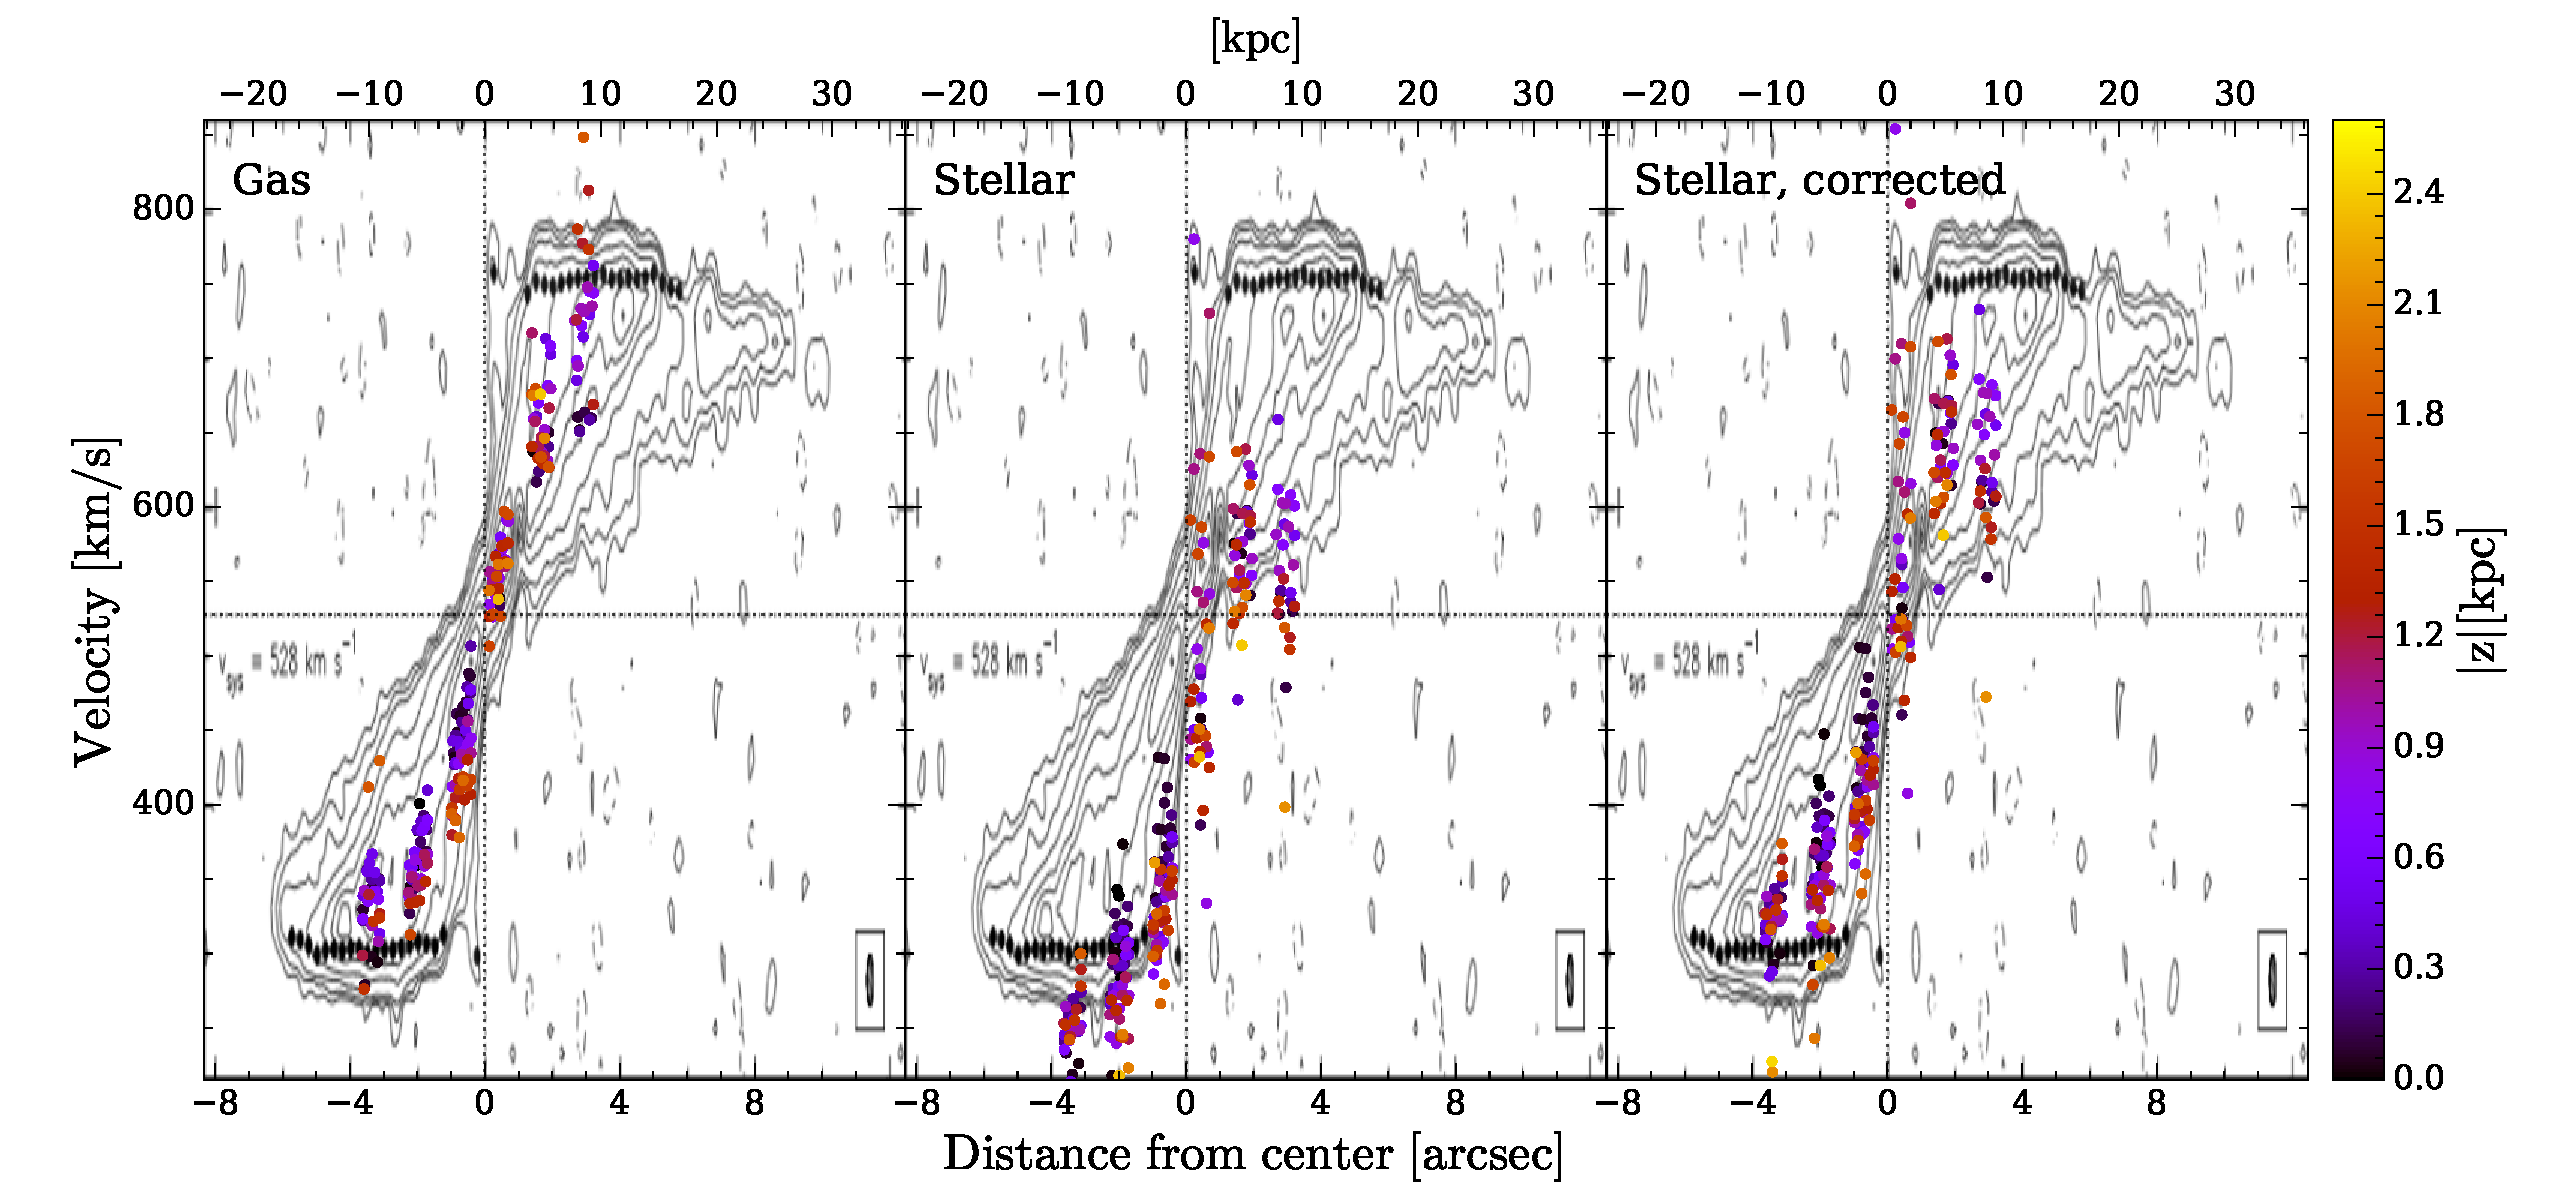
\includegraphics[width=\textwidth]{891_2/figs/Swat_vel.pdf}
  \caption[Comparison of measure stellar and gas velocities to HI
    velocity data]{\fixspacing\label{891_2:fig:Swat_vel}Comparison of
    HI velocity envelope (from \citet{Swaters97}) to \emph{left:}
    measured H$\alpha$ centroids, \emph{middle:} best fit velocities
    from SSP models, and \emph{right:} best fit stellar velocities
    with a constant offset to minimize median difference between gas
    and stars.}
\end{figure*}
The systemtic velocities of our model spectra do not depend on the
shape of the spectra (i.e., the SSP mix) and thus we can reduce the
number of free parameters in our SSP fits by measuring the velocities
once and then keeping them fixed for all subsequent analysis. The
final velocity values are a combination of velocity estimates from two
sources: the ``fit'' velocities that result from SSP fitting, and
velocities measured from the centers of bright emission lines.

%++++++++++++++++++++++
%% {\bf MAB: Do you mean ``systematic velocities'' or do you mean
%%   ``systemic velocities'' or ``line of sight velocities'' ? At the end
%%   of the paragraph enumerate in words what the following two
%%   subsubsections are.}

\subsubsection{Fit velocities}
During full spectrum fitting the velocity can be a free parameter of
the model, and this fit provides the first estimate of the velocity of
each aperture. The first step is to run a fully unconstrained fit
where all SSP weights, the velocity, and the extinction are allowed to
vary (see \S\ref{891_2:sec:SSP_method}. This produces a ``best fit'' only in
the sense that the resulting model spectrum matches the data well in a
$\chi^2$ sense; to determine velocities the details of the
astrophysical assumptions behind each model are unimportant. The
velocities found during fitting are generally precise on the order of
\val{\asim10}{\kms}, depending on \GP fiber size (see
\ref{chap:891_1}), which is slightly better that 10\% of the
instrumental resolution (again, depending on fiber size).

%++++++++++++++++++
%% {\bf MAB: Discuss the centroiding accuracy in terms of the
%%   instrumental resolution.}

Once the ``best fit'' spectrum is determined we run a second iteration
of the fitting routine with the SSP weights and extinction fixed to
the best fit values. This keeps the shape of the model spectrum the
same and causes $\chi^2$ minimization to be driven only by the
velocity offset between the model and the data. When fitting these
velocities we used only the range of wavelengths that lie within the
region spanned by arc lamp lines ($\val{4100}{\AA} \leq\lambda\leq
\val{6600}{\AA}$). This avoids wavelengths that could be affected by
extrapolation of the wavelength solution (see
\ref{chap:891_1}). In the majority of apertures this
``refined'' velocity was within \val{\asim 10}{\kms}, which is similar
to the precision of the fits and indicates that this second iteration
is perhaps not necessary.

%+++++++++++++++=
%% {\bf MAB: How important is this iteration? Again, compare amplitude of
%%   the change in the iteration to the instrumental resolution.
%% Refer to Paper-I concerning the wavelengths spanned by arcs (at the end of
%% the last sentence of the par.
%% }

The results of these fits produce what we call the ``fit
velocities''. The final fit values were found to be stable to a wide
(\val{\asim 100}{\kms}) range of starting velocity values. These
velocity fits are driven mainly by regions of the spectrum that
deviate significantly from the continuum level, which in our case are
the Balmer absorption series, the MgI absorption band, and the G
band. Many apertures show moderate to strong \Ha emission, but we
masked this feature (and [OIII]) during fits because our model SSPs do
not have nebular emission. For this reason the $\chi^2$ velocities can
be though of as the ``stellar'' velocity values.

%% {\bf MAB: Do you mask the upper Balmer series, including H-beta? I
%%   would have thought this would be important, and I thought you did.}

%% Comment for MAB: we actually didn't mask \HB. In retrospect maybe we
%% should have, but it is a rare aperture indeed that has strong enough
%% \HB emission to really mess with the residuals. Besides, the other
%% strong absorption features are certainly enough to simply fit a
%% centroid.

\subsubsection{Emission line velocities}

As a check on the velocities found above we also measure the velocity
of nebular emission lines, namely \Ha. Centroids were computed using
the IRAF task FITPROFS which allows us to deblend the \Ha, [NII]
complex. We focus only on the \Ha velocities, which are then compared
to known HI velocities from \citet{Swaters97}, as shown in the left
panel of Figure \ref{891_2:fig:Swat_vel}. We call the velocities measured in
\Ha ``gas velocities''.

%+++++++++++++++=
%% {\bf MAB: While I am ok with us comparing to Swaters+97 in Figure 1,
%%   are you taking into account in all of this analysis the trend in the
%%   HI tangential speed with height found in Oosterloo+07? This is
%%   essential I think. Last sentence are you measuring \Ha velocities or
%%   \Ha+[NII] velocities?}

The center panel of Figure \ref{891_2:fig:Swat_vel} shows the ``stellar
velocities'' compared to known HI velocities and our measured \Ha
velocities. Clearly there is a systematic offset between the stellar
and gas velocities that is relatively constant across both sides of
the galaxy. We find that this offset is constant in magnitude and sign
across both sides of the galaxy. This fact rules out an offset caused
by asymmetric drift \citep{Binney87}. Furthermore, many of the stellar
velocities are unphysical in the sense that they lie outside of the HI
envelope. We therefore conclude that this offset is caused by
systematic measurement uncertainty (likely arising from uncertainty in
our wavelength solution) and compute a constant velocity ``correction''
that is applied to the stellar velocities. This offset is computed to
minimize the median difference between stellar and gas
velocities. While we expect the stellar tangential speed to lag behind
the gas since we measure both sides of the galaxy, the median
difference between gas and stars should be, to first order, zero.

%+++++++++++++++++++++
%% {\bf MAB: I made a few edits in the above par. As part of or before
%%   the sentence beginning ``Clearly, ...'', add a description of what
%%   you see in Figure 1 that is clearly unphysical, i.e., the negative
%%   velocities in the middle panel below the gas. More broadly, discuss
%%   first the distribubtion of the ionized gas velocity w.r.t. the
%%   envelop from HI. This envelop should be noted in the text and the
%%   figure caption. Explain why we might expect the ionized gas to lie
%%   below the HI envelop, i.e., we are measuring a centroid. What should
%%   the reader make of the few points in the upper part of the left
%%   panel that are above the HI envelope? Are these bad measuremets? Add
%%   error bars?

%%   Define AD -- you can reference Binney \& Tremaine.

%%   Discuss what the soures of possible uncertainty could be in the
%%   stellar velocities. Is this a problem with the wavelength solution
%%   -- something that you come to in the next paragraph, or something
%%   else? Did you check that the wavelength solution and the BC03
%%   templates were either both in vacuum or air?

%---------------------
%%   Lastly, concerning the use of the median, yes, maybe to to zeroth
%%   order the median difference should be zero, but not to a \kms
%%   level. The median difference is going to depend on at least the
%%   number of points on the positive and negative sides of the galazy to
%%   zeroth order. To first order it will depend on the radial
%%   distribution particularly near the center where the projected
%%   velocity is small. Can you address this?}

\begin{figure}[t]
  \centering
  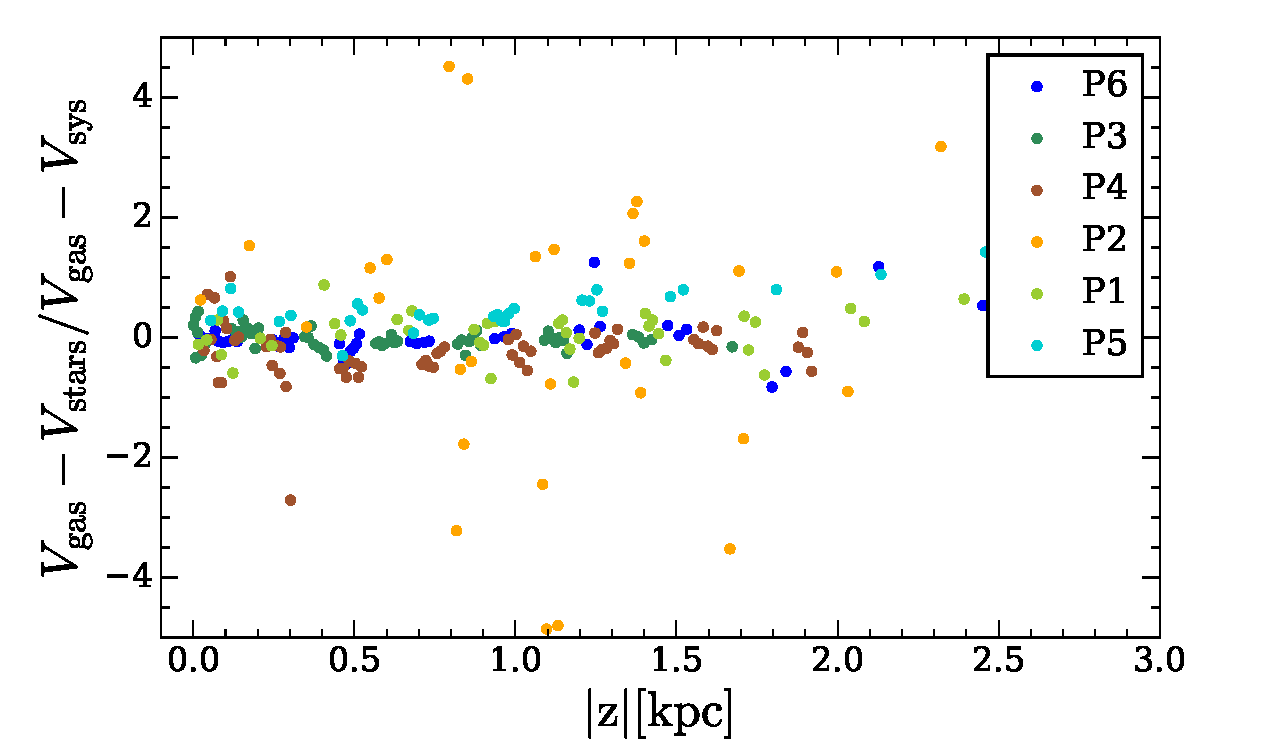
\includegraphics[width=\columnwidth]{891_2/figs/SG_diff.pdf}
  \caption[Offset between stellar and gas
    velocities]{\fixspacing\label{891_2:fig:SG_offset}Difference
    between stellar and gas velocities after applying a constant
    \val{74}{\kms} offset to the stars. A median of 1 corresponds to
    no average offset between the two population \emph{across both
      sides of the galaxy}.}
\end{figure}

Figure \ref{891_2:fig:SG_offset} shows the relation between stellar and gas
velocities after applying an offset of \val{74}{\kms}. Based on these
results, the final velocity of each aperture is fixed as the velocity
measured during $\chi^2$ fitting (``stellar velocity'') plus a
constant offset of \val{74}{\kms}. The right hand panel of Figure
\ref{891_2:fig:Swat_vel} shows the final velocities used. We note that the
systematic correction of \val{74}{\kms} is within the total
uncertainty in our velocity as dictated by uncertainties in the
wavelength solution (\val{120}{\kms}, see \ref{chap:891_1}).

%+++++++++++++++++++=
%% {\bf MAB: The standard is km s$^{-1}$ not \kms. At the end here you
%%   want to discuss the difference between the stars and gas in the left
%%   and right panels compared to each other and the HI envelop. For
%%   example, the asymmetry in the stars is not seen in the gas.}

\subsection{Extinction Model}
\label{891_2:sec:extinction}

During full spectral fitting (\S\ref{891_2:sec:SSP_method}) we assume the
extinction model of \citet{Charlot00} during all analysis steps, which
is described by
\begin{equation}
R(\lambda) = e^{-\tauV \left(\lambda/\val{5500}{\AA}\right)^{-0.7}}.
\end{equation}
This model has a steeper slope than a simple foreground dust screen,
but the authors show it accurately reproduces the ratio of
far-infrared to ultraviolet luminosities, the ratio of \Ha to \HB
luminosities, the \Ha equivalent width, and the ultraviolet spectral
slope of nearby starburst galaxies. We retain the functional
dependence of $\tau \propto \lambda^{-0.7}$ and define two
normalizations, one for gas emission and one for stellar
continuum. Thus, the total optical depth to a particular species is
either
\begin{equation}
\tau_{{\rm cont}}(\lambda) = \tauV \left(\frac{\lambda}{\val{5500}{\AA}}\right)^{-0.7}
\end{equation}
or
\begin{equation}
\label{891_2:eq:tauVB}
\tau_{{\rm em}}(\lambda) = \tauVB \left(\frac{\lambda}{\val{5500}{\AA}}\right)^{-0.7},
\end{equation}
where \tauV and \tauVB are the normalization factors for stellar continuum and
gas emission, respectively.

As described in \S\ref{891_2:sec:SSP_method}, \tauV is a free parameter of
the SSP models that essentially measures the slope of the
continuum. To measure \tauVB we use the ratio of measured \Ha/\HB flux
and compare it to the expected value of 2.86 from
\citet{Osterbrock89}, assuming case B recombination in a \val{10^4}{K}
gas. Under these assumptions, and given the extinction law in equation
\ref{891_2:eq:tauVB}, we compute
\begin{equation}
\label{891_2:eq:Balmer_extinction}
\tauVB = 4.84 \ln \left(\frac{\Ha/\HB}{2.86}\right).
\end{equation}

The \Ha and \HB line fluxes were measured using the IRAF task FITPROFS
which allows us to deblend the \Ha/[NII] emission feature. Before
fitting the emission lines a ``best fit'' galaxy model is
subtracted. As in \S\ref{891_2:sec:vel} the detailed astrophysics of the
best fit model are unimportant; we only require that the model
accurately match the stellar continuum so that it can be subtracted
from the data. Once the continuum is subtracted the data are smoothed
with a 3 pixel (\val{\asim 350}{\kms}) wide moving average. To
mitigate the impact of bad continuum fits the centroid fitting window
is constrained to be only $\sim 4\sigma$ wide, where $\sigma$ is the
average spectral width (standard deviation) of bright sky emission
lines.

%++++++++++++++++++==
%% {\bf MAB: In the first sentence above do you mean SSP or SPS? I think
%%   the latter. Concerning the 600 \kms wide moving average, is this
%%   equivalent to a boxcar of xx pixels? If so, you might say ``the data
%%   are smoothed with a 600 km s$^{-1}$ (XX pixel) wide moving average,
%%   or boxcar.'' Again, modify \kms to km s$^{-1}$. However, I am not
%%   sure I understand the need for this smoothing and how it reduces the
%%   impact of bad continuum fits. Why? It seems to me you will make the
%%   NII+Ha blending worse which also sounds like it is a problem.}

The relative strength of the two [NII] lines in the \Ha/[NII] complex
is governed by quantum mechanics and we expect the flux ratio
[NII]$_{6585}$/[NII]$_{6549} = 3$. When measuring the \Ha/[NII] lines,
however, we often find [NII]$_{6585}$/[NII]$_{6549} > 3$, which
indicates that the line fit is attributing some of the [NII]$_{6549}$
flux to \Ha and causing the \Ha flux to be overestimated.  This is
likely due to an incorrect de-blending of the \Ha and [NII]$_{6549}$
lines.  We correct for this effect by using the flux of [NII]$_{6585}$
as a ``calibration'' flux (reasonable given its isolation, away from
blending issues of \Ha and [NII]$_{6549}$) and define an \Ha
correction,
\begin{equation}
  \label{891_2:eq:balmer_corr}
  \Delta\Ha = \mathrm{[NII]}_{6549} - \frac{\mathrm{[NII]}_{6585}}{3},
\end{equation}
which is added to the measured \Ha flux.

As mentioned above, measuring \Ha and \HB emission requires first correcting
for \Ha and \HB absorption present in the stellar continuum. In practice the
entire process is iterative because fitting SSPs accurately requires accurate
emission corrections (\S\ref{891_2:sec:emission_corr}), which, in turn, requires
accurate extinction values. We find that the measured Balmer fluxes
and derived emission corrections are stable after only a single
iteration.

%+++++++++++++++
%% {\bf MAB: I would like to understand the issue with the imperfect
%%   continuum subtraction (in the sentence ``This is likely due...'')
%%   and how it alters the NII ratio. In this paragraph, leading up to
%%   the motivation for eqn 10 you want to say that the concept here is
%%   to trust the 6585 NII line because of its greater wavelength
%%   separation from Ha. However, you also need to address wy you think
%%   the continuum subtraction is better for 6585, i.e., why for some
%%   reason the baseline for this line isn't what is causing the problems
%%   with the ratio not equalling 3. 

%-----------------
%%   Further, you need to provide the
%%   amplitude of the correction which I expect will vary significatly
%%   with Ha line-strength and height (NII/Ha changes). So I'd like to
%%   know the \% correction to the Ha flux in the mean (and/or median),
%%   and the trends with height, e.g., numbers for 0-0.4 kpc, 0.4-1 kpc,
%%   $>$1 kpc.}

\subsection{Emission Corrections}
\label{891_2:sec:emission_corr}

Many of our apertures show moderate to strong Balmer emission that is
not present in the SSP libraries that underlie our galaxy models and
therefore must be subtracted before accurate analyses can be made. To
do this we construct a model spectrum containing only emission from
\Ha, \HB, \Hg, \Hd, and \He.  The basic idea is to first construct a
model galaxy based on fits that mask the cores of the Balmer lines and
then use these fits to remove the stellar continuum and isolate the
Balmer emission. Then the two strongest emission lines (\Ha and \HB)
can be used to construct a model containing emission from the
higher-order lines.  Based on the results of \citet{Osterbrock89}, and
assuming case B recombination in a \val{10^4}{K} gas, the ratios of
fluxes for the Balmer series is \mbox{1 : 0.350 : 0.164 : 0.087 :
  0.056} (\Ha : \HB : \Hg : \Hd : \He). In our emission models the
width of each line is dictated by the instrumental resolution measured
at the line location (see \ref{chap:891_1}), with apertures
made from different sized \GP fibers having different widths.

%++++++++++++++++++++=
%% {\bf MAB: First sentence: I think you mean SPS models (that use
%%   SSPs). I'd like you to explain the notion behind the approach in an
%%   explicit way. The notion is an important idea. The kernel of it is
%%   that Hydrogen Balmer Case B emission strength decreases sigificantly
%%   with higher order, e.g., by more than a factor of 10 between
%%   H$\alpha$ and H$\delta$. In contrast, the equivalent width of the
%%   Hydrogen Balmer absorption in stellar photospheres does not display
%%   this trend, and indeed H$\alpha$ absorption EW is weaker than
%%   H$\beta$. This contrast can be used to our advantage in an iterative
%%   scheme that first masks the cores of the Balmer absorption lines
%%   where the emission is present to provide a first-order estimate the
%%   continuuum. Once subtracted, only the two strongest emission lines
%%   are used to estimate the normalization of the emission and the
%%   attenuation, from which the remaining line-emission is estimated.}

\begin{figure}
  \centering
  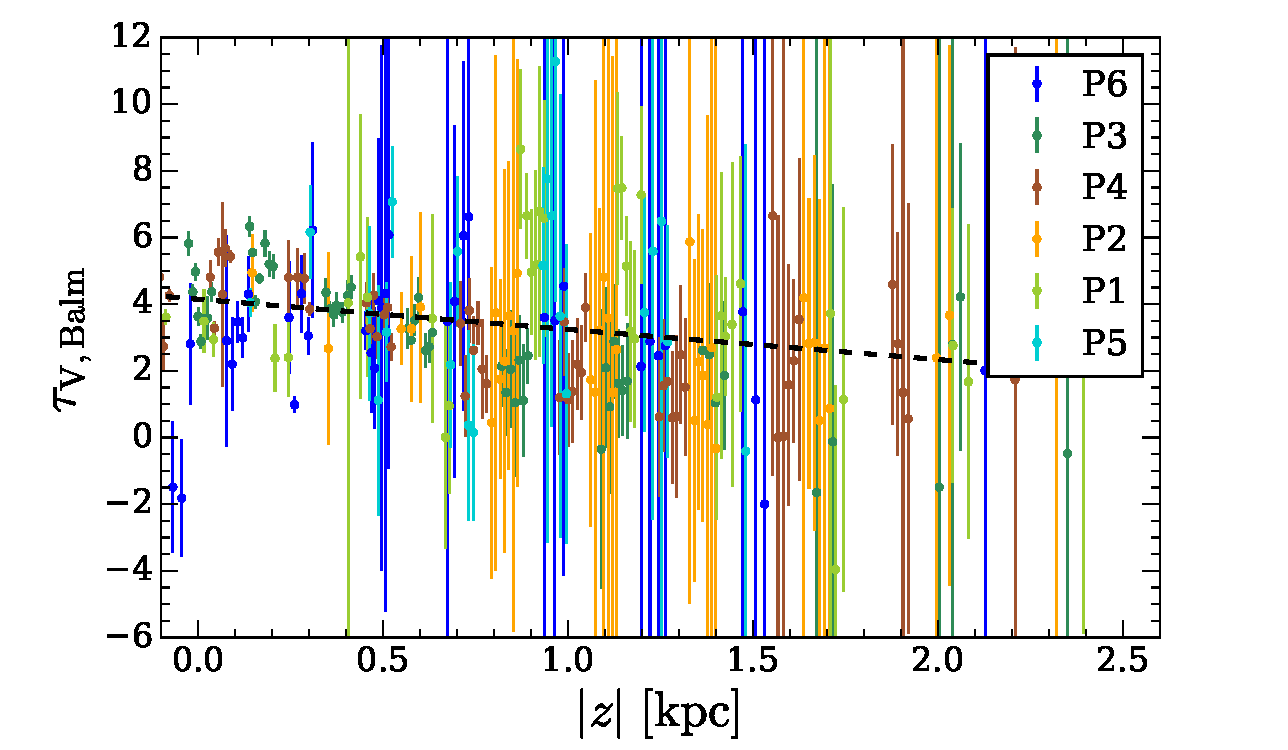
\includegraphics[width=\columnwidth]{891_2/figs/TauV_balm.pdf}
  \caption[Height dependendence of
    \tauVB]{\fixspacing\label{891_2:fig:tauVB_height}Measured values
    of \tauVB as a function of distance from the midplane. The error
    bars show the uncertainties reported by IRAF from 100 Monte Carlo
    noise iterations. The black shows a linear fit described in
    Equation \ref{891_2:eq:tauVbalm}.}
\end{figure}

This idealized Balmer emission model is then extincted using Equation
\ref{891_2:eq:Balmer_extinction} based on the value of \tauVB as measured in
section \ref{891_2:sec:extinction}. To minimize the impact of aberrant
extinction calculations we compute a height-dependent \tauVB by
fitting a line to the data from all apertures (and thus from all
radii), as shown in Figure \ref{891_2:fig:tauVB_height}. From these data it
is clear that the radial dependence to the vertical trend in \tauVB is
minimal so our grouping of all radii is valid. We find for NGC 891
\begin{equation}
\label{891_2:eq:tauVbalm}
  \tauVB (z) = -0.91 z + 4.15,
\end{equation}
which allows us to compute the extinction in our Balmer emission
models at any height above the midplane.

%----------------------
%% {\bf MAB: Concerning Figure 3: Yuck. I can't tell if the line is a
%%   good fit to the data and whether there is a radial dependence. (You
%%   should say ``a radial dependence to the vertical trend.'') Clearly
%%   we see a radial trend in the stellar absorption later so this result
%%   is somewhat puzzling without some thought and
%%   interpretation. Regarding the figure itself, I'd like to see a
%%   version w/o the error bars. The error bars must be wrong because
%%   they are far larger than the scatter. I would also like to see
%%   moving averages for all pointings as well as for individual
%%   pointings.}

\begin{figure}
  \centering
  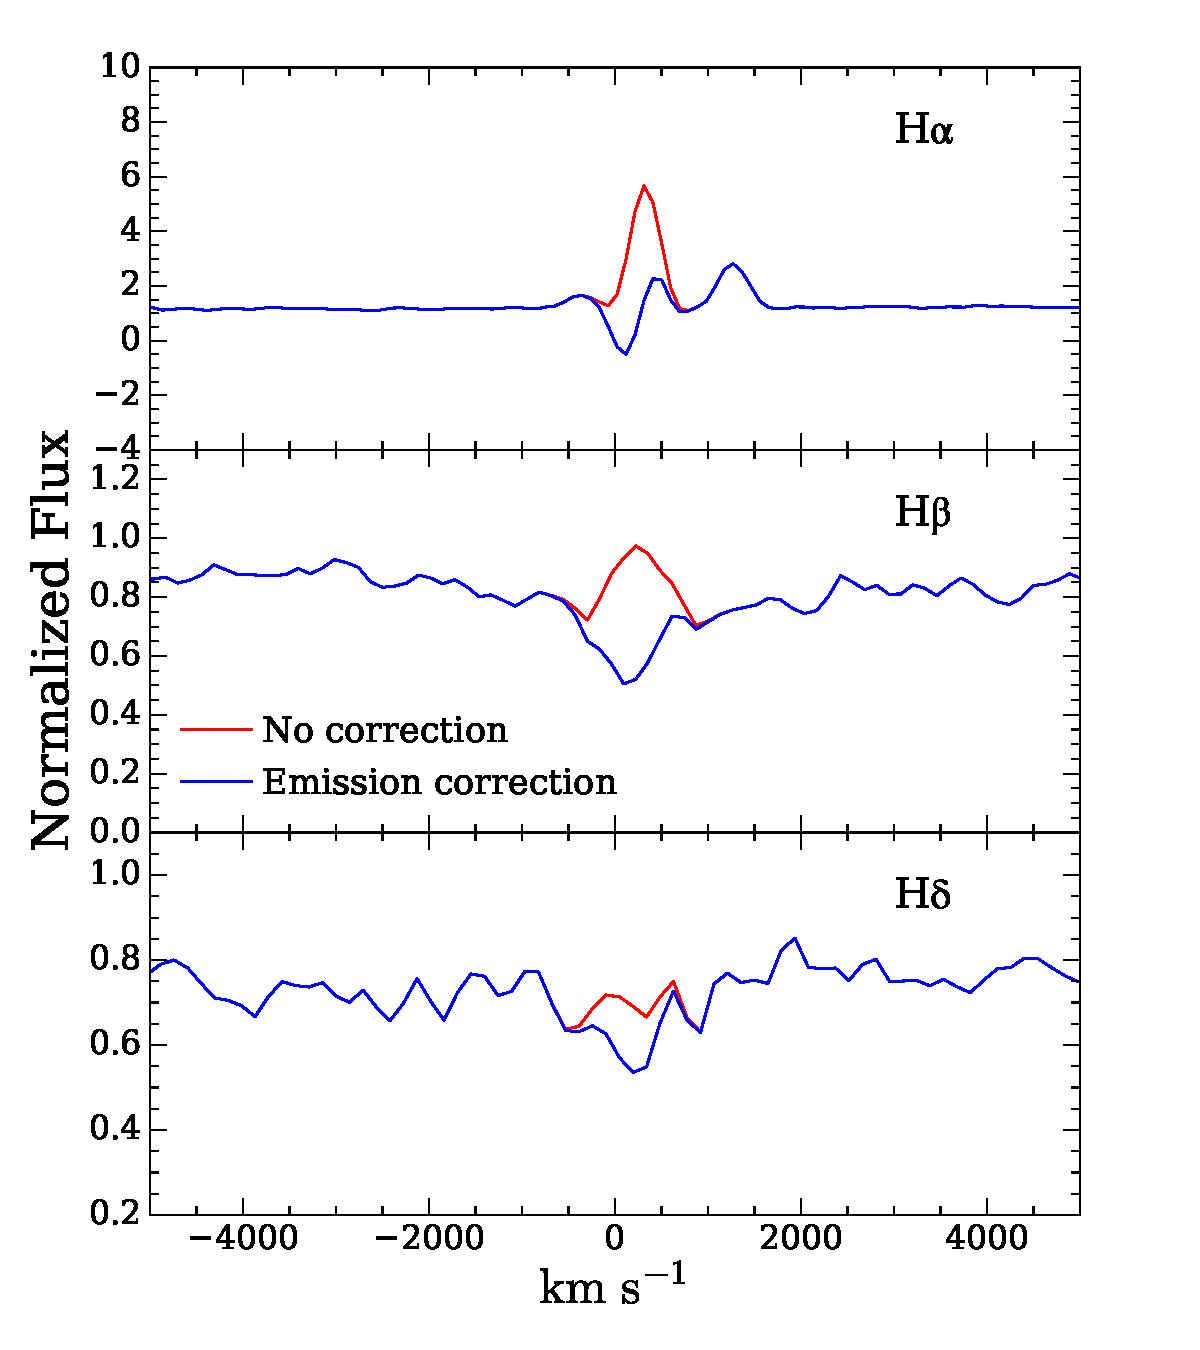
\includegraphics[width=\columnwidth]{891_2/figs/emission_comp_zoom.pdf}
  \caption[Spectra before and after Balmer emission
    correction]{\fixspacing\label{891_2:fig:emission_comp}An example
    of Balmer emission correction. The red and blue spectra show an
    aperture with strong Balmer emission (aperture P4.6) before and
    after the Balmer emission model described in
    \S\ref{891_2:sec:emission_corr} is applied.}
\end{figure}

Finally, the emission model is scaled so the \Ha flux matches the \Ha
flux measured in each individual aperture. The data spectra are then
corrected by subtracting the corresponding emission model. Figure
\ref{891_2:fig:emission_comp} shows an example of a spectrum with strong \HB
emission before and after subtracting the Balmer emission model. In
many apertures the blending of the \Ha/[NII] complex causes imperfect
subtraction in this region (as it should, our emission model does not
contain [NII] emssion), and in subsequent analysis we do not fit
(i.e., mask) data within \val{\pm 500}{\kms} of \Ha (which includes
both [NII] lines).

In addtion to \Ha/[NII] we mask other strong sources of nebular
emission ([OIII]$_{4959}$, [OIII]$_{5007}$, and S2) and sky lines with
strong residuals ([OI]$_{6300}$, NaD, and OI$_{5577}$).

%++++++++++++++++===
%% {\bf MAB: Itemize the lines that you mask -- all of them -- and give
%%   equivalent pixels to 500 \kms at the wavelength extrama. For Figure
%%   4 I can't see anything in this figure so I recommend you show
%%   blow-ups in wave for the Balmer lines from $\alpha$ to $\epsilon$.}

As mentioned above, the best-fit, extinction-value, emission-model
analysis steps are interconnected and at least one iteration is
required to find the ``final'' values.




\section{Line of Sight Depths}
\label{891_2:sec:LOS}

\begin{figure*}
  \centering
  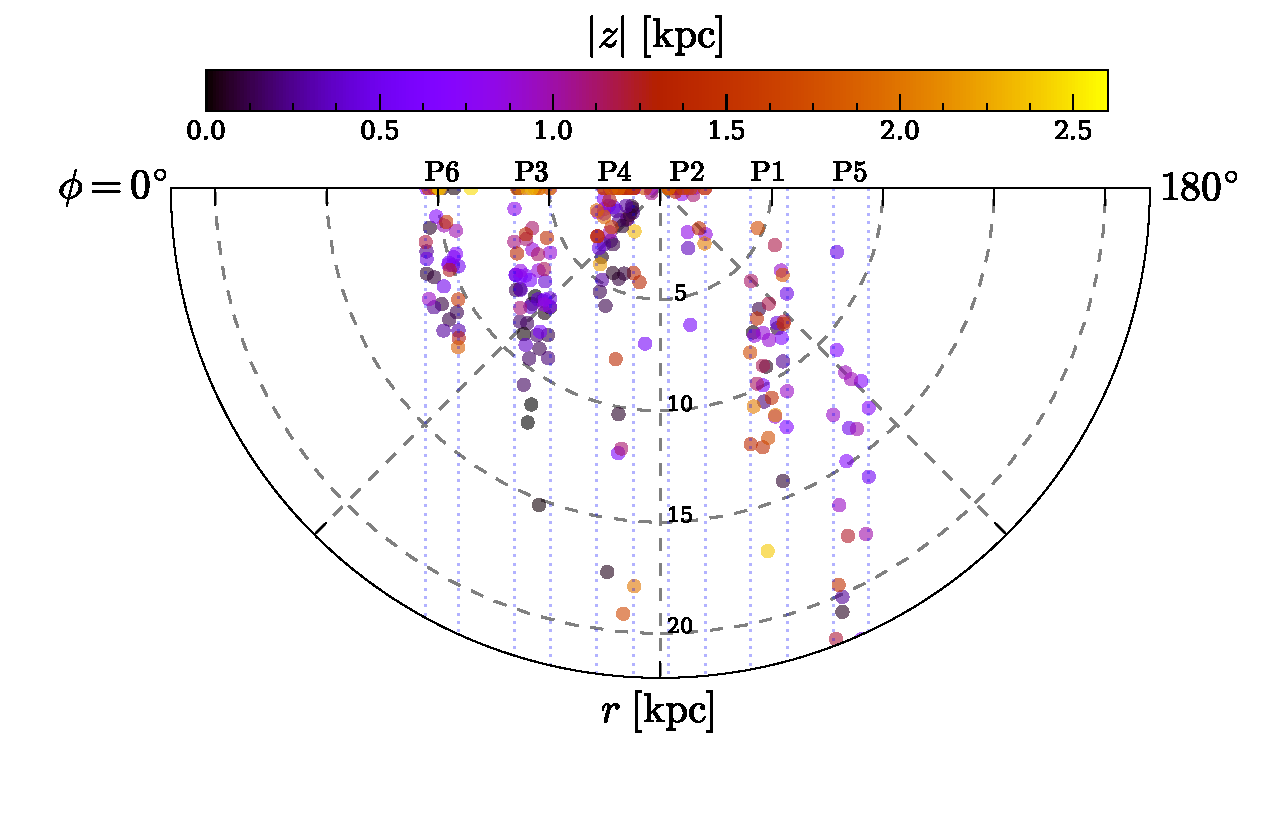
\includegraphics[width=0.9\textwidth, trim={0 1.5cm 0 0}, clip]{891_2/figs/velocity_projection.pdf}
  \caption[Map of \GP apertures in cylindrical
    coordinates]{\fixspacing\label{891_2:fig:velocity_projection}Map
    of the physical location of average emission from each aperture,
    as determined by a velocity-based LOS depth calculation (equations
    \ref{891_2:eq:vel_LOS}). The vertical dotted lines show the
    boundaries of the \GP pointings described in \ref{chap:891_1}.}
\end{figure*}

To report our quantities of interest as a function of height and true,
galactic radius we need to deproject our measured radii into radii
defined with respect to the true center of NGC 891. This deprojection
relies on understanding the average line-of-sight (LOS) depth to the
emitting material in each \GP aperture. This LOS depth can be computed
from the measured tangential velocity in each aperture.

In the absence of any attenuating material (i.e., dust) the maximum
velocity measured in each aperture will be the tangential speed of the
galaxy at any given radius and height, which, to first order, is well
approximated by the circular speed of the galaxy.  In reality,
however, when looking through an edge-on disk with high attenuation
the measured velocity is the projected velocity of emitting material
along the entire sight-line, which will become opaque before reaching
the tangent point. Thus, by comparing the measured velocity to the
known circular velocity at a given radius we can determine the LOS
depth to the emitting material.

Under the assumption that all material in the galaxy rotates at the
circular speed the relation between measured and circular velocity
comes from simple geometry. Given a measured projected radius and
velocity, $r_{\mathrm{proj}}$ and $V_{\mathrm{obs}}$, respectively,
the effective location of the emitting material in cylindrical
coordinates centered on the galaxy is
\begin{align}
  \label{891_2:eq:vel_LOS}
  \phi &= \cos^{-1}\left(\frac{V_{\mathrm{obs}}}{V_{\mathrm{c}}}\right)\\
  r &= r_{\mathrm{proj}}\frac{V_{\mathrm{c}}}{V_{\mathrm{obs}}},
\end{align}
where $V_{\mathrm{c}}$ is the circular velocity. Due to the nearly
perfect edge-on nature of NGC 891 the projected radius,
$r_\mathrm{proj}$, can be measured directly as the on-sky distance
from the galaxy center. Measurements of $V_\mathrm{obs}$ are described
in \S\ref{891_2:sec:vel}.

To compute $V_c$ we construct a simple model rotation curve using
circular velocities derived from envelop-fitting the HI data of
\citet{Swaters97}. We also include the height-dependence on circular
speed reported by \citet{Oosterloo07}. These measurements of the
circular speed are based on collisional particles (i.e., gas) and are
therefore not perfect estimates for the circular speed of the stars,
which will lag the gas slightly due to asymmetric drift. However, in
the absence of measurements of the true, stellar circular speed the
gas velocities make an acceptable approximation. Our rotation curve
for NGC 891 is thus
\begin{multline}
  V_{\mathrm{c}}(r_{\mathrm{proj}},z) =
  (\val{-15.79}{\kms})\left(\frac{z}{\mathrm{kpc}}\right) \\ 
  + \left\{
    \begin{array}{ll}
      (\val{68.2}{\kms})\left(\frac{r_{\mathrm{proj}}}{\mathrm{kpc}}\right)
      & r_{\mathrm{proj}} < \val{3.3}{kpc}\\ \val{225}{\kms} &
      r_{\mathrm{proj}} \geq \val{3.3}{kpc}.\\
    \end{array}
    \right.
\end{multline}

%+++++++++++++++++++=
%% {\bf MAB: Note sentence I broke out about HI measuing circular
%%   speed. This needs a reference and also discussion up front of how
%%   you are going to use the measured variation in this speed with
%%   height from Oosterloo07. This should be noted again in the sentence
%%   starting with the sentnece ``Under the assumption...'' You can still
%%   leave your model to the end of the par. More broadly you want to
%%   discuss whether the trends in HI tangential speed with height is
%%   representative of the potential or a lagging gas halo that may not
%%   reflect the stellar tangential speed. Similarly, you should not the
%%   amplitude of the rotation and the vertical correction relative to
%%   asymmetric drift. I think the point is that the model is not perfect
%%   for stars, but seems a reasonable approach to the best
%%   approximation. 
%------------------
%    You should discuss how uncertainties in the velocity
%%   model project to uncertainties in the inferred LOS depth, nothing
%%   that this is unlikely to introduce differential effects between the
%%   two halves of the galaxy.

%++++++++++++++++++=
%%   I am wondering about this sentence: ``In reality, however, when
%%   looking through an edge-on disk with high attenutation the measured
%%   velocity is the projected, LOS velocity of the emitting material at
%%   approximately 1 optical depth.'' Is this right and how to we
%%   reconcile it with the fact that we measure optical depths
%%   considerably greater than 1 in many lines of sight?

%++++++++++++++++=
%%   I would say something slightly different than `` we can determine
%%   the LOS depth to the emitting material.'' We are measuring a
%%   characteristic mean depth.
%++++++++++++++++
%%   Let me recommend that you simplify eqn 14. by specifying that r and
%%   z have units of kpc (you should go back and do the same for eqn. 11
%%   in the previous setion). Also note format of km s$^{-1}$.

%% }


Figure \ref{891_2:fig:velocity_projection} shows each aperture in its
velocity-derived cylindrical coordinate. We define the approaching
side of the galaxy ($r_\mathrm{proj} < 0$) to be at $\phi <
90^{\circ}$ and the receding side to have $\phi > 90^{\circ}$. With
this view the large-scale structure of NGC 891 becomes clear;
sight-lines to the receding side of NGC 891 probe the back of a spiral
arm, where \citet{Kamphuis07b} identifies a higher concentration of
dust, and as a result our measurements do not sample very far into the
disk. Conversely on the approaching side we see the leading edge of a
spiral arm, which has less dust due to ongoing star formation. On the
approaching side of the galaxy there is also a clear trend that we see
farther into the disk at larger heights, which is consistent with dust
occupying a disk with a surface density that decreases with height.

%+++++++++++++++++++
%% {\bf MAB: Explain your coordinate system in the sense of what $\phi$
%%   values correspond to approaching and receding sides. I think you can
%%   get away with the Kamphuis07 (a or b) ref here at least in terms of
%%   the spiral arm picture. What I am wondering about is if you want to
%%   address something about the phase-angle and pitch of the arms
%%   (qualitatively) in order to justify your picture here. 
%-----------
%    Also, for the
%%   last sentence concerning height, this is very difficult to see from
%%   Fig 5. Have you tried plotting $R_{proj}/R_{LOS}$ (where I think
%%   $R_{LOS}$ is your r in eqn 13) vs z, marking for approaching vs
%%   receding? Or maybe it should be $R_{LOS}/R_{proj} - 1$ vs z. }

% \subsection{Extinction-based LOS Calculations}
% We can also estimate the LOS depth based on the measured optical depth in each
% aperture. Under the massively simplifying assumption that all of the
% attenuating material in NGC 891 occupies a doubly-exponential disk we can
% calculate the extinction coefficient at any point in the galaxy:
% \begin{equation}
%   \kappa(r,\phi,z) = \kappa_{V}\rho_0\exp\left(-\frac{r}{h_r}-\frac{|z|}{h_z}\right),
% \end{equation}
% where $r$, $\phi$, and $z$ are cylindrical coordinates, $\rho_0$ is density of
% dust at $r=z=0$, and $h_r$ and $h_z$ are the dust scale length and scale
% height, respectively. The optical depth at a given projected radius,
% $r_{\mathrm{proj}}$, and LOS depth, $y$, is then
% \begin{equation}
%   \tau_V(r_{\mathrm{proj}},y,z) = \exp\left(-\frac{|z|}{h_z}\right)\rho_0\kappa_V\int_0^y \exp\left(-\frac{\sqrt{r_{\mathrm{proj}}^2 + y'^2}}{h_r}\right) d y'.
% \end{equation}
% For our analysis we use values of $h_z=\val{0.29}{kpc}$,
% $h_r=\val{7.68}{kpc}$, and $\rho_0\kappa_V = \val{1.47}{m^{-1}}$, all taken
% from \citet{xilouris99}. {\bf NOTE: CHECK THE VALUE OF $\rho_0\kappa_V$}.

% In practice we compute the $\tau_V$ integral numerically for a grid of $y$
% values and then find the value of $y$ that matches \tauV measured from SSP
% fitting (\S\ref{891_2:sec:SSP_modeling}). Figure \ref{891_2:fig:tau_projection} shows each
% aperture in its \tauV-derived cylindirical coordinate. Note that right now
% this looks pretty messed up; at the largest heights the implication is that we
% can see through the entire galaxy. Maybe this isn't so crazy at \val{2}{kpc},
% but in that case why do we still measured $\tauV > 1$?

% \begin{figure}
%   \centering
%   \includegraphics[width=\columnwidth]{891_2/figs/tau_projection.png}
%   \caption{\label{891_2:fig:tau_projection}Map of the physical location of average
%     emission from each aperture, as determined by a \tauV-based LOS depth
%     calculation. The vertical dotted lines show the boundaries of the \GP
%     pointings shown in Figure \ref{891_2:fig:pointings}. Using the simple galaxy
%     model described in the text we find that many of the apertures show
%     measured \tauV values far above what would be expected at larger
%     heights. {\bf We need to confirm we're using the correct values. Also,
%       what about clumpiness, etc.?}}
% \end{figure}


% tau_balm vs tau_cont compared to predictions from e.g. Charlot
% projected radius map from velocity vs projected radius map from A_V


\section{SSP Basis Sets}
\label{891_2:sec:SSP_sets}

Generating synthetic spectra that fit our data in a $\chi^2$ sense is
not very difficult or illuminating. A ``good'' fit is good only in the
sense that a collection of SSPs was added together with a set of
weights (Equation \ref{891_2:eq:SSP_galaxy}) that reproduce the spectrum of
our galaxy with a reasonable degree of accuracy. Degeneracies between
SSPs that have different underlying ages or metallicities but similar
spectra (and therefore can contribute equally to ``good'' fits) make
an accurate recovery of SFH, age, and metallicity difficult. To
maximize the amount of information we get from full-spectrum fits we
need to use an SSP library that a) produces ``good'' fits, and b)
minimizes internal degeneracies to increase the precision on derived
parameters (i.e., SFH, age, metallicity, and extinction).

In this section explore different methods of combining information
from SSPs with different ages and metallicities
(\S\ref{891_2:sec:bc03_SSP}). We then discuss a statistically
motivated way to reduce the number of free parameters in our fits
(\S\ref{891_2:sec:bc03_dfk}) and examine systematic differences
between different SSP libraries (\S\ref{891_2:sec:ma11}). The final
SSP library used for analysis of NGC 891 is discussed in
\S\ref{891_2:sec:final_SSP}.

Before any analysis, all model SSPs are degraded to match the spectral
resolution of our data. As discussed in Chapter \ref{chap:891_1} this
resolution is a function of both \GP fiber size and wavelength.

%++++++++++++++++++==
%% {\bf MAB: I would say this differently. First I would expound on that
%%   nature of SPS as a weighted sum of SSPs that reflect an assumed,
%%   constrained, or otherwise simulated SFH and extinction (refer back
%%   to your eqn. 1). Being able to produce a good SPS fit to the
%%   observed spectra is a necessary but not sufficient condition to
%%   achieve astrophysical insight in to the SFH, and hence and and
%%   metallicity distributions, because of the inherent degeneracies in
%%   the SPS fitting, specifically in the trade-offs between different
%%   SSP weights that have sigificant impact on inferred astrophysical
%%   properties (SFH and Z), but yield the same quality spectral fit. As
%%   a consequence, the first order of business is to determine if the
%%   necessary condition can be met (and if different SPS are a major
%%   issue for our observed data and wave range), and then to figure out
%%   how to minimize the degeneracy in a way that exploits real
%%   information in the spectra. What the latter means is not fooling
%%   ourselves about resolving SFH over age ranges where we have no
%%   diagnostic power, namely, at older ages.

%%   Then you want to give a road-map to the remainder of the
%%   section. You give a bit in 5.1, but let's put it all up
%%   front. Something like...

%%   In this section we explore the impact of fitting mono-Z vs multi-z
%%   (word this better) with the aim or criteria of X and Y. Attempts to
%%   make a more sophisticated stellar pop. age-dependent extinction
%%   model.  The above are a motivation for a down select based on
%%   something known as DFK. We also checked other SPS models to explore
%%   systematics, and then conclude on our final choice.

%% }

\subsection{Variations in Treating Metallicity and
  Extinction}
\label{891_2:sec:bc03_SSP}
The first class of SSPs used all come from \citet{Bruzual03}
(hereafter \citetalias{Bruzual03}) and use the the same 10 age bins
used by \citet{Tremonti04} (in Gyr: 0.005, 0.025, 0.1, 0.286, 0.64,
0.904, 1.434.2.5, 5, and 10).  Within these ages we also explored six
metallicities (\val{0.005}{\Zsol}, \val{0.02}{\Zsol},
\val{0.2}{\Zsol}, \val{0.4}{\Zsol}, \val{1}{\Zsol}, and
\val{2.5}{\Zsol}).

Using this basis set we tried three different mixing/fitting methods,
described below.

\subsubsection{Mono-Metallicity SSPs}
\label{891_2:sec:mono_metal}

The most basic libraries we used are 10 SSPs corresponding to the ages
listed above all at a single metallicity. To probe different
metallicities we construct a single library for each of the six
metallicities listed above and run separate fits for each one. The
final ``best'' metallicity value in each aperture is then determined
to be the mono-metallicty fit with the lowest $\chi^2_\nu$ value.
Assuming that all the separate metallicity fits represent the same
underlying photon distribution (i.e., NGC 891) and therefore sample
from the same $\chi^2$ distribution (one that contains the ``correct''
model) we can compute a confidence limit in metallicity space by
considering $\Delta\chi^2$. Here $\Delta\chi^2$ is simply the
difference in $\chi^2$ for each metallicity from the metallicity with
the lowest $\chi^2$ value. Following the example of \citet{Wall03},
the probability that a best fit with value $\chi^2 = \chi^2_i$ comes
from the same distribution (and is therefore a valid fit) as a model
with $\chi^2 = \chi^2_{\mathrm{min}}$ is\footnote{$\Delta\chi^2$ and
  Equation \ref{891_2:eq:chi_cdf} do \emph{not} correspond to reduced
  $\chi^2$. In practice all of our fits have the same number of
  degrees of freedom so this distinction is irrelevant.}
\begin{equation}
\label{891_2:eq:chi_cdf}
\alpha(\Delta\chi^2,k) = \int_0^{\Delta\chi^2}\frac{t^{(k-2)/2}e^{-t/2}}{2^{k/2}\Gamma (k/2)}dt
\end{equation}
where $\Delta\chi^2 = \chi^2_i - \chi^2_{\mathrm{min}}$, $k$ is the number of
free parameters, and $\Gamma$ is the gamma function. Equation \ref{891_2:eq:chi_cdf}
is simply the cumulative distribution function of the $\chi^2$ distribution.

Once the probabilities have been computed we reject any metallicities
with $\alpha < 0.68$. The final reported age is then the average of
$\tau_L$ over the remaining metallicities, and a good estimate of the
$\tau_L$ uncertainty caused by degeneracy in metallicity is the
corresponding standard deviation.

%% {\bf MAB: The above is very nicely described. Do we want to say
%%   anything here about whether we think the approach yields reasonable
%%   results, i.e., is a plausible statistical models? I am thinking
%%   about this sentence: ``...all the separate metallicity fits come
%%   from the same $\chi^2$ distribution (one that contains the
%%   ``correct'' model)...''  What is the ``fit''? Is it the model
%%   constructed out of N weights for the different SSP ages of a given Z
%%   plus an attenuation? Is there anything about the fits that we accept
%%   or reject that might lead us to believe the statistical criterion is
%%   reasonable?}

One drawback of this fitting method is that SSPs of all ages are
forced to have the same metallicity. Additionally, while different
apertures are allowed to have different metallicities, the metallicity
resolution is constrained to the grid of metallicities defined in
\citet{Bruzual03}.

\subsubsection{Multi-Metallicity SSPs}
\label{891_2:sec:multi_metal}
To address the metallicity issues mentioned above we next explored an
SSP library that sampled all SSP ages and metallicities
\emph{simultaneously}. In other words, each age bin of stars is
allowed to contribute flux from an arbitrary combination of SSPs at
different metallicities; instead of fitting 10 ages six times (one for
each metallicity) we now fit 60 SSPs (10 ages times 6 metallicities)
all at once. The reported metallicity is the the mean, light-weighted
metallicity described in Equation \ref{891_2:eq:MLWZ}.

\begin{figure}
  \centering
  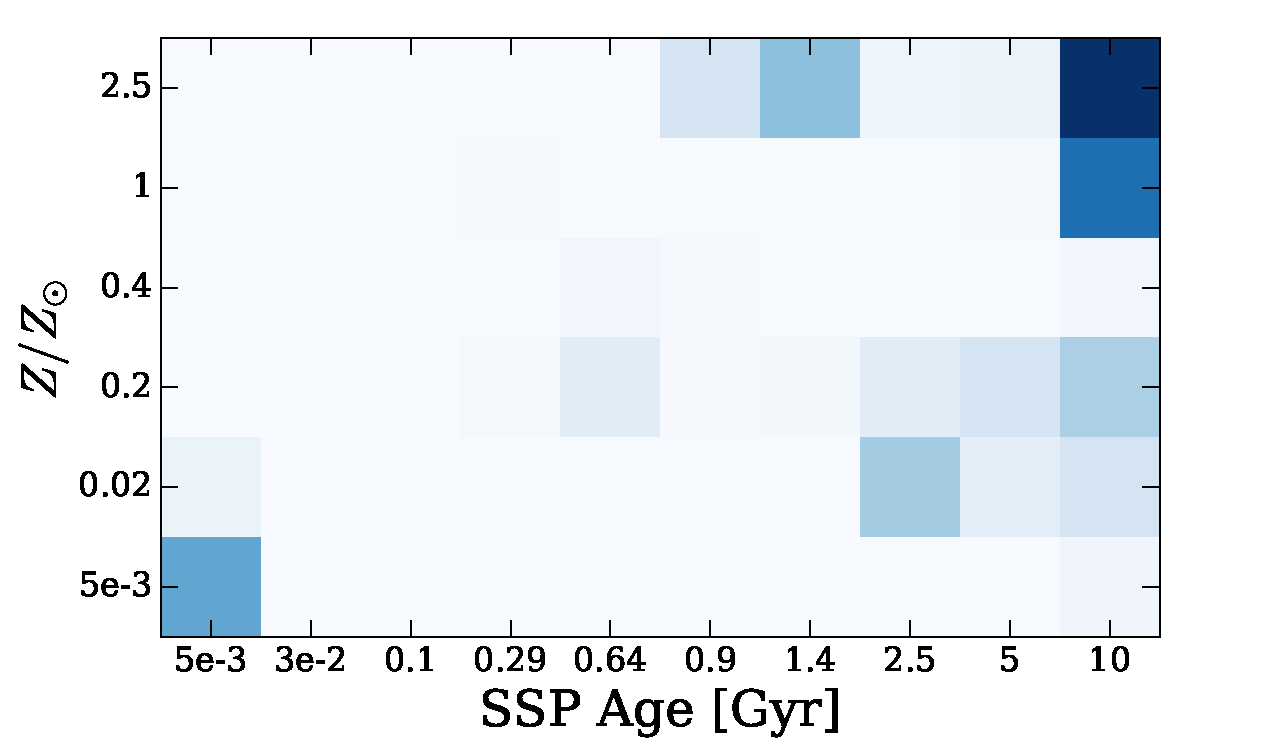
\includegraphics[width=\columnwidth]{891_2/figs/allZ2_all_weights.pdf}
  \caption[Example of SSP light-weights for 61 parameter
    fit]{\fixspacing\label{891_2:fig:multiZ_weights}SSP light weights
    across all apertures in all pointings for the multi-metallicity
    SSP basis set. Each square shows the light weight, $W_{L,i,j}$,
    for SSP age $t_i$ and metallicity $Z_j$, averaged across all 261
    apertures. Before averaging each aperture is normalized to the
    same total flux so that the darkness of the box represents a true
    comparison of the relative contributions of each SSP across the
    all apertures.}
\end{figure}

Unlike the mono-metallicity libraries our multi-metallicity SSP
library allows for a more physically realistic picture NGC 891, one in
which each location in the galaxy is a superposition stellar
populations with different formation ages and metallicities. This
additional information comes at a cost, however; 60 free parameters
(plus one for the extinction) can lead to degeneracies that severely
dilute our ability to precisely interpret the results of our fits.

\begin{figure}
  \centering
  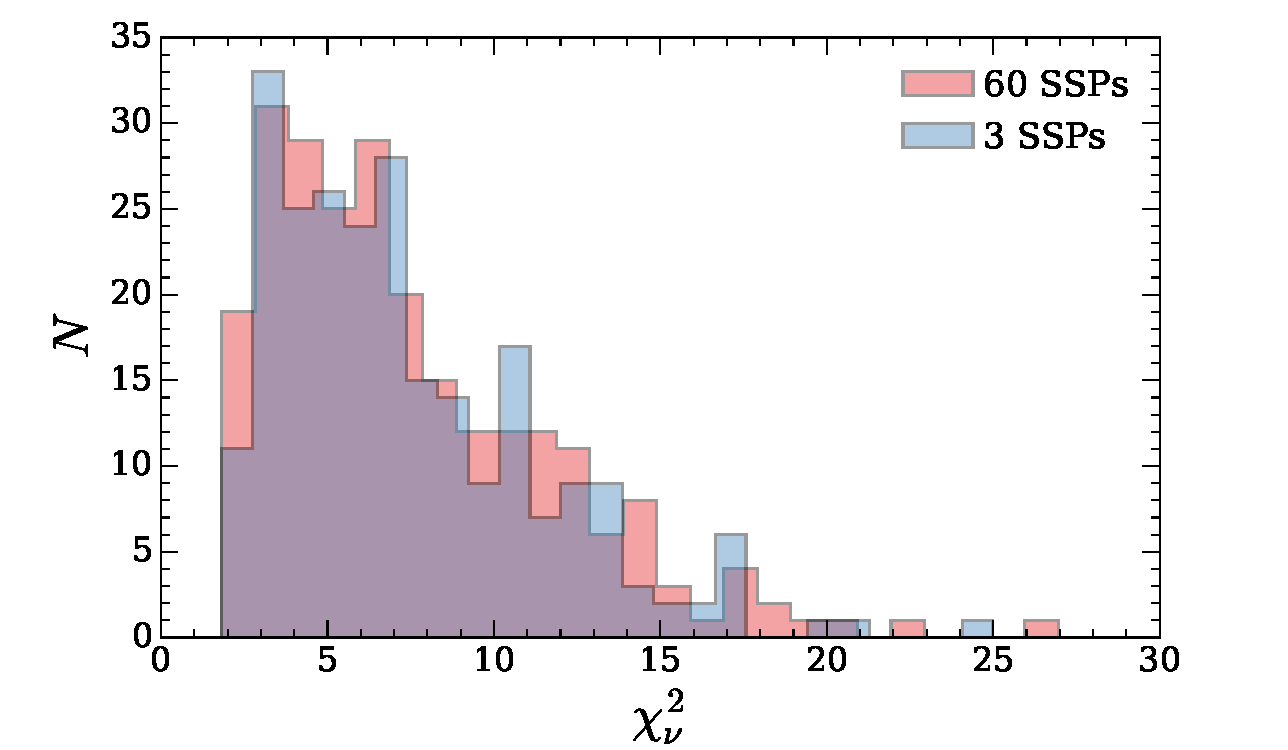
\includegraphics[width=\columnwidth]{891_2/figs/allz_chihist.pdf}
  \caption[$\chi_{\nu}^2$ distributions for template libraries with 60
    and 3 SSPs]{\fixspacing\label{891_2:fig:3SSP_chi}Distribution of
    best-fit $\chi^2_\nu$ values for the full, multi-metallicity basis
    set described in \S\ref{891_2:sec:multi_metal} (\emph{red}) and a
    artificially down-selected basis set containing only 5, 904, and
    \val{1000}{Myr} SSPs 1 \Zsol (\emph{blue}). A 2-sample KS test
    indicates these two distributions come from the same underlying
    distribution with $p > 0.99$.}
\end{figure}

Figure \ref{891_2:fig:multiZ_weights} shows an example of the
age/metallicity parameter space spanned by this method. We find that
60 SSPs generally over-constrain the spectral fitting and only \asim 5
SSPs contribute significant flux. To further investigate these
degeneracies we constructed a test basis set that contained only 3 of
the 60 SSPs described above: 5, 904, and \val{1000}{Myr} SSPs all at
solar metallicity. We then compared the distributions of best-fit,
reduced $\chi^2$ values resulting from fitting 60 SSPs to fits using
only 3 SSPs. As shown in Figure \ref{891_2:fig:3SSP_chi} these two
$\chi^2_\nu$ distributions look remarkably similar and a 2-sample KS
test confirms that they are drawn from the same distribution with $p >
0.99$. 

This result confirms the claim that 60 SSPs over-constrain our fits,
but doesn't' provide a satisfying resolution; the choice of the three
SSPs used in the comparison was largely arbitrary and similar results
can be obtained regardless of the specific SSPs used. In other words,
we lack the ability to downselect from 60 SSPs in a physically or
statistically motivated way. In \S\ref{891_2:sec:bc03_dfk} we argue
that a downselection based on diffusion k-means can solve this
problem.

%% {\bf MAB: yet again, well described and a compelling example. I
%%   suspect this general result has some precedent in the
%%   literature. Have you checked?}

%% ADE comment: no

\subsubsection{Multi-Extinction SSPs}

In the above cases we apply a single extinction parameter to all SSPs
within an aperture, however models of dust in galaxies often prescribe
separate extinctions for different age populations. In a basic example
\citep{Charlot00} stars younger than \val{30}{Myr} are still shrouded
in an HI envelope and therefore experience more attenuation of their
light. We can simulate this type of behavior by allowing each SSP to
have its own value of \tauV so that Equation \ref{891_2:eq:SSP_galaxy}
becomes
\begin{equation}
g(\lambda,Z) = \sum_{i} R(\lambda,\tau_{V,i}) M(\Delta t_i,Z)
f(\lambda,\Delta t_i, Z).
\end{equation}
This raises the number of fit parameters from 11 (10 $M(\Delta t_i, Z)$
values and 1 \tauV) to 20 (10 $M(\Delta t_i, Z)$ and 10
$\tau_{\mathrm{V,cont},i}$).

In practice this library produced fits that failed to converge on
reasonable timescales (days) and was abandoned. We note, however, that
the reduction in parameters provided by the method discussed in the
next section might make this problem tractable. Future work in will
investigate the resurrection of a multi-extinction SSP mix.

\subsection{Diffusion K-Means BC03 SSPs}
\label{891_2:sec:bc03_dfk}

An attractive way to address the issues arising from a large SSP
library (e.g., degeneracies and hence lack of precision in fit
parameters) is to simply reduce the total number of SSPs used
\citep[e.g.,][]{Tremonti04, CidFernandes05, Tojeiro07}.
%% One of the biggest issues with the a large set of SSPs is that they create a
%% flat $\chi^2$ space and lead to degenerate solutions (as shown if
%% Figs. \ref{891_2:fig:multiZ_weights} and \ref{891_2:fig:bc03_chisq}). To put it another
%% way, I have found ({\bf and will show}) that full spectrum fits of the same
%% quality (i.e., $\chi^2$) as the full BC03 library can be produced with a very
%% small SSP library (even as small as 2-3 SSPs). Of course, in this case a good
%% $\chi^2$ value means almost nothing because there will be no physical
%% reasoning or understanding behind the SSPs used.
The diffusion k-means (DFK) method of \citet{Mosby15} (hereafter
\citetalias{Mosby15}) directly achieves this reduction of parameter
space in a statistically and physically motivated
way. \citetalias{Mosby15} take all 107 solar metallicity
\citetalias{Bruzual03} SSP templates and place them in a
three-dimensional diffusion space (a reduction from the $> 1000$
wavelength channels) through a process called \emph{diffusion
  mapping}. During this mapping \citetalias{Mosby15} only consider
wavelengths in the range
$\val{3600}{\AA}\leq\lambda\leq\val{8500}{\AA}$, which fully covers
the wavelength range of our \GP data. The templates are then grouped
into bins based on how close they lie in this diffusion space, which
essentially groups the templates based on similarities in their
spectra shape. The result is 4 broad age bins that capture important
differences between different aged populations. The age range of these
bins is shown in Table \ref{891_2:tab:dfk} and we refer to them as Young
(Y), Intermediate 1 (I1), Intermediate 2 (I2), and Old (O).

\begin{deluxetable}{ccr}
\tablewidth{0pt}
\tablecaption{Diffusion k-means bins}
\tablehead{ 
  \colhead{DFK group} &
  \colhead{M15\tablenotemark{a} label} &
  \colhead{Age range}
}
\startdata 
1 & Y & 0.9-5.2 Myr \\
2 & I1 & 5.5-404 Myr \\
3 & I2 & 453.5-5750 Myr \\
4 & O & 6000-13500 Myr
\enddata
\label{891_2:tab:dfk}
\tablenotetext{a}{\citet{Mosby15}}
\end{deluxetable}

It is important to note that \citetalias{Mosby15} find that simply
using the median \citetalias{Bruzual03} SSP from within a DFK bin does
not produce a basis set that is is more precise than the full set of
\citetalias{Bruzual03} templates. The spectrum associated with each
DFK bin must be an average of all the spectra within that bin and thus
the DFK basis set constitutes a set of spectra that are different than
the standard \citetalias{Bruzual03} templates. These averages are
weighted by the time interval straddled by each of the input
\citetalias{Bruzual03} spectra and the weights used in
\citetalias{Mosby15} and in this work assume a constant star formation
across each DFK bin.

Figure \ref{891_2:fig:bc_dfk_comp} shows a comparison between the SSP
templates used in \S\ref{891_2:sec:bc03_SSP} (taken from \citet{Tremonti04})
and the reduced, DFK templates. It also highlights the evolutionary
scatter in each DFK bin: the O bin is old enough that there is almost
no change in spectral shape across the entire age range. The I1 and I2
bins, on the other hand, cover a wide range in spectral shape but are
still represented well by their single, averaged DFK spectra.

%+++++++++++++++++++
%% {\bf MAB: The REFS you want in the first sentence here will address
%%   the ones I wanted you to consider in the lst paragraph of 5.1.2.

%%   Note BC03 needs to be replaced with a ``ref'' or something.  

%%   A few things need clarification / better explainataion:

%%   I would like you to explain what the 3D diffusion space is. It's got
%%   to be related to something like the sum of the differences (squared
%%   or abs. val) of the normalized spectra.

%%   I want to know what set of SSP ages you (or Mosbt15) are using,
%%   i.e., the ones you mention in the beginning of 5.1 or a finer grid?
%%   Does it matter?

%%   The reason why the median SSP within a DFK bin does not yield the
%%   full advantage, and what this full advantage is defined to be.

%%   ``thus the DFK basis set constitues a completey different set of
%%   spectra than the standard \citetalias{Bruzual03} libraries.'' How can this be true
%%   since the DFKs are sums of BC03 SSPs? And you should clarify that
%%   when you say ``BC03 libraries'' you refer to SSP libraries; I would
%%   call these templates since libraries is a term usually reserved for
%%   the individual stellar spectra that get weighted by the evolutionary
%%   tracks to form an SSP.

%%   Clarify that the weights are actually a combination of the time
%%   interval of the SSP and assumed SFH. Does the advantage of the DFK
%%   depend on the assumed SFH?

%%   In the last sentence clarify if ``in this work'' refers to Mosby15
%%   or this paper.

%%   Over what wavelength has the DFK analysis been done? (this is
%%   important for below).

%% }

%% , but we assign ages to each SSP by computing a
%% mass weighted age from the SSPs in each bin. Assuming a constant start
%% formation history (as do \citet{Mosby15}) the weight of each SSP is
%% \begin{equation}
%%   \label{891_2:eq:dfk_weight}
%%   w_i = \left\{
%%     \begin{array}{ll}
%%       \frac{t_1+t_2}{2} & i =1\\
%%       \frac{t_{i+1}-t_{i-1}}{2} & i\neq1~\mathrm{and}~i\neq N\\
%%       \frac{t_N - t_{N-1}}{2} & i = N,
%%     \end{array}
%%     \right.
%% \end{equation}
%% where $t_i$ are the ages of the individual SSPs and $N$ is the total number of
%% SSPs (107). Table \ref{891_2:tab:dfk} shows the age groupings and weighted ages of
%% our 4 diffusion k-means basis SSPs.

\begin{figure}
  \centering
  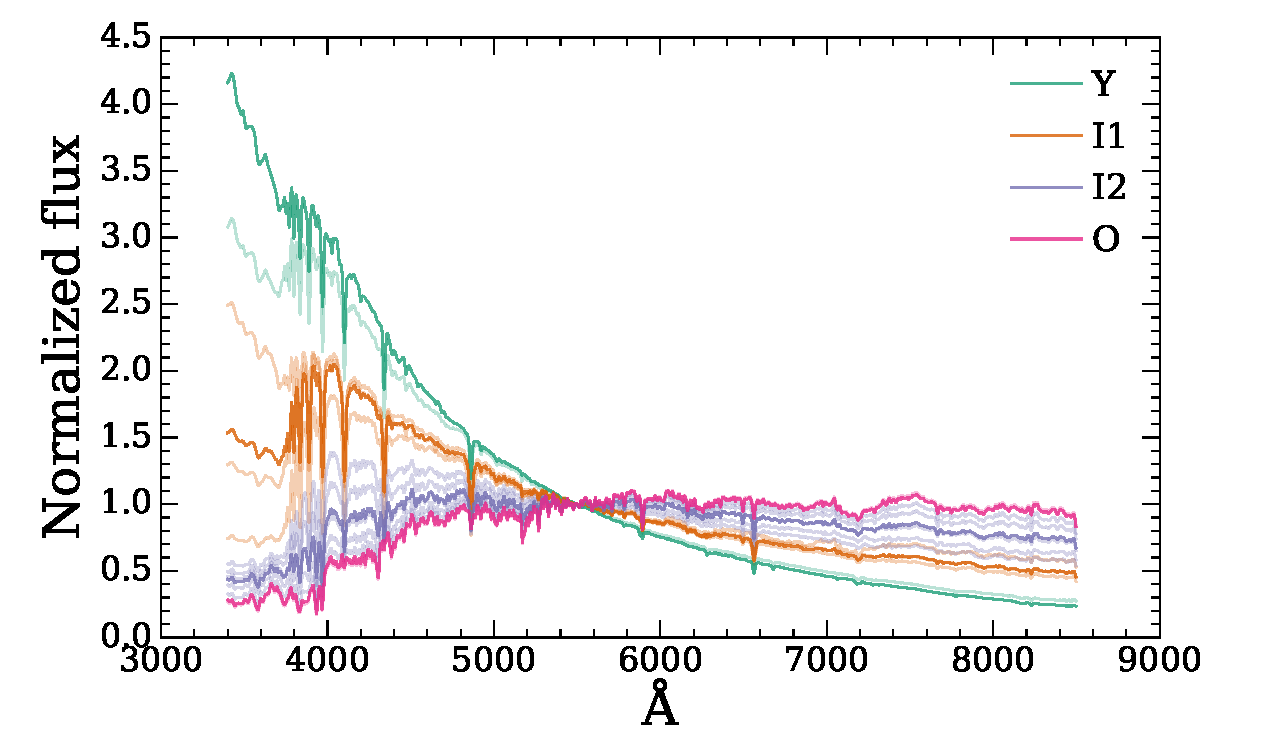
\includegraphics[width=\columnwidth]{891_2/figs/bc_dfk_comp.pdf}
  \caption[Comparison of full BC03 and diffusion k-means
    spectra]{\fixspacing\label{891_2:fig:bc_dfk_comp}The set of
    \citetalias{Bruzual03} SSPs used in \S\ref{891_2:sec:bc03_SSP}
    (lightly shaded) and the reduced basis set that results from
    applying diffusion k-means (solid). The colors correspond to the
    final groupings in diffusion K-means space (defined in Table
    \ref{891_2:tab:dfk}). Figure adapted from \citetalias{Mosby15}.}
\end{figure}

Despite being based on purely statistical methods (i.e., diffusion
k-means), the age groupings of the final bins roughly correspond to
important timescales in stellar evolution. The Young bin corresponds
to the very brightest O and B stars that have strong UV flux and
prominent Balmer absorption. Intermediate 1 covers B, A, and F stars
that have the strongest Balmer absorption. Intermediate 2 covers
timescales where the main sequence turn-off transitions from A stars
to late F stars and the total flux has major contributions from giant
branch and thermally pulsating asymptotic giant branch stars. Finally,
the Old bin contains F and G stars with strong metal lines and very
little spectral evolution over the bin. It is important to note that
\citetalias{Mosby15} do artificially adjust the limits of the oldest
two bins to account for the fact that star formation histories are
rarely constant over \val{10}{Gyr}.

%+++++++++++++++=
%% {\bf MAB: Check your MS evolutionary time-scales. I think Y includes
%%   O/B, while I1 includes B/A/F. For the I2 bin a lot happens. This is
%%   the time scale over which TP-AGB stars have significant
%%   contriutions, the bolometric flux becomes dominated by the giant
%%   branch (beyhond 1-2 Gyr), and the MS turn-off evolves from A into
%%   late F. In the oldest bin, everthing is boring; the turn-off has
%%   ground down to somewhere between late F and early G, while the red
%%   light is dominated by red giants. Might think about where HB becomes
%%   important which will be even more sensitive to metallicity than the
%%   RGB. Blue HB can compete with MS turn-off in the blue/NUV.

%%   I don't understand the statement in the last sentence for why the
%%   limits in the two oldest bins were adjusted. I actually think this
%%   is likely a mistake since 0.4-2 Gyr is likely the key phase in which
%%   TP-AGB stars play a role.

%%   On this point I asked about the wave range for establishing DFK
%%   because if it did not go very red and used BC03 it may not have been
%%   sensitive to TP-AGB. So among the limitations of the DFK that can be
%%   improved upon in the future is the treatment of metallicity
%%   variations, extention to longer wavelengths, and application to
%%   other SPS models (especially MA11) that are sensitive to variations
%%   in intermediate age populations.

%% }

One of the current limitations of this method is that the diffusion k-means
grouping has so far only been performed on solar metallicity SSPs. To
constrain metallicity we construct composite metallicity libraries in the
style of both \S\ref{891_2:sec:mono_metal} and \S\ref{891_2:sec:multi_metal} using the
exact same SSP groupings described in Table \ref{891_2:tab:dfk}. The resulting
analysis is the same as for those sections. In this sense the DFK grouping
only reduces the size of the age dimension of SSP parameter space; we still
need to deal with uncertainties in the choice of metallicity and degeneracies
between age and metallicity.

\subsection{Alternative SSP templates}
\label{891_2:sec:ma11}

The SSPs of \citet{Maraston11} (hereafter \citetalias{Maraston11})
offer an appealing, modern alternative to the \citetalias{Bruzual03}
SSPs. Namely, they avoid the known issues with Balmer absorption in
the Stelib library \citep{Groves11} by using the MILES stellar
libraries \citep{Vazdekis10,Falcon-Barroso11}. \citetalias{Maraston11}
also use the fuel consumption theorem
\citep{Renzini81,Buzzoni89,Maraston05} to address problems that arise
from using isochrones (as do \citetalias{Bruzual03}) to simulate the
rapid changes in phase that occur at the tip of the RGB, the AGB, and
the RGB bump.

\begin{figure}
  \centering
  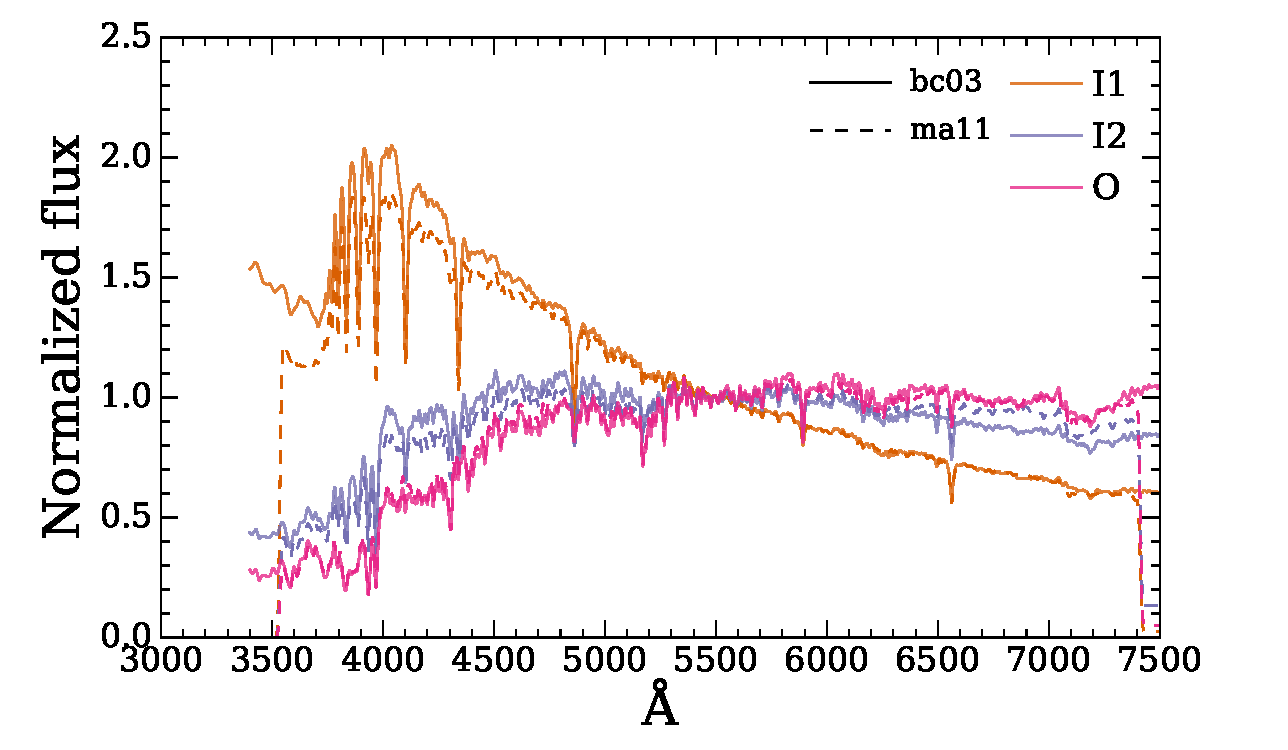
\includegraphics[width=\columnwidth]{891_2/figs/ma_bc_comp.pdf}
  \caption[Comparison of DFK BC03 and MA11 SSP template
    libraries]{\fixspacing\label{891_2:fig:ma_bc_comp}Comparison of
    diffusion k-means \citetalias{Bruzual03} and
    \citetalias{Maraston11} models. Colors correspond to DFK age bins,
    as defined in Table \ref{891_2:tab:dfk}. The solid and dashed
    lines are the \citetalias{Bruzual03} and \citetalias{Maraston11}
    basis sets, respectively. Note that the \citetalias{Maraston11}
    basis set lacks the youngest age bin and does not extend redward
    of \val{\asim 7500}{\AA}}
\end{figure}

To make as fair a comparison as possible the \citetalias{Maraston11}
models were first grouped into the same diffusion k-means bins as the
BC03 models (the consequences of using a DFK grouping from a different
set of models will be ignored for the time being). This decision comes
with one major caveat; the \citetalias{Maraston11} models do not
extend to the youngest ages sampled by \citetalias{Bruzual03}. The
youngest \citetalias{Maraston11} age is \val{6.5}{Myr}, which is
\emph{older} than the youngest bin found by \citetalias{Mosby15}. For
this reason our \citetalias{Maraston11} basis set does not have a
``Young'' SSP and thus consists of only 3 SSPs for each metallicity.


Figure \ref{891_2:fig:ma_bc_comp} shows a comparison between the
\citetalias{Maraston11} and \citetalias{Bruzual03} SSP basis sets at
\val{1}{\Zsol}. The differences in the shapes of these two basis sets
have important implications for the interpretation of the SSP fitting
results. In particular, the difference between the two models in the
blue end decreases with SSP age; the I2 \citetalias{Maraston11} SSP
has less flux than the I2 \citetalias{Bruzual03} SSP by a larger
difference than the I1 SSPs. At the oldest SSP age the
\citetalias{Maraston11} model actually produces slightly more flux
than the \citetalias{Bruzual03} model. Because of this trend the
\citetalias{Maraston11} require more mass at younger ages to match the
same spectrum as the \citetalias{Bruzual03} basis. Thus we expect the
derived $\tau_L$ values for the \citetalias{Maraston11} basis set to
be lower than those derived using \citetalias{Bruzual03} SSPs.

%+++++++++++
%% {\bf MAB: How much of the above should we say is highly dependent on
%%   the fact that we have not really done a full-up DFK on the
%%   \citetalias{Maraston11} models but are imposing the age-bins defined
%%   by M15's analysis of BC03? I.e., the differences we are finding here
%%   may not be as important or significant.}

In addition to the lack of young ages, the age resolution of
\citetalias{Maraston11} is much less than
\citetalias{Bruzual03}. Compared to \citetalias{Bruzual03}'s 107 age
bins the \citetalias{Maraston11} have at most 50 age bins (for solar
metallicity) and sometimes as few as 14. To asses whether this limited
age sampling affects the diffusion k-means averages we rebinned the
\citetalias{Bruzual03} diffusion k-means spectra from a sample of
\citetalias{Bruzual03} spectra down-selected to match the age bins of
the \citetalias{Maraston11} models. Figure \ref{891_2:fig:bc03_downselect}
shows a comparison of the \citetalias{Maraston11} and
\citetalias{Bruzual03} DFK models; down-selecting the
\citetalias{Bruzual03} models does not appreciably affect the final,
averaged DFK spectra.

Ultimately, we choose not to use the DFK'd \citetalias{Maraston11}
models, but this is primarily due to the fact that our DFK bins are
constructed specifically for the \citetalias{Bruzual03} data set. The
omission of \citetalias{Maraston11} models from subsequent analysis is
not a statement about the quality of the models themselves. We
strongly warn the reader away from making a robust comparison between
the models of \citetalias{Bruzual03} and \citetalias{Maraston11} based
on our analysis precisely for the reason that our DFK binning was
tailored for the \citetalias{Bruzual03} models.  Future work in the
area of diffusion k-means should be able to easily produce a separate
set of DFK basis spectra for the full \citetalias{Maraston11} model
set.

%++++++++++++++++++
%% {\bf MAB: I would rewrite the ``omission'' sentence. I think there are
%%   three concerns we have had with the Maraston models (1) the
%%   time-steps were coarser; (2) the time steps didn't go as young ages;
%%   (3) th DFK analysis was not done with these models. We've eliminated
%%   (1) as an issues, but as we will find in Fig 21, the youngest DFK
%%   does seem important at low heights. Given that the DFK analysis was
%%   done with the BC03 data and has this younger age bin it is prudent
%%   to continue with the BC03 spectra. However, future analysis needs to
%%   consider the \citetalias{Maraston11} models, particularly for
%%   intermediate ages when extending farther to the read where TP-AGB
%%   stars are more important.}

\begin{figure}
  \centering
  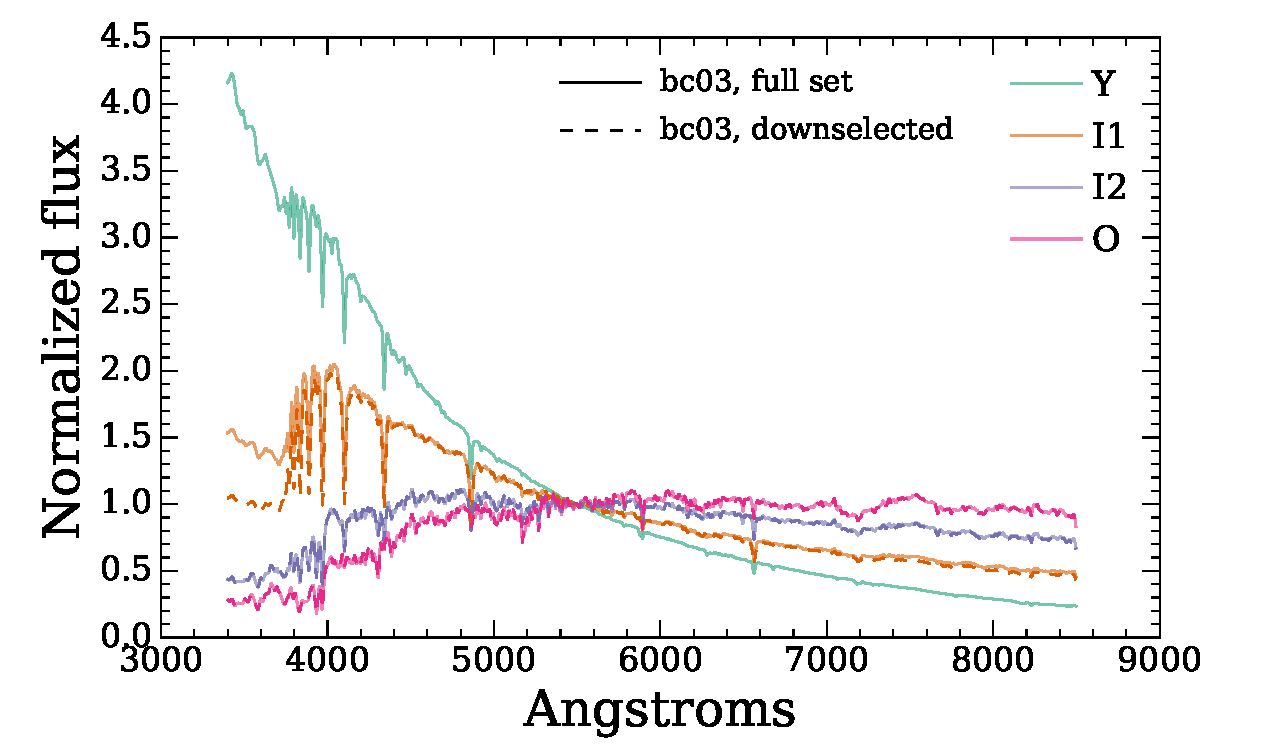
\includegraphics[width=\columnwidth]{891_2/figs/bc_downselect.pdf}
  \caption[Effect of downselecting BC03 age
    resolution]{\fixspacing\label{891_2:fig:bc03_downselect}The effect
    of downselecting the \citetalias{Bruzual03} ages to match the age
    grid of the \citetalias{Maraston11} models. This down-selection
    reduced the number of input SSPs from 107 to 50. Note that the
    \citetalias{Maraston11} age grid does not contain the youngest age
    bin.}
\end{figure}

\subsection{The final choice of SSP basis set}
\label{891_2:sec:final_SSP}
\begin{figure}
  \centering
  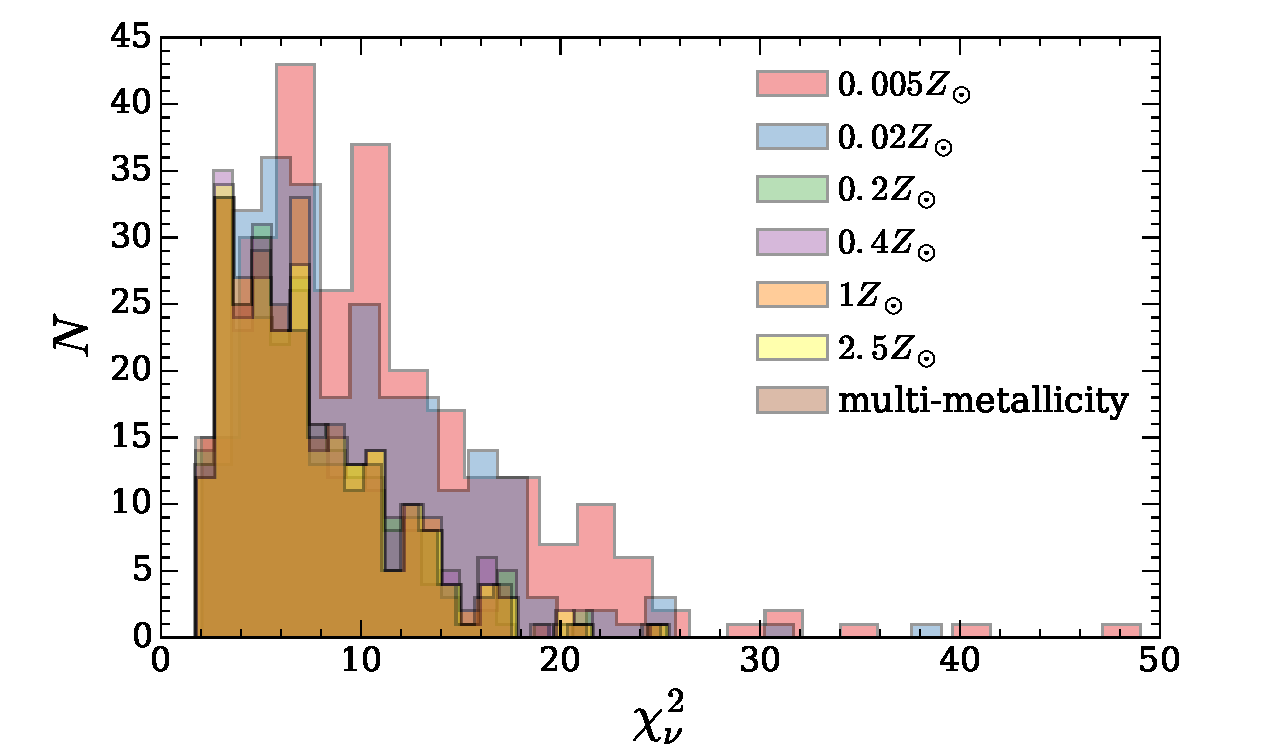
\includegraphics[width=\columnwidth]{891_2/figs/dfk_chihist.pdf}
  \caption[$\chi_{\nu}^2$ distributions for different metallicity
    fits]{\fixspacing\label{891_2:fig:chisq_hist}Histograms of
    best-fitting $\chi^2_\nu$ values for all 261 apertures using both
    mono-metallicity and multi-metallicity DFK SSP library sets.}
\end{figure}

We choose the \citetalias{Bruzual03} DFK template set as our primary
SSP library because it is statistically motivated, reduces the number
of fit free parameters (which also reduces computation time), and
approximates important epochs in stellar evolution. We do note,
however, that the DFK bins presented in \citetalias{Mosby15} are
designed for very low signal to noise data and therefore may reduce
the number of SSP templates beyond what is strictly necessary for our
data. In particular the I2 DFK bin covers a very wide range in stellar
evolution and future work might show that it can be split into
multiple bins.

%++++++++++++++
%% {\bf MAB: with a nod to the lack of an intermediate age bin, i.e.,
%%   room for future improvement. I think this or somewhere we need to
%%   recount that M15 analysis was based on VERY low S/N, so we have to
%%   explain why we think this coarse age grid is reaonably using
%%   available information with our data. (This is a major point,
%%   actually.)}

We modify the solar metallicity basis set defined by
\citetalias{Mosby15} to consider multiple metallicities using the same
method described in \S\ref{891_2:sec:multi_metal}; each age bin is
allowed to contribute light from an arbitrary number of SSPs with
different metallicities. Thus the full set contains 24 separate SSPs:
six metallicities each in the four age bins described by
\citetalias{Mosby15}. We find, however, that SSPs with metallicity
below \val{0.2}{\Zsol} are both statistically unrepresentative of our
galaxy spectra and astrophysically implausible given the expected
rapid chemical enrichment time-scales that result in a minimal
contribution from super metal-poor populations to the integrated
light.

To test this assertion we construct mono-metallicity DFK basis sets in
the same metallicity bins listed in \S\ref{891_2:sec:mono_metal} and fit
them to our data. We then compare the distributions of goodness-of-fit
(i.e., $\chi^2_\nu$) between the different metallicities and can
identify fits that are statistically different from the best fitting
model and therefore not likely representative of the true galaxy
spectrum.

Figure \ref{891_2:fig:chisq_hist} shows the $\chi^2_\nu$ distributions for
all \GP apertures for the mono-metallicity DFK basis sets and our
final choice of SSP basis set (``multi-metallicity''). The two lowest
mono-metallicity SSP sets (0.005 and \val{0.02}{\Zsol}) produce
spectral fits that occupy a different locus in $\chi^2_\nu$ and are
worse than all other metallicities. A 2-sample KS test confirms that
these two metallicities are not part of the same distribution as the
other mono-metallicity basis sets with $p \ll 0.001$. Conversely, all
other mono-metallicity basis sets are drawn from the same underlying
distribution with $p > 0.8$, in the worst case, and it is therefore
difficult to justify, in a statistical sense, choosing a single
metallicity over another. 

Figure \ref{891_2:fig:chisq_hist} also shows that our final,
multi-metallicity basis set (with only $Z \geq \val{0.2}{\Zsol}$)
produces fits of comparable quality to the mono-metallicity fits ($p >
0.8$). Thus we cannot say that our multi-metallicity basis set
provides a statistical improvement over any one mono-metallicity basis
set. The advantage, however, of the final basis set is in the physical
insight gained by creating a more realistic physical model of the
galaxy. Using a multi-metallicity SSP set also allows us to check if
astrophysically reasonable age-metallicity relations come out of our
analysis \emph{without} having to assume age/metallicity priors (as is
done in mono-metallicity basis sets). In other words, both mono and
multi-metallicity basis sets will be subject to degeneracies between
age and metallicity, but we can only quantify these degeneracies
(\S\ref{891_2:sec:fit_err}) with a multi-metallicity basis set.

%+++++++++++++++++++
%% {\bf MAB: Let me make sure I understand the histogram and
%%   comparison. For each mono-z case you are plotting the $\chi^2_\nu$
%%   distribution for fits with that metallicity to every aperture
%%   (individually). That means the $\chi^2_\nu$ distribution is
%%   statistically the same as the multi-Z case, where the mean Z is
%%   tailored for each galaxy. At first blush, that ain't good. It would
%%   suggest we have jack for leverage on Z. One related aside: How does
%%   the multi-z histogram compare to one where for every aperture you
%%   take the lowest mono-z $\chi^2_\nu$ value across all Z?

%%   Here is what I think we need to say. First, the reason why we think
%%   the $\chi^2_\nu$ distributions are so similar is because of the
%%   well-known age-Z degeneracy. Hence our exploration here is to
%%   eliminate as much Z and age that we think is either implausible
%%   (low-Z) or for which we have inadequate information to resolve (DFK
%%   age bins). With that in hand we want to use the multi-Z models to
%%   determine if astrophysically plausible age-metallicity relations
%%   come out of the analysis w/o further priors; we couldn't explore
%%   this with the mono-z models. Second, one of the reasons why we
%%   looked at altering $\chi^2$ was specifically to determine if we could
%%   improve the age-Z discrimination. This motivates the next section.

%---------------------
%%   Also, I think we talked about two side-by-side historgrams: One
%%   showing all mono-Z for $Z>0.02$ and multi-Z averaged together vs the
%%   two low-Z cases; and then on blowing up in $\chi^2_\nu$ comparing
%%   the mono-z with multi-z. I still think that is a good idea.

%% }
\begin{figure}
  \centering
  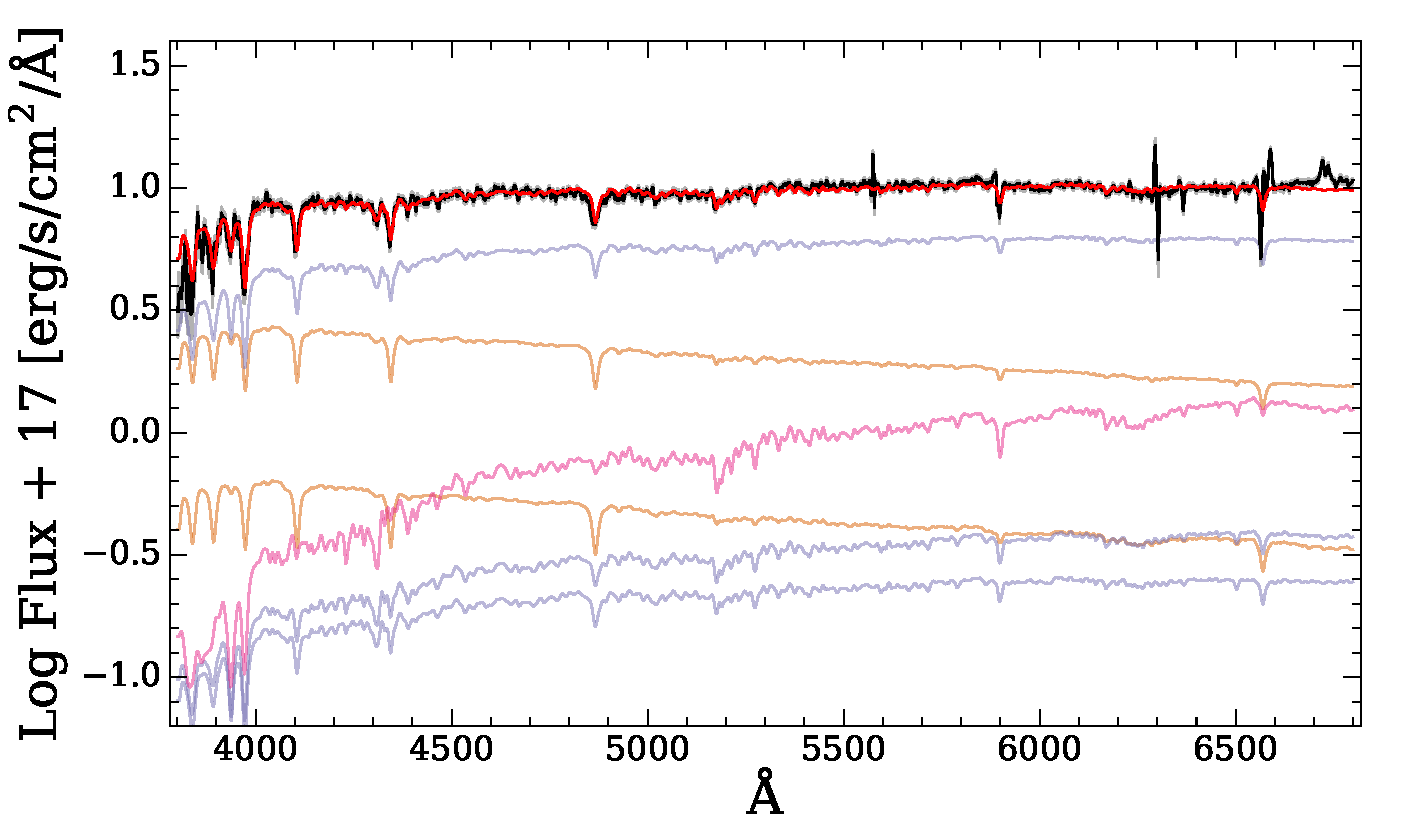
\includegraphics[width=\columnwidth]{891_2/figs/example_fit.pdf}
  \caption[Example model galaxy
    fit]{\fixspacing\label{891_2:fig:ex_fit}Example SSP fit to a
    single galaxy aperture (P6.9). The black line with gray shading
    (hard to see) show the measured flux and corresponding
    uncertainty. Each colored line (besides red) is an SSP from the
    \citetalias{Bruzual03} DFK basis set described above and the
    colors are the same as in Figure \ref{891_2:fig:bc_dfk_comp}. The
    red line is the superposition of all the individual SSP spectra.}
\end{figure}

Finally, Figure \ref{891_2:fig:ex_fit} shows an example of the best
fit in one of our apertures (pointing 6, aperture 9). This example is
typical for most apertures in our data set; the data has relatively
high signal/noise and is well fit by the superposition of our final
SSP basis set.

%-----------------
%% {\bf MAB: For the figure we discussed the idea of putting in a few
%%   apertures with different characteristic ages. Also, coul you label
%%   the lines by DFK age and Z as well as the L-weighted total values?
%%   You should also show a residual spectrum at the bottom of each panel
%%   (for each aperture.}


\section{A Smarter $\chi^2$}
\label{891_2:sec:smart_chi}

The algorithms used for full-spectrum fitting are designed to minimize
the $\chi^2$ difference between some model spectrum and our
observational data. In this $\chi^2$ calculation each wavelength
channel is given a weight equal to the inverse of the poisson noise
propagation described in section \ref{891_2:sec:data}. This type of
weighting benefits from historical momentum and ease of implementation
but ignores the fact that certain wavelength regions are
astrophysically more important than others for constraining star
formation histories. In other words, a traditional $\chi^2$
calculation gives more-or-less equal weight to all wavelength channels
despite the fact that some channels are more sensitive to differences
in models than others.

%% {\bf MAB: my question about the above paragraph is if it is true that
%%   everyone is basically using $\chi^2$ for FSF. Have you checked the
%%   literature?}

% ADE: Yes, and yes. Doesn't seem necessary to ref though

To capture this astrophysical importance we compute a weighting
spectrum that is applied to $\chi^2$ during full-spectrum
fitting. These weights are computed as the root-means-square (RMS)
difference between the model basis SSPs and therefore capture how much
each wavelength channel changes with different SSPs. For this
calculation we use the \val{0.2}{\Zsol}, \val{0.4}{\Zsol},
\val{1}{\Zsol}, and \val{2.5}{\Zsol} mono-metallicity
\citetalias{Bruzual03} diffusion k-means SSPs (see section
\ref{891_2:sec:bc03_dfk}).

%++++++++++++++++
%% {\bf MAB: by ``additional weights'' you should clarify that they are
%%   in addition to the error weights.}

Before computing the RMS, each SSP is normalized to have a flat
continuum to remove any low-order continuum shape effects from the
final weights. This step is important because the continuum shape
changes significantly with different metallicities and ages and also
because the overall continuum shape in the full-spectrum fits is
controlled largely by the extinction parameter, \tauV. The average
spectrum across all ages and metallicities is then computed and set as
the zero point for computing the final RMS spectrum. This attempt to
remove the effects of low-order spectral shape is similar to the
method of FIREFLY \citep{Wilkinson15}.

%+++++++++++
%% {\bf MAB: This would be a nice opportunity to mention FIREFLY. In
%%   essence we are looking to acheieve what they did but w/o filter the
%%   data. The only concern with saying this might be the referee asking
%%   why we didn't use FIREFLY.}

\begin{figure}
  \centering
  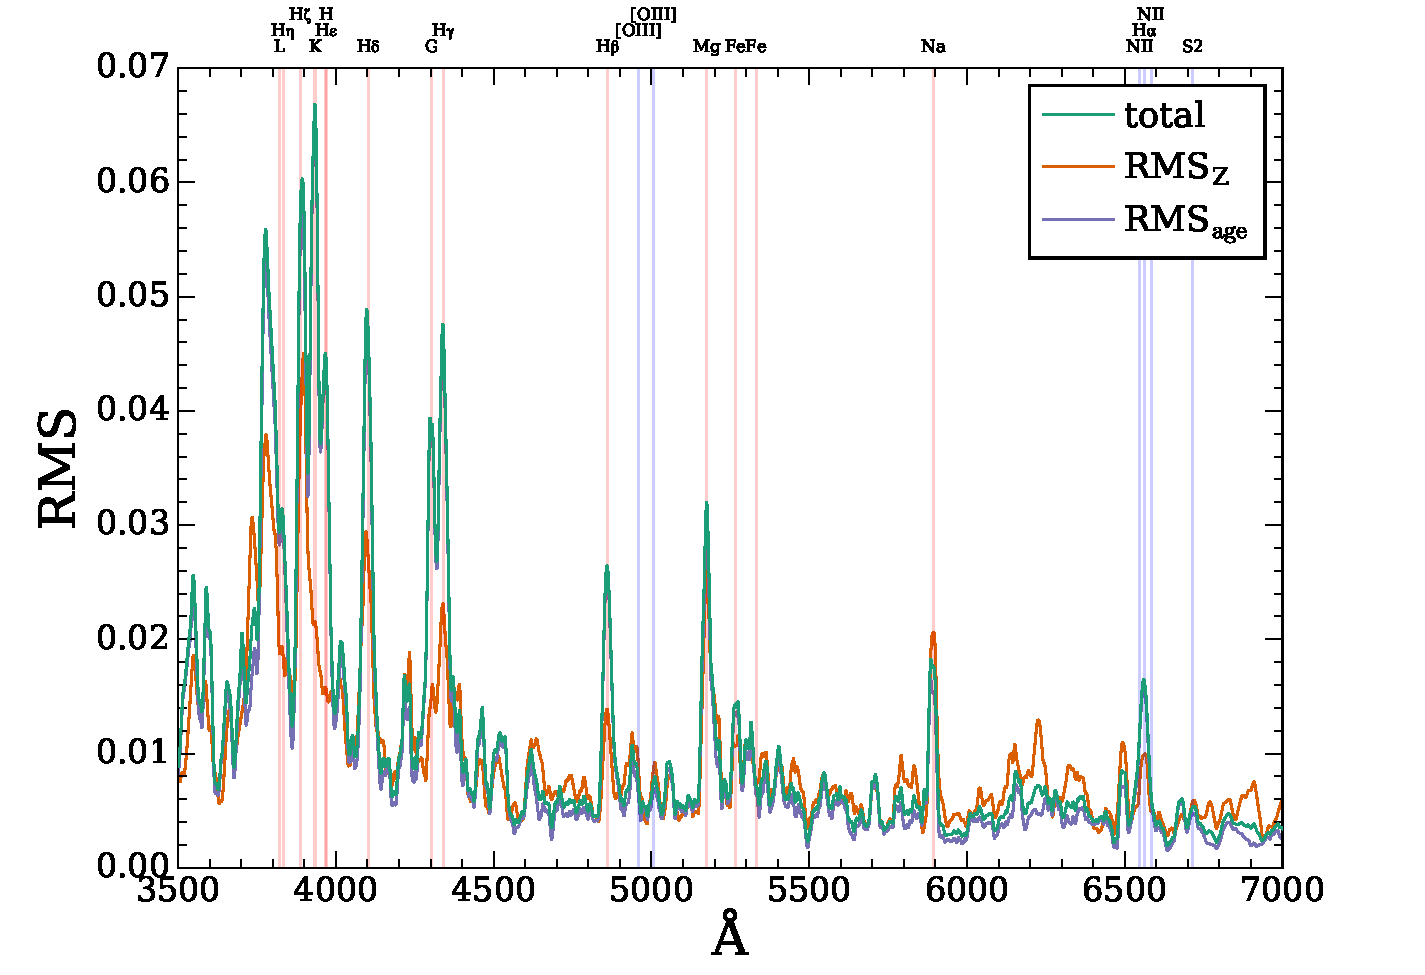
\includegraphics[width=\columnwidth]{891_2/figs/RMS_spec.pdf}
  \caption[RMS-based $\chi^2$ fitting
    weights]{\fixspacing\label{891_2:fig:RMS_spec}The RMS weighting
    function used to modify our $\chi^2$ fits ($R(\lambda)$ in
    Equation. \ref{891_2:eq:smart_chi}). The total RMS value is
    computed across all metallicities and ages. RMS$_Z$ is computed
    across all metallicities and is sensitive to differences between
    models with different metallicity values. Similarly,
    RMS$_\mathrm{age}$ is computed across all ages and is therefore
    more sensitive to model differences as a function of age.}
    %% The red line is the same as the
    %% green, but computed across all metallicities. The red and green
    %% lines show the quadrature sum of the individual RMS$_Z$ or
    %% RMS$_{age}$ computed across all ages or metallicities,
    %% respectively \textbf{this is almost certainly not clear}. Vertical
    %% lines show important emission (blue) and absorption (red)
    %% features.}
\end{figure}

Figure \ref{891_2:fig:RMS_spec} shows the resulting RMS spectrum along
with important spectral features. In addition to computing the RMS
across all ages and metallicities we also compute RMS spectra across
all ages at each metallicity and vice versa. The ``total'' RMS closely
matches the RMS across age, which suggests that age variations cause
the majority of the difference between different SSPs. There are also
few spectral features that are have a high RMS value in \emph{only}
age or metallicity, which suggests these weights will struggle to
break the age/metallicity degeneracy.

The total RMS spectrum modifies the traditional $\chi^2$ by
\begin{equation}
\label{891_2:eq:smart_chi}
\chi^2 = \sum_{\lambda}\left(\frac{f(\lambda) -
  g(\lambda)}{\sigma(\lambda)}\zeta(\lambda)\right)^2,
\end{equation}
where $f(\lambda)$ and $g(\lambda)$ are the data and model spectra,
respectively, $\sigma(\lambda)$ is the poisson errors on $f(\lambda)$, and
$\zeta(\lambda)$ is the RMS spectrum.

%+++++++++++++
%% {\bf MAB: Discuss how to read the figure since it is almost impossible
%%   to make out the $RMS_{age}$ line. I think you want to say that is is
%%   easiest to make out the ``total'' (green) and Z (orange) curves
%%   which demonsrates that in most cases where there are strong peaks
%%   age variations dominates, particularly below 4500 \AA\. Redward
%%   there are weaker features where Z dominates. However, at every
%%   location where there is a strong peak in RMS both age and Z increase
%%   (except perhaps for Ca HK, which is weird), which already
%%   foreshadows that this weighting scheme is not going to bust the
%%   age-Z degeneracy.}


In addition to modifying our full-spectrum fits, the results shown in
Figure \ref{891_2:fig:RMS_spec} provide insight into the statistically
important differences between model spectra. The Balmer series stands
out as strong indicators of both age and metallicity, but surprisingly
the higher-order Balmer lines (\Hd, \Hg) have more power than \HB and
\Ha. This is important because in the absence of an accurate
correction for Balmer emission (\S\ref{891_2:sec:emission_corr}) these
higher order lines are less likely to be contaminated. Beyond the
Balmer series Na, Fe, Mg, and G-band absorption also have powerful
spikes in the RMS spectrum. Unfortunately the distance to NGC 891
places Na absorption right on top of the NaD sky emission line so it
cannot be used in analysis. 

In many ways the index/equivalent width measurements common to
Astronomy and used in Chapter \ref{chap:891_1} can be thought of as
$\chi^2$ comparisons that are very highly tuned to specific spectral
features and therefore are highly dependent on the stellar physics
that go into producing the models. In this context it comes as no
surprise that the spectral features that differentiate our SSP models
are the same features that have been used extensively in the LICK
system to assign astrophysical parameters to observations of galaxy
and stars.

%+++++++++++++++++
%% {\bf MAB: This is a good discussion. I am trying to think whether it
%%   is surprising that \Hd and \Hg have more variation than \HB and \Ha.
%%   This may be well known, but the point about the emission correction
%%   is a good one. Note NaD also problematic because of ISM within the
%%   external galaxy. Concerning ``a ton of people'' just reference the
%%   Lick system and either give no reference or cite something like
%%   Burstein 1984.}

\begin{figure*}[t]
  \centering
%  \includegraphics[width=\textwidth]{891_2/figs/weight_comp_sys.pdf}
  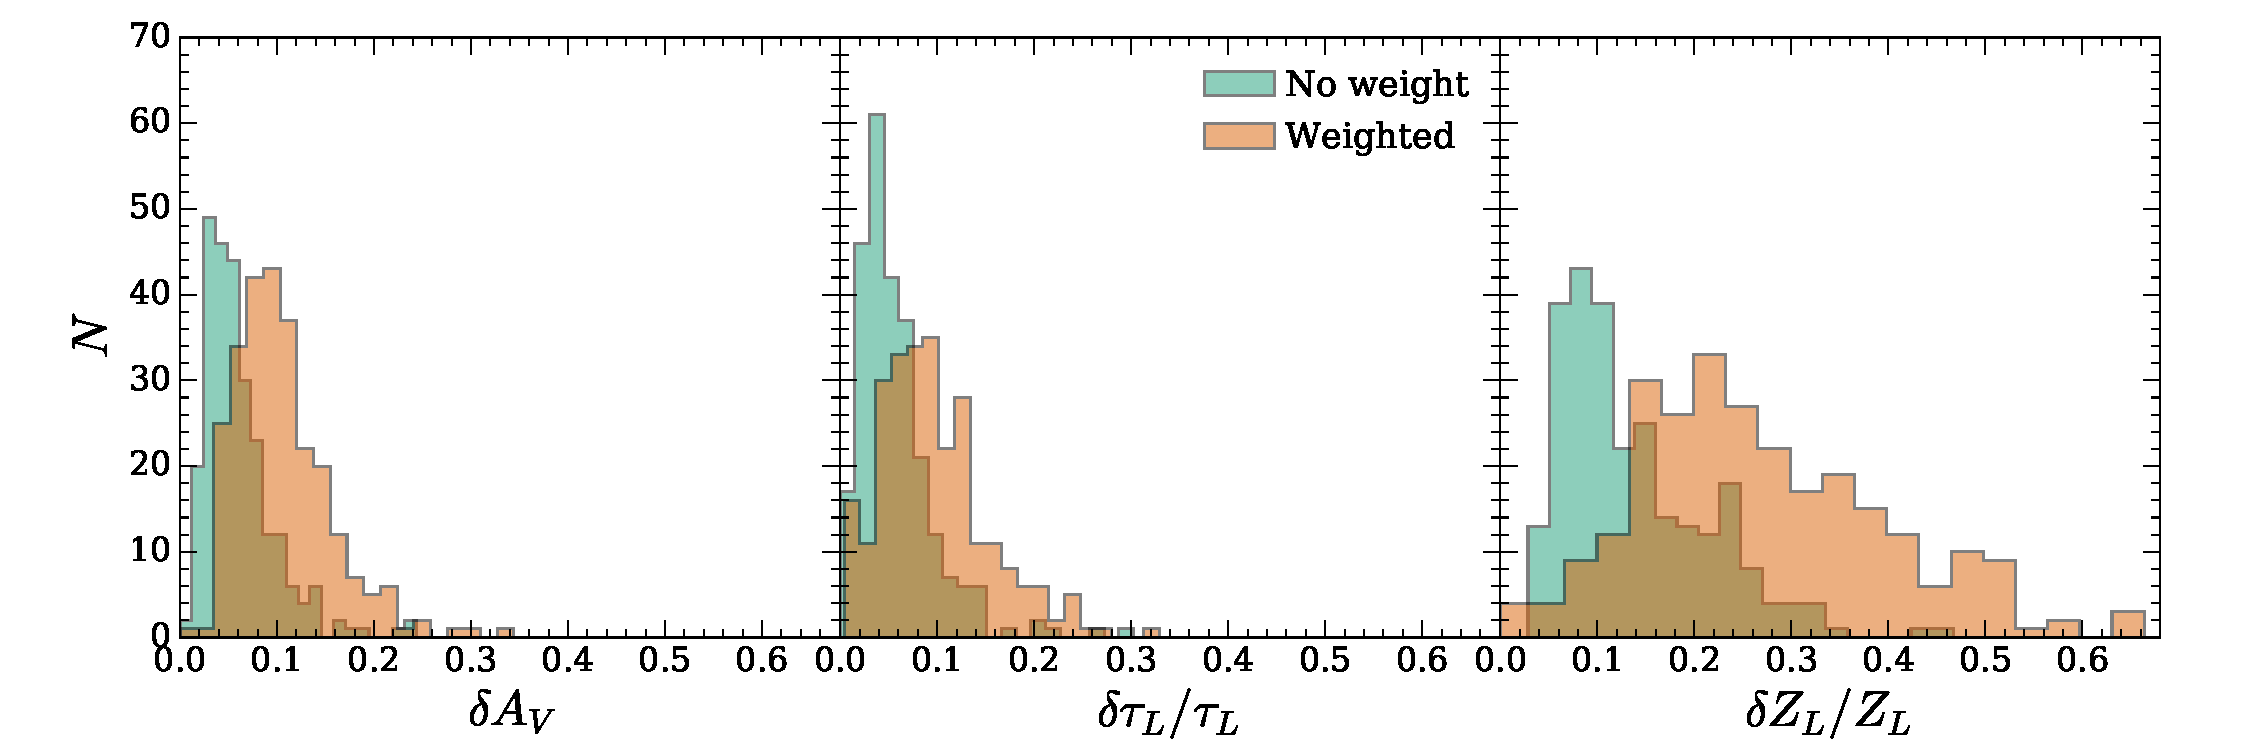
\includegraphics[width=\textwidth]{891_2/figs/weight_comp_hist.pdf}
  \caption[Comparison of uncertainties between weighted and un-weighted
    fits]{\fixspacing\label{891_2:fig:weight_comp}
%% \emph{top:} Derived values of fits
%%     using the weighted $\chi^2$ described in Equation
%%     \ref{891_2:eq:smart_chi} compared to the same values derived using an
%%     un-weighted fit. The dashed lines have a slope of 1. \emph{bottom:}
    Distribution of fitting errors (\S\ref{891_2:sec:fit_err}) for fits
    using un-weighted and weighted $\chi^2$.}
\end{figure*}

%%%%
%ADE: I took out the whole discussion of systematics for now. I think
%it could be interesting, but is not necessary for the argument of why
%we don't use weighted fits.

%% To asses the benefit of using a weighted $\chi^2$ we compare results
%% produced with un-weighted fits to those produced with weighted fits,
%% checking for both systematic differences and the uncertainty distributions
%% of the fits themselves (see \S\ref{891_2:sec:fit_err}). The top
%% panels of Figure \ref{891_2:fig:weight_comp} show the systematic differences
%% between the two schemes. As expected, $A_V$ is highly correlated,
%% indicating that using a weighted $\chi^2$ does not significantly or
%% systematically shift the derived extinction, which speaks to the fact
%% that $A_V$ is mostly driven by the slope of the galaxy SED over a
%% broad wavelength range (although it is also correlated with $\tau_L$,
%% as shown in \S\ref{891_2:sec:fit_err}) and will therefore be relatively
%% insensitive to highly localized changes in $\chi^2$.

%% The middle panel of Figure \ref{891_2:fig:weight_comp} shows that, in many
%% cases, weighted fits find values for $\tau_L$ that are systematically
%% lower than those found via un-weighted fits. This offset is largest
%% for lower values of $\tau_L$, which points to Balmer lines as a likely
%% culprit. In Figure \ref{891_2:fig:RMS_spec} it is clear that the Balmer
%% lines (and in particular \HB, \Hg, and \Hd) are very strong indicators
%% of age and it is likely that the weighted fits increase the fraction
%% of Young SSPs (i.e., lowering the age) to more accurately fit the
%% depth of these lines at the expense of a worse fit in the inter-line
%% continuum where the $\chi^2$ weights are small. 

%% {\bf MAB: This continues to be good discussion. I was wondering if it
%%   is possible to {\it show} your plausible conjecture that the
%%   inter-line regions are not fit a well in the weighted fits, e.g.,
%%   mean spectral residuals. I have a different interpretation of the
%%   middle panel. To my eye the correlation is excellent at the earliest
%%   and youngest ages. At intermediate ages, which just happens to be
%%   where our DFK are probably too coarse, ther is significantly more
%%   scatter.  I don't know what this is telling us but it would be nice
%%   to identify a group of outliers and again compare the mean spectral
%%   residuals between the two classes of fits.}

%% The right panel of Figure \ref{891_2:fig:weight_comp} indicates systematic
%% offsets in $Z_L$ caused by using a weighted $\chi^2$. In particular at
%% low metallicities, as reckoned by the weighted fits, the weighted fits
%% produce systematically lower values while at high metallicities (again
%% weighted by the weighted fit) the weighted fits produce systematically
%% higher values. Many of the strong metallicity indicators shown in
%% Figure \ref{891_2:fig:RMS_spec} have relatively weak amplitudes when
%% compared the uncertainty in the flux values (i.e., they have a low
%% signal to noise) and by increasing the weight in these regions we are
%% possibly pushing $\chi^2$ beyond the limits of our uncertainty. When
%% the signal in one of these metal lines is strong (i.e. high
%% metallicity) the weighted fit will attempt to accurately match the
%% depth of the feature by increasing the fraction of metal-rich SSPs
%% beyond what we be allowed by an un-weighted fit (which is relatively
%% more constrained by the ``featureless'' continuum). When there is very
%% little signal in the metal lines, however, the weighted fits are
%% forced to avoid a small level of absorption on the level of the flux
%% uncertainty that would otherwise be allowed in the un-weighted
%% fits. In other words, in the weighted fits weak metal absorption lines
%% cannot ``hide in the noise'' and therefore a lower total metallicity
%% is needed.

%% {\bf MAB: This needs to be articulated more clearly: ``we are possibly
%%   pushing $\chi^2$ beyond the limits of our uncertainty.'' I didn't
%%   follow your subsequent examples. Even with the weights, there are
%%   many lines. Noise will not make all of them artificially high or
%%   low. So why the systematic difference? And which do you think is
%% right?}

To asses the benefit of using a weighted $\chi^2$ we compare fitting
uncertainties (\S\ref{891_2:sec:fit_err}) produced by un-weighted fits to
those produced with weighted fits and find, somewhat surprisingly,
that a weighted $\chi^2$ produces significantly less precise fits.
Figure \ref{891_2:fig:weight_comp} shows that for all parameters of interest
the distribution of fit uncertainties is larger for weighted fits than
for un-weighted fits, often by a factor of $>$ 2. This level of
uncertainty is unacceptable and it is clear that weighted fits
\emph{do not} improve our ability to understand NGC 891. They are
therefore abandoned for the remainder of this work. We would like to
note, however, that these tests are in no way an exhaustive
exploration of the general concept of weighted $\chi^2$ and we
encourage future research in this topic.

%-------------------
%% {\bf MAB: We are going to need to do a better job here justifying this
%%   section. I want us to keep it in for the final paper; it should
%%   definiely be in the thesis, even as is.  For the paper we need more
%%   work.

%% The key issue that I think we have not fleshed out enough
%% is consideration of accuracy. What we have shown definitively is
%% that weighting reduces precision. This is surprising because we
%% thought we were up-weighting the regions where the astrophysical variance 
%% (which is our ``signal'') was largest. In the above paragraph you 
%% are starting to get at the key issue, namely with statements about
%% systematic differences (could be related to different accuracy) relative
%% to random errors. We need to do two things.

%% (1) Quantify and illustrate the level of systematics vs increased
%% random error (we've only done the latter).

%% How do the projections of $Z_L$, $\tau_L$ and $A_V$ compare for the
%% two fitting methods? Can we say one looks more astrophysically
%% plausible than another? Even if no, this is important to know. Let's
%% make the plots and look at them. Maybe one set w/ two colors for
%% points -- unless we also want to look at height and radius trends.

%% (2) Identify ways to assess if we think one method is more accurate
%% (in the mean) than the other.

%% I would start by looking at the mean residuals for the different fit
%% cases.  As noted above, we may want to do this for subsets of the data
%% where systematics in age and Z are most pronounced. It would be nice
%% to see of the scatter is different in the up-weighted vs down-weighted
%% areas, but I think the key is to identify if one fitting method
%% systematiclly over or under-estimates features or continuum.

%% Where I think we should be going with (1) and (2): While the weighted
%% fits may be noiser, it may be that they are more accurate in the
%% mean. If so this mean provides a possible systematic correction we
%% could apply to the un-weighted fits IF we thought there was some
%% reasonable way to do this. (It will depend on what we find in (1)
%% above.) If we cannot conclude that one fitting method vs the other is
%% plausibly more accurate, then at least we have quantified one
%% assessment of potential systematics in our fitting. That alone
%% justifies the section. In short, you are on the right track; we just
%% need to push it the final step.

%% Wording: ``quantities with larger systematic offsets (i.e., $Z_L$)
%% also have larger fit uncertainty, which dilutes the magnitude of the
%% offset.'' No, it doesn't dilute the magnitude of the offset but its
%% significance.

%% Last two sentences should be revised based on our additional work
%% and/or specific recommendations for future effort (for starters: what
%% we would like to do if we have time.}

%% On the other hand, a full-spectrum fit like that
%% described in \S\ref{891_2:sec:SSP_method} more accurately captures the SED
%% of a galaxy at the expense of strong constraints on the detailed
%% astrophysics. Our RMS-weighted full-spectrum fitting is designed to
%% occupy a middle ground between these two methods. With it we are able
%% to leverage our astrophysical knowledge to focus in on key regions
%% while at the same time fitting all of these regions at once along with
%% the continuum shape. It pretty much rules.


\section{Uncertainties}
\label{891_2:sec:uncertainty}

Uncertainties in our derived parameters ($\tau_L$, $Z_L$, $A_V$) come
from a number of sources: the precision and accuracy of the data
(e.g., random errors and flux calibration, respectively); degeneracies
between age, metallicity, and extinction as coupled in the model
parameters; and systematic uncertainty in our interpretation of the
results of the fit. In the context of our DFK basis set, the latter
consists of the assignment of the effective age of each template,
which then propagates into the mass- or light-weighted mean age and
metallicity.  In this section we quantify the magnitude of these
uncertainties, first looking at the coupling between random errors in
the data and covariance in age, metallicity, and extinction.
 

\subsection{Stochastic Uncertainty and Covariance}
\label{891_2:sec:fit_err}

\begin{figure*}
  \centering
  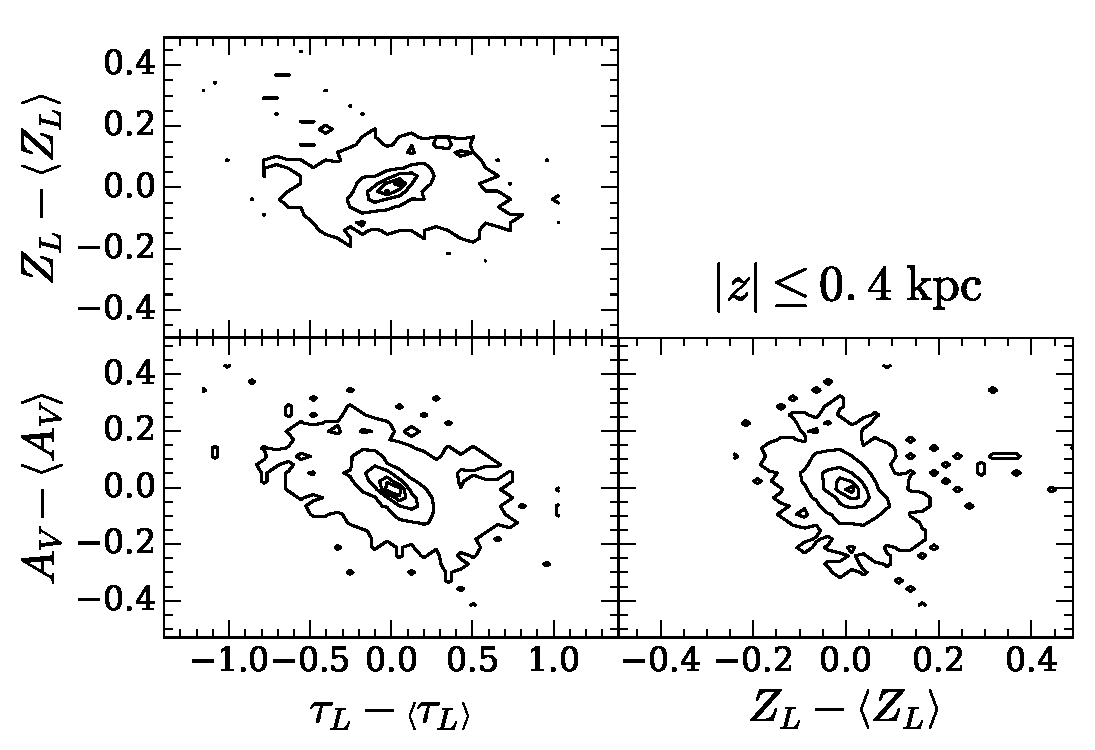
\includegraphics[width=0.48\textwidth]{891_2/figs/MC_covarcont_below.pdf}
  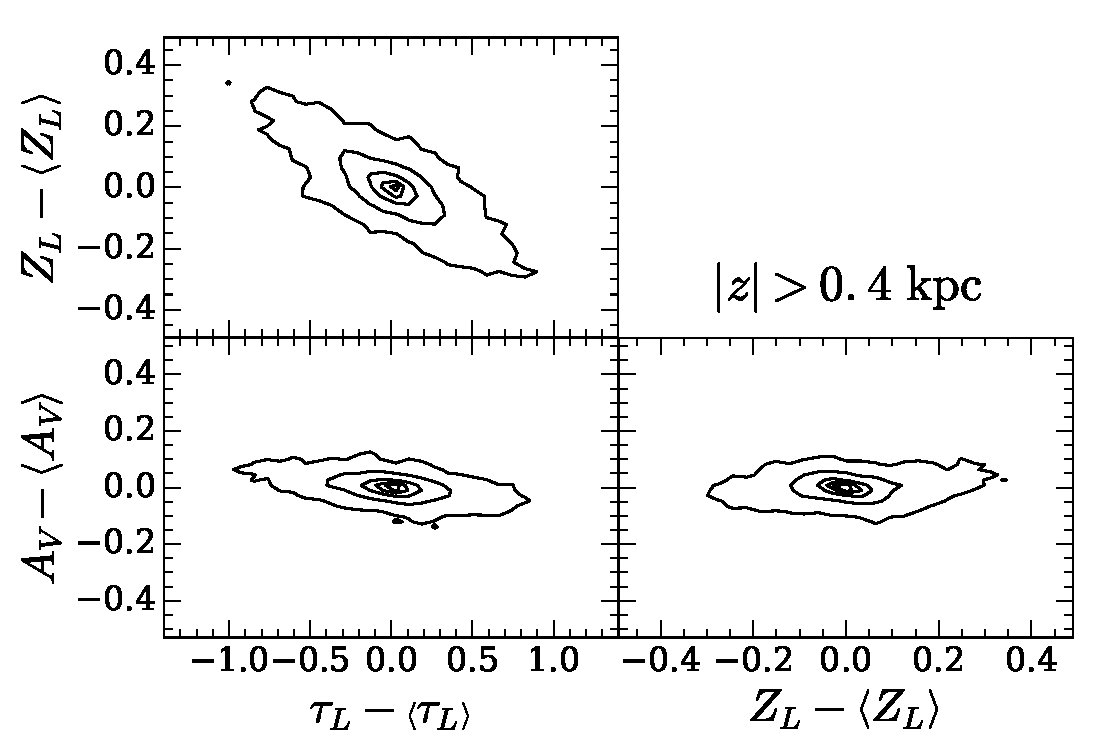
\includegraphics[width=0.48\textwidth]{891_2/figs/MC_covarcont_above.pdf}
  \caption[Covariance between uncertainties in $\tau_L$, $Z_L$, and
    $A_V$]{\fixspacing\label{891_2:fig:MC_covar}Derived parameters for
    all iterations of the Monte Carlo noise perturbations for all
    apertures. To remove real differences in values between apertures
    the values for each aperture are zeroed to the mean of the 100
    noise perturbations. \emph{left:} Data for apertures below
    \val{0.4}{kpc}. \emph{right:} Data for apertures above
    \val{0.4}{kpc}. The contour levels are 0.5\%, 10\%, 40\%, 70\%,
    and 90\%.}
\end{figure*}

Stochastic uncertainty in ($\tau_L$, $Z_L$, $A_V$) that arises during
full spectral fitting is driven by two effects: uncertainty in the
true shape of our galaxy SED and degeneracies between age, extinction,
and metallicity. The uncertainty of the SED of NGC 891 is already
quantified, it is exactly the error spectrum computed as part of the
data reduction described in \ref{chap:891_1} and accounts for
uncertainty in wavelength calibration, sky subtraction, and flux
calibration.

%+++++++++++++++++
%% {\bf MAB: above par. may be a bit redundant with intro par. for the
%%   section, but I would keep the intro par. as is and modify here
%%   accordingly. Pay attention to your use of the term ``shape of the
%%   galaxy data.'' I think you might mean the ``shape of the spectral
%%   energy distribution'' but it is important to be clear if you mean
%%   low or high frequency. I think low frequency is relevant in terms of
%%   flux calibration errors and couples most directly to uncertainties
%%   in age and extinction. The higher-frequency errors associated with
%%   shot noise or sky-subtraction are more likely to impact age and
%%   metallicity.  It might be useful to make these distinctions and
%%   discuss here. Also you should note if flux-cal uncertainties have or
%%   have not been included in the analysis, and if not, why not, or why
%%   we don't care.}

Degeneracies in fit parameters are generally well understood, but more
difficult to quantify. The primary degeneracy in our fits is the well
known age/metallicity degeneracy \citep[see, for
  example,][]{Oconnel76,Aaronson78,Worthey94,dePaz02}, whereby a mix
of younger, more metal-rich populations can be spectrally
indistinguishable from a mix of older, more metal-poor
populations. This correlation is especially relevant to our work given
our attempt to simultaneously fit SSPs with multiple metallicities and
ages.

Secondary degeneracies exist between extinction and both age and
metallicity, the amplitudes of which are dependent on the overall age
of the model spectrum. In models with a high fraction of young SSPs
extinction is strongly correlated with age. This is due to the fact
that the stars dominating the blue-visible portion of the spectrum in
these populations are so hot that any metals present will be
sufficiently ionized that their contribution to stellar atmospheric
opacity is negligible. Thus the only way to change the slope of the
continuum is to either vary age or attenuation.

%% Furthermore, in the absence of extinction
%% older populations are redder due to cooler temperatures and increased
%% line blanketing, but younger populations can be extincted to match,
%% over large wavelength ranges, the general continuum shape of old
%% populations. For single populations this effect is minimal; absorption
%% lines can differentiate different population ages independent of
%% continuum shape, but in composite galaxy spectra made from the
%% superposition of many SSPs (i.e., our spectral fits) the amount of
%% light coming from old populations can be decreased (although not
%% eliminated) be increasing the extinction.

In intermediate-aged populations metal absorption lines make up a key
component of the opacity in stellar atmospheres and a higher
concentration of metals absorption lines will ``redden'' the spectrum
through increased line-blanketing at bluer wavelengths in the stellar
photospheres \citep[see, e.g., Figure 4 in ][]{Vazdekis10}. In this
regime there is a strong negative correlation between metallicity and
extinction because the model spectrum can be reddened by increasing
the strength of these metal lines. The left panel of Figure
\ref{891_2:fig:MC_covar} shows this effect in the ($A_V$, $Z_L$)
plane. As we will see in \S\ref{891_2:sec:SFH}, below \val{0.4}{kpc}
most of the measured light comes from intermediate populations where
the correlation between $A_V$ and $Z_L$ is strongest.

There is a limit to this effect, however; the very oldest SSPs are
cool enough that there is significant metal-line reddening regardless
of the overall metallicity (at least within the range of metallicities
considered here) and increasing the total metallicity will not
appreciably change the shape of the continuum. This effect can be seen
in the right panel of Figure \ref{891_2:fig:MC_covar}; there is very little
correlation between $Z_L$ and $A_V$ in regions dominated by the Old
DFK bin.

%% A secondary degeneracy exists between metallicity and extinction. A
%% pristine spectrum can be reddened either through the presense of
%% wavelength dependent attenuation (i.e., classical reddening) or
%% through the addition of strong metal absorprion lines. Importantly,
%% there is an age dependence to this effect; young populations are so
%% hot that any metals present will be fully ionized and therefore won't
%% contribute to the total opacity so the slope of the continuum is only
%% weakly dependent on metallicity. In intermediate-aged and old
%% populations, on the other hand, metal absorption lines make up a key
%% component of the opacity in stellar atmospheres and a higher
%% concentration of metals will ``redden'' the spectrum by removing
%% black-body continuum from strong absorption features blueward of
%% \val{\asim 5000}{\AA} (e.g., Fe, Mg, G-band, Ca). %Figure here?

%++++++++++++++++++++++++
%% {\bf MAB: You have everything right here, but the paragraph needs some
%%   re-arrangement. I would lead by saying that age and Z both play off
%%   $A_V$, but the relative importance depends on age. I.e., at young
%%   ages (probably $<$ 0.5-1 Gyr) age reigns supreme in wagging $A_V$
%%   and vice versa. For older ages, it's Z vs $A_V$. I think this will
%%   set the stage for your covariance plots latter. ``through the
%%   addition of strong metal absorprion lines'' should become ``through
%%   increased line-blanketing in stellar photospheres at bluer
%%   wavelengths due to strengthened metal absorption lines.'' You
%%   actually say this latter. Like I said, the words are there! I
%%   wouldn't call out the strong lines in terms of the line-blanketing
%%   effect, but rather the forest of weak lines that supreses the real
%%   continuum to a redder pseudo-continuum level. I think Conroy shows
%%   this pseudo-continuum concept in his review, to which you could
%%   refer.}

%% Finally, there can be degeneracies between age and extinction. In the
%% absence of extinction older populations are redder due to cooler
%% temperatures and increased metal absorption, but younger populations
%% can be extincted to match, over large wavelength ranges, the general
%% continuum shape of old populations. For single populations this effect
%% is minimal; absorption lines can differentiate different population
%% ages independent of continuum shape, but in composite galaxy spectra
%% made from the superposition of many SSPs (i.e., our spectral fits) the
%% amount of light coming from old populations can be decreased (although
%% not eliminated) be increasing the extinction.

%++++++++++++++++++
%% {\bf MAB: I think you can wrap this paragraph into the previous one
%%   along the lines noted. Also, since we've mentioned that there is an
%%   age-Z degeneracy, it is probably worth stating that the coarse age
%%   differentiation for when $A_V$ is degenerate with age vs when it is
%%   more degenerate with $Z$ is sufficiently large that the age-$Z$
%%   degeneracy is no significant in altering the discussion.}

To quantify uncertainties caused by these effects we construct a set
of 100 Monte Carlo iterations of each galaxy spectrum. For each
iteration the galaxy flux at a specific wavelength, $f(\lambda)$, is
perturbed by an amount randomly chosen from a normally distributed set
of values with a width equal to the error spectrum computed during
data reduction. Thus, the $k$th Monte Carlo spectrum is $f_k'(\lambda)
= f(\lambda) + r(e(\lambda))$, where $r(\sigma)$ represents a normal
distribution with width $\sigma$ and $e(\lambda)$ is the galaxy error
spectrum. Each of the $f_k'(\lambda)$ spectra are then fit with the
identical method and SSP library (\S\ref{891_2:sec:final_SSP}). The ``true''
value of the fit parameters is then taken to be the mean over all 100
iterations while the total fit uncertainty (i.e., stochastic plus
degeneracies) is defined by an ellipse in ($\tau_L$,$Z_L$,$A_V$) space
that contains 68\% of all Monte Carlo iterations (i.e., a 68\%
phase-space confidence interval). The reported uncertainties for each
individual parameter are the projection of the limits of this ellipse
onto the specific parameter.

The decision to perform Monte Carlo perturbations on our data rather
than the best fit model is similar to the approach taken by PIPE3D
\citep{Sanchez16}, and we feel it yields important
information. Namely, it allows us to quantify how any systematic
differences between our data and the models couple with random
uncertainties in the data. In other words, it fully encapsulates all
sources of uncertainty that affect the final fits.

%+++++++++++++++++
%% {\bf MAB: You want to say something about the approach of using the
%%   data instead of the models for the MC here. (a) This requires you
%%   smooth the data and models (say how much); but (b) it allows you to
%%   determine how any systematics differences between data and models
%%   couples to random errors in the data -- somthing that can't be done
%%   from doing MCs of the models. And just so we aren't attacked by the
%%   Spanish Armada....I think there is a reference to Sanchez who does
%%   the same. We must reference if so.}

Figure \ref{891_2:fig:MC_covar} shows the result of the Monte Carlo
runs. In the majority of apertures our quantities of interest show the
expected degeneracies discussed above (negative age/metallicity
correlation, negative age/extinction correlation, and negative
metallicity/extinction correlation) however there are large group of
apertures that exhibit a \emph{positive} correlation between age and
metallicity (i.e., increasing the metallicity leads to fits that have
older ages). This seemingly backward trend is reasonable (and
expected) in the context of how the reddening affects different aged
populations. Apertures with a positive age/metallicity relation are
concentrated below the age break at \val{0.4}{kpc} (Chapter
\ref{chap:891_1}) and therefore have a high fraction of total flux
contributed by young SSPs (although, importantly, I2 and Old
populations still contribute the majority of the light, a la
\S\ref{891_2:sec:SFH}). As discussed above, young SSPs have a
continuum shape that is only weakly dependent on metallicity, so
reddening is achieved by increasing $A_V$. Thus, as the fraction of
Young SSPs increases more extinction is needed to redden the models to
the level of the data. This increase in total extinction (for a given
aperture) then requires the I2 and Old SSPs to have lower
metallicities to counteract the extinction-induced reddening. This
decreases the total metallicity, $Z_L$, because (as shown in
\S\ref{891_2:sec:SFH}) I2 and Old SSPs still contribute the majority
of the light at all points in the galaxy. Thus, the positive
age/metallicity correlation at small heights is the result of the fact
that metallicity is a weighted average that is mostly dominated by
older SSPs, and that a single extinction value, $A_V$, is applied to
all SSPs in a particular fit.

%% {\bf MAB: I am not sure I buy your conclusion, so I recommend we redo
%%   this starting with the parts we do agree on, and then get to the
%%   more challenging bits. So start with a first-order description of
%%   Fig \ref{891_2:fig:MC_covar}, as follows:

%% $\bullet$ $A_V$-age: negative at all heights; stronger at lower $z$

%% $\bullet$ $A_V$-Z: negative at hi-$z$; flat at low-$z$.

%% $\bullet$ Z-age: more weakly correlated at low $z$, with a hint that
%%   it is a postive correlation; strongly negative correlation at
%%   hi-$z$.  Concerning the hint, see comment in figure caption. This is
%%   likely more than a hint but you need to discuss significance of
%%   contour levels.

%% Then I would turn first to discuss the r.h. panels for $z>0.4$ kpc for
%% the older pops and describe how it makes sense. The big deal is
%% age-metallicity; well known. But note there is a little degeneracy in
%% AV and age, although apparently none between AV and Z which refutes
%% our line-blanketing spit-balling earlier in the text.

%% Then I would turn to the less-intuitive situation at low heights where
%% ages are lower. (You should either or both hark back to Paper I to
%% quote what you think are the characteristic ages in the $z<$0.4 kpc
%% and $z>0.4$ kpc bins, or compute the average from later sections in
%% the paper.  Note in text or caption.)

%% Here's what I don't buy (yet):

%% ``...young SSPs have a continuum shape that is only weakly dependent
%% on metallicity, so reddening is achieved by increasing $A_V$. This
%% increase in total extinction (for a given aperture) requires older
%% SSPs to have lower metallicities to counteract the extinction-induced
%% reddening. Thus, the positive age/metallicity correlation at small
%% heights is the result of the fact that metallicity is a weighted
%% average that is mostly dominated by older SSPs, and that a single
%% extinction value, $A_V$, is applied to all SSPs in a particular fit.''

%% The underlying premise is this:

%% ``metallicity is a weighted average that is mostly dominated by older
%% SSPs''

%% But it is not correct. The metallicity is light-weighted, so if the
%% population is young $Z_L$ is a measure of the metallicity of the young
%% stars. 

%% Here's my theory:

%% ``because young SSPs have a continuum shape that is only weakly
%% dependent on metallicity, variations in the stellar population age and
%% $A_V$ both serve to be the primary ways to redden the continuum shape.
%% Consequently these model parameters are strongly negatively
%% correlated.  When increases in model age overly serve to fit the
%% reddened continuum, to compensate for the increased metal line
%% strength one might expect the model metallicy to diminish. In fact the
%% opposite is seen, i.e. surprisingly age and metallicity are {\it
%%   positively} correlated. We believe this is an artifact of having
%% adopted a constant extinction value for all age templates. A more
%% realistic model would tend to apply more extinction to the younger
%% populations. As a consequence, when the ratio of young to old stars is
%% over-estimated, this diminishes the model metal-line equivalent
%% widths, and to compensate the model metallicity must increase.''

%% If this is what you mean, then it is just that your wording is
%% confusing or unclear.

%% }  
 
\begin{figure*}
  \centering
  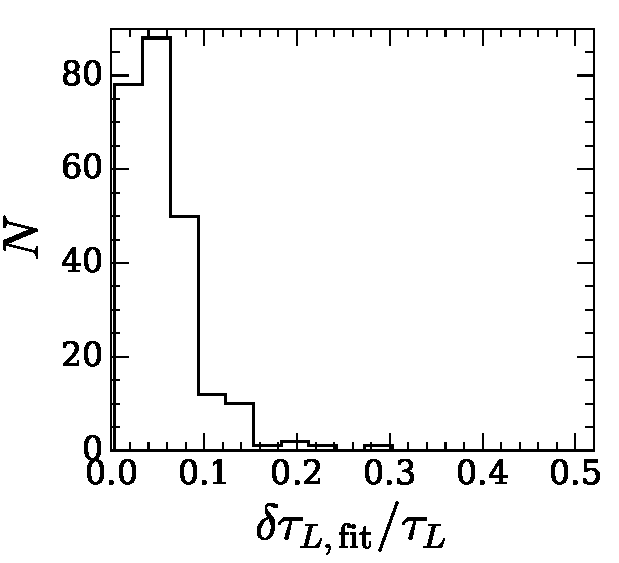
\includegraphics[width=0.31\textwidth]{891_2/figs/fit_uncertainty_MLWA.pdf}
  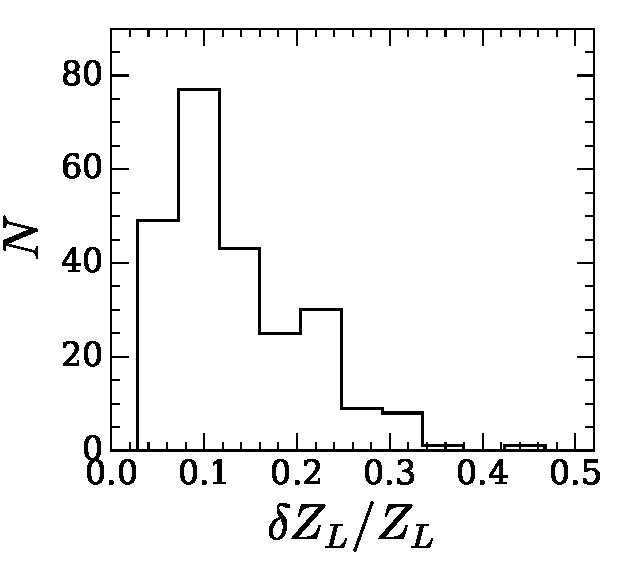
\includegraphics[width=0.31\textwidth]{891_2/figs/fit_uncertainty_MLWZ.pdf}
  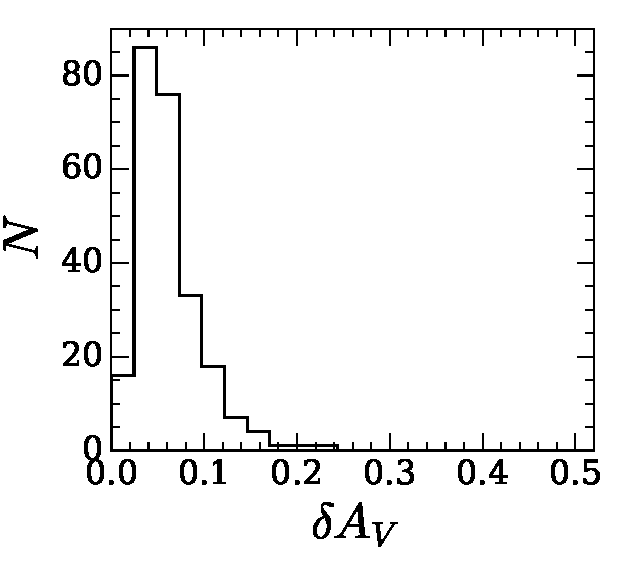
\includegraphics[width=0.31\textwidth]{891_2/figs/fit_uncertainty_TAUV.pdf}
  \caption[Distributions of fit uncertainties in $\tau_L$, $Z_L$,
    $A_V$]{\fixspacing\label{891_2:fig:fit_err_hist}Distribution of
    parameter uncertainties in age, metallicity, and extinction
    derived from full spectral fitting.  The uncertainties are 68\%
    confidence limits on all three parameters simultaneously based on
    the Monte Carlo perturbations described above.}
\end{figure*}

The fact that a purely random perturbation of our data results in fits
that clearly show the expected astrophysical degeneracies indicates
that these degeneracies are primary source of fitting uncertainty. In
other words, uncertainty in our SSP fits is driven mainly by
similarities between different model SSPs; random flux errors in a
given wavelength channel are only a secondary source of fitting
uncertainty.

%% {\bf MAB: The hard question then is why did we bin to such high
%% S/N?}  

%% ADE comment: The binning was based on theory. Here is the
%% reality. Better to be in this case than a situation where data
%% uncertainty drives our total uncertainty.

We compute total fitting uncertainty using the method described above
separately for each aperture. The values thus derived constitute all
sources uncertainty that arise from the simultaneous measurement of
the three parameters. Figure \ref{891_2:fig:fit_err_hist} shows the
distribution of uncertainties in age, metallicity, and
extinction. Fitting uncertainties are on the order of 5\% for most
apertures, but the distribution of uncertainty in metallicity is
broader than either $\tau_L$ or $A_V$ and can reach \asim 30\% in the
worst cases.

%+++++++++++++++
%% {\bf MAB: You want to emphasize that ``total'' here includes the
%%   degeneracies, i.e., these are not marginalized, but are the
%%   uncertainties in simultaneous measurement of all three parameters.

%--------------
%% {\bf $>>>$ How do these uncertainties compare to what you predicited in
%%   Paper I?}

\subsection{Systematic Uncertainty in DFK Ages}
\label{891_2:sec:sys_err}

Computing a weighted age for a superposition of model SSPs requires
assigning a specific age to each individual SSP, which, in turn,
requires making an assumption about the star formation history (SFH)
across the range of ages spanned by the SSP age bin (see Table
\ref{891_2:tab:dfk}). Different SFHs have minimal impact on the youngest
SSPs due to their narrow age range, but the oldest SSPs span a range
of over \val{7}{Gyr} and thus the age assigned to this bin can vary by
the same magnitude, depending on the assumed SFH. Because of this, the
choice of SFH creates systematic uncertainty in the computed value of
$\tau_L$. This uncertainty is primarily a consequence of the fact that
old stellar spectra are essentially constant over a large age
range. In other words, these old populations do not provide enough
information in their spectral shape to yield precisely defined ages.

%+++++++++++++++++
%% {\bf MAB: Here I think it is worth reminding the reader that this
%%   problem of the older DFK bins isn't due to a bad choice on our or
%%   M15's part, but rather that the width of the bins reflects our
%%   ignorance, or rather, where we do not have information.}

To quantify this systematic uncertainty we compute $\tau_L$ as derived
from 100 Monte Carlo SFHs. For each Monte Carlo iteration we assign
each DFK bin an age that is randomly selected from a uniform
distribution bounded by the limits of the age bin given in Table
\ref{891_2:tab:dfk}. These ages correspond to $t_i$ in Equation
\ref{891_2:eq:MLWA}, which allows us to compute a different $\tau_L$ for
each iteration. It is important to note that $t_i$ is the only
quantity that changes between iterations; the specific SSP weights
($W_{L,i,j}$) are held constant at their best fit values. The standard
deviation of $\tau_L$ across all 100 Monte Carlo iterations quantifies
the systematic uncertainty that results from assuming a SFH.

By choosing $t_i$ completely randomly from within the corresponding age
bin we allow completely unconstrained SFHs, which makes our computed
uncertainty an upper limit. The drawback of this approach is an
almost-certain over estimation of the true systematic uncertainty, but
the benefit is that we are not required to make assumptions about the
general form of the SFH. In this way, our computation
captures not only our lack of knowledge about the specific shape of
SFH, but also our lack of knowledge about the general form of SFH
(e.g., bursty versus smooth).

\begin{figure}
  \centering
  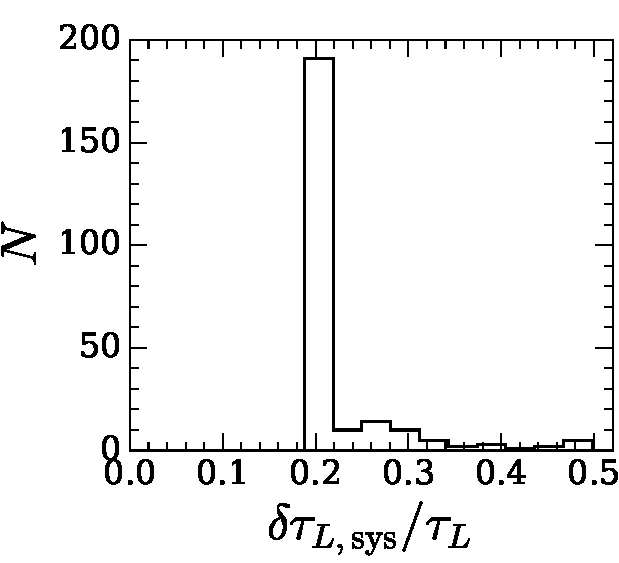
\includegraphics[width=0.45\textwidth]{891_2/figs/sys_uncertainty_hist.pdf}
  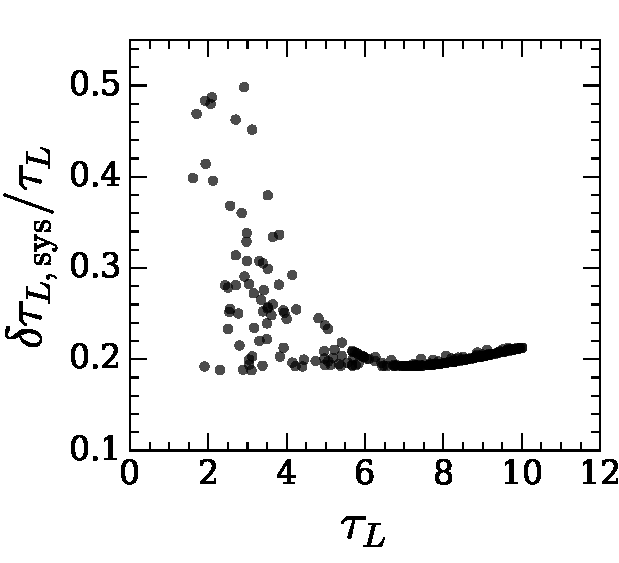
\includegraphics[width=0.45\textwidth]{891_2/figs/sys_uncertainty.pdf}
  \caption[Distribution of systematic uncertainties in
    $\tau_L$]{\fixspacing\label{891_2:fig:sys_err}\emph{top:}
    Distribution of systematic uncertainty that arises from assuming a
    star formation history. The uncertainties are the standard
    deviation of 100 values derived from a random assignment of ages
    to the SSP basis set. \emph{bottom:} The same systematic
    uncertainties as a function of $\tau_L$.}
\end{figure}

The top panel Figure \ref{891_2:fig:sys_err} shows the distribution of
systematic uncertainties in $\tau_L$. In the majority of our apertures
this uncertainty is \asim 20\%, but there is a tail with high
fractional uncertainties that extends up to 50\%, which, as shown in
the bottom panel, comes from apertures with $\tau_L < \val{\asim
  5}{Gyr}$. As we will see in \S\ref{891_2:sec:SFH} I2 and O
populations make up the largest contributions to the total light in
all apertures, even those with a significant fraction of younger
populations and it is these older populations that have the largest
systematic uncertainty due the large range of ages they
represent. Thus in all apertures the systematic uncertainty is
dominated by the presence of old populations. Figure
\ref{891_2:fig:MLWA_sys_err} shows these uncertainties in the context
of the age gradients presented in \S\ref{891_2:sec:rz}; the magnitude
of these uncertainties still allows us to determine broad, smooth
trends over large ranges in height, but it becomes difficult to make
statements about the detailed age structure of NGC 891.

%% given the magnitude of these uncertainties it is
%% difficult to make strong statements on the detailed structure and
%% trends in age or any other measured quantity.

%++++++++++++++
%% {\bf MAB: Spell out the computation for me. You have 100 sets
%% of DFK ages. For each aperture you take the best fit DFK weights,
%% compute 100 values of $\tau_L$, and then take the mean
%% and standard deviation of these values. That ratio is plotted in the figure.}

\begin{figure}
  \centering
  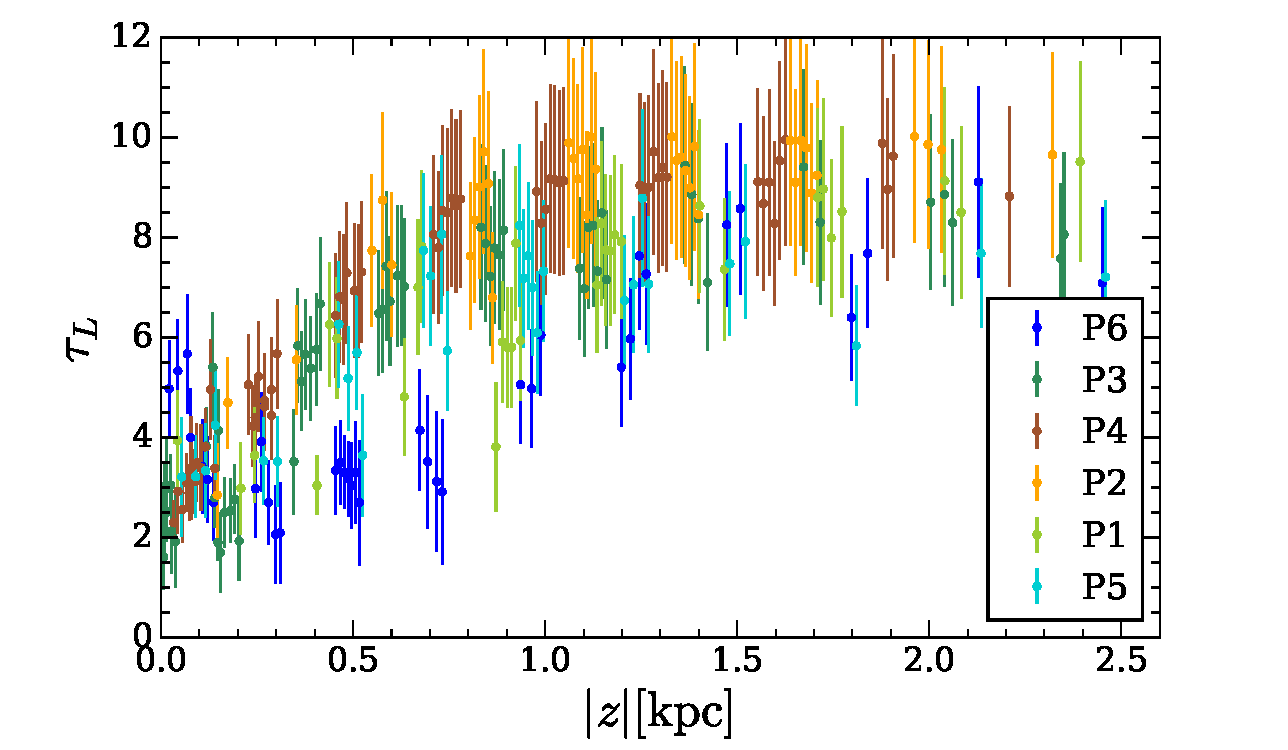
\includegraphics[width=\columnwidth]{891_2/figs/MLWA_sys_err.pdf}
  \caption[Systematic $\tau_L$ uncertainties in relation to our data]
          {\fixspacing\label{891_2:fig:MLWA_sys_err}$\tau_L$ as a
            function of height above the midplane showing the
            magnitude of the systematic uncertainties that arise from
            assuming a star formation history.}
\end{figure}

Despite this bleak picture, we urge the reader to take solace in the
fact that the systematic uncertainties presented above are an extreme
upper limit and ignore NGC 891 as a coherent galaxy. In other words,
it is unreasonable to assume that the SFH within NGC 891 varies on
time scales greater than a dynamical timescale (\val{\asim
  1}{Gyr}). Thus, when assessing trends in $\tau_L$, $Z_L$, or $A_V$ we
can say with confidence that points near each other in phase space
likely come from the same underlying population(s), despite the large
systematic uncertainties. It is only on large physical and time scales
that these uncertainties become relevant. Furthermore, in
\S\ref{891_2:sec:SFH} we find evidence that the general form of SFH is
mostly invariant over the portion of NGC 891 we measure. For these
reasons we choose not to include systematic uncertainties in the final
results shown in \S\ref{891_2:sec:results}, where we draw conclusions about
the detailed, small-scale structure of NGC 891. If we were to compare
the global results for NGC 891 presented here to other galaxies with
potentially different SFH then the systematic uncertainties would be
relevant.

%------------------
%% {\bf MAB: I agree with everything you say here, but I would word it
%%   differently, emphasizing earlier that Figure \ref{891_2:fig:sys_err} is
%%   the worst case of the worst case.}

%% ADE comment. Not sure what you mean here, I think it does a good
%% job as it is.


\section{Results}
\label{891_2:sec:results}

\subsection{Age and Metallicity}
\label{891_2:sec:tZ}

The analysis methods described above allow us to measure $\tau_L$ and
$Z_L$ as a function of galactic radius and height. This parameter
space can yield powerful insights into the history and formation of
NGC 891, but first it is useful to examine the distribution of these
parameters on a galactic scale, as shown in Figure
\ref{891_2:fig:tauZ_hist}. In the left panel we see a multi-modal
distribution of $\tau_L$ that suggests multiple epochs of star
formation in NGC 891. We assign these epochs 4 rough age bins: the
most recent epoch of star formation at $\tau_L < \val{4.3}{Gyr}$, a
somewhat quiescent and relatively constant era of star formation from
$\val{4.3}{Gyr}\leq\tau_L < \val{6.6}{Gyr}$, and two distinct bursts
at $\val{6.6}{Gyr}\leq\tau_L < \val{8}{Gyr}$ and
$\val{8}{Gyr}\leq\tau_L$.

The distribution of $Z_L$ shown in the right panel of Figure
\ref{891_2:fig:tauZ_hist} also reveals multiple populations: the main
peak can be split into two sub-peaks that occupy $\val{0.5}{\Zsol}\leq
Z_L < \val{0.75}{\Zsol}$ and $\val{0.75}{\Zsol}\leq Z_L <
\val{0.95}{\Zsol}$. A higher metallicity tail extends the distribution
out to $\val{0.95}{\Zsol}\leq Z_L < \val{1.3}{\Zsol}$ with a distinct
super-metal-rich population at $Z_L \geq\val{1.3}{\Zsol}$.

Armed with the global distribution of stellar populations in $\tau_L$
and $Z_L$ we can now examine where the different ranges defined above
exist in NGC 891. Figure \ref{891_2:fig:rz_tZ} shows both $\tau_L$ and
$Z_L$ as a function of radius and height. In the left panel the trends
identified in Chapter \ref{chap:891_1} are immediately obvious: below
\val{0.4}{kpc} all of the populations are young (\val{< 6.6}{Gyr}),
the region where $0.4 < |z| \leq \val{1}{kpc}$ is a transition zone
where the age generally increases, and above \val{1}{kpc} the light is
dominated by the oldest populations.

Examining radial trends in $\tau_L$ yields an even more detailed
picture. In general, younger ages tend to be more concentrated toward
larger radii, which is consistent with the inside-out formation
scenario seen in Chapter \ref{chap:891_1} and the Milky Way
\citep{Bovy12,Hayden15}. Furthermore, for each of the age epochs
defined above and in Figure \ref{891_2:fig:rz_tZ} there is a clear
flaring in height at larger radii. What's more, this ``flare radius''
is larger for more recent epochs of star formation (i.e., increasing
galaxy age). In other words, each epoch of star formation forms a
flared disk and as the galaxy ages star formation (and the
corresponding flare) migrate to larger and larger radii. Thus the
galaxy disk as a whole can be thought of as a superposition of flared
disks that formed at different times. These results are remarkably
consistent with those of \citet{Martig14a}, who suggest this pattern can
be caused by minor interactions with small satellites and/or radial
migration \citep{Minchev12}.

Trends in $Z_L$ shown in the right panel of Figure
\ref{891_2:fig:rz_tZ} complement the trends in $\tau_L$. Firstly, the
lowest metallicities exist primarily at large heights (although there
is a locus of points at small heights and large radii), which matches
the general view that the old populations at large heights were formed
from pristine gas early in the history of NGC 891. Modifying this
simple picture is the fact that the majority of populations with
super-solar metallicities also exist at intermediate to large
heights. Below \val{\asim0.4}{kpc} most of our data are sub-solar. As
discussed below we suspect this trend in metallicity with height is
indicative of a transition from galactic self-enrichment to
inflow-dominated metallicity suppression.

This transition can be seen in the left panel of Figure
\ref{891_2:fig:MLWZ_rz_cut}, which reveals two distinct trends in
metallicity with height. For populations with $\tau_L >
\val{6.6}{Gyr}$ metallicity decreases with height, as expected from
the simple view that old stars are made from pristine gas and exist at
large heights. Populations younger that \val{\asim 6.6}{Gyr} show the
opposite trend; here metallicity sharply increases as a function of
height. If we consider height to broadly correspond to age (see Figure
\ref{891_2:fig:MLWA_rz_cut}) then the following picture emerges:
during the first few Gyr of its history NGC 891 was essentially a
closed-box; each generation of stars was enriched by the chemical
processing of gas by the generations that preceded it. Around
\val{6.6}{Gyr} ago, however, low-metallicity gas from outside the
galaxy started to infall onto the disk, and as the amount of pristine
gas increased the average metallicity of subsequent populations
decreased. Thus, the ``peak metallicity'' of NGC 891 occurred roughly
\val{6.6}{Gyr} ago. The right panel of Figure
\ref{891_2:fig:MLWZ_rz_cut} confirms this: at all radii the largest
values of $Z_L$ occur in populations where $\tau_L \approx
\val{6.6}{Gyr}$.

In addition to the locus of metal-poor stars at large radii and small
heights (i.e., the most recent star formation) we identify a second
locus of metal-poor stars at small radii and intermediate heights. In
the context of the history proposed above, this second population
likely corresponds to the oldest portion of the disk or
pseudo-bulge. This view is strengthened by Figure
\ref{891_2:fig:MLWA_rz_cut}, which clearly shows two very different
physical locations of populations with $Z_L < \val{0.5}{\Zsol}$.

Figure \ref{891_2:fig:MLWA_rz_cut} offers another view of the scenario
presented above. To first order, age increases with height, as
expected from Chapter \ref{chap:891_1}, and above \val{1}{kpc} the
average population age asymptotes to the oldest age (\val{\asim
  10}{Gyr}). As described in \S\ref{891_2:sec:sys_err} the specific
value of $\tau_L$ at the largest heights is dependent on the physical
assumptions made when constructing the models (i.e., the first stars
in the Universe formed \val{\asim 12}{Gyr} ago), but these assumptions
only modulate the actual value; the conclusion that the integrated
light is dominated by the oldest possible populations above
\val{1}{kpc} is valid regardless of the specific population age.

The enrichment history of NGC 891 is also visible in Figure
\ref{891_2:fig:MLWA_rz_cut}. The highest metallicity populations have
ages narrowly scattered around $\tau_L \approx \val{6.6}{Gyr}$ (bottom
panels), which is exactly the age of ``peak metallicity'' identified
above. As metallicity decreases there is an increasing level of
bifurcation in age, representing the two epochs of metal-poor star
formation: the first, at large heights and small radii, corresponds to
the first stars formed in NGC 891. The second, at small heights and
large radii, corresponds to recent star formation that is drawing from
metal-poor gas that has been infalling onto the disk for the last
\val{6.6}{Gyr}.

%% \subsection{Morphological Features in NGC 891}
%% \label{891_2:sec:rz}

%% The analysis methods described above yield a parameter space
%% consisting of $\tau_L$, $Z_L$, and $A_V$ as a function of
%% \emph{galactic} radius and height. Examining NGC 891 in this parameter
%% space reveals three distinct features: (i) a ``primary'' disk, (ii) a
%% flared extension of the same disk, and (iii) a high-metallicity
%% sequence that exists at large radii, which we call simply ``sequence
%% 3''. Figures \ref{891_2:fig:MLWA_rz} - \ref{891_2:fig:MLWZ_rz} show these
%% features and we discuss how we identified them based on three
%% projections of this parameter space below.

%% %++++++++++++++++=
%% %% {\bf MAB: what do you mean by a ``phase space'' ? Since we might
%% %% want to consider phase space as the canonical 6D V-X manifold  from
%% %% statistical mechanics, perhaps just ``parameter space''?

%% %% I would not use the description or label in the figures of '``normal''
%% %% star forming disk.' You can call it sequence-1, or 'primary disk,' but
%% %% it is not all star-forming. In fact, I would conclude from the radial
%% %% and vertical distribution that this 'primary disk'' includes the old
%% %% inner disk and the current star-forming disk.

%% %% Somewhere up front you need to discuss you have identified these three
%% %% popoulations, or that you will describe how you arrived at it in some
%% %% later section.

%% %---------------
%% %% A basic question: Why  are we looking at (age,Z,A) vs r and z instead
%% %% of plotting r vs z and color-coding by age or Z or A?

%% %% ADE comment: Whaa? I don't get this comment. By plotting both XX vs
%% %% r and XX vs z side by side we mitigate the amount of unique
%% %% information encoded in color bars, which are generally more
%% %% difficult to parse than location on a plot. Making the only
%% %% encoding of the values of interest (age, metallicty, extinction) be
%% %% in color would make these plots very hard to read.

%% %% }

%% \subsubsection{{\Large $\tau_L$}}
%% \begin{figure*}
%%   \centering
%%   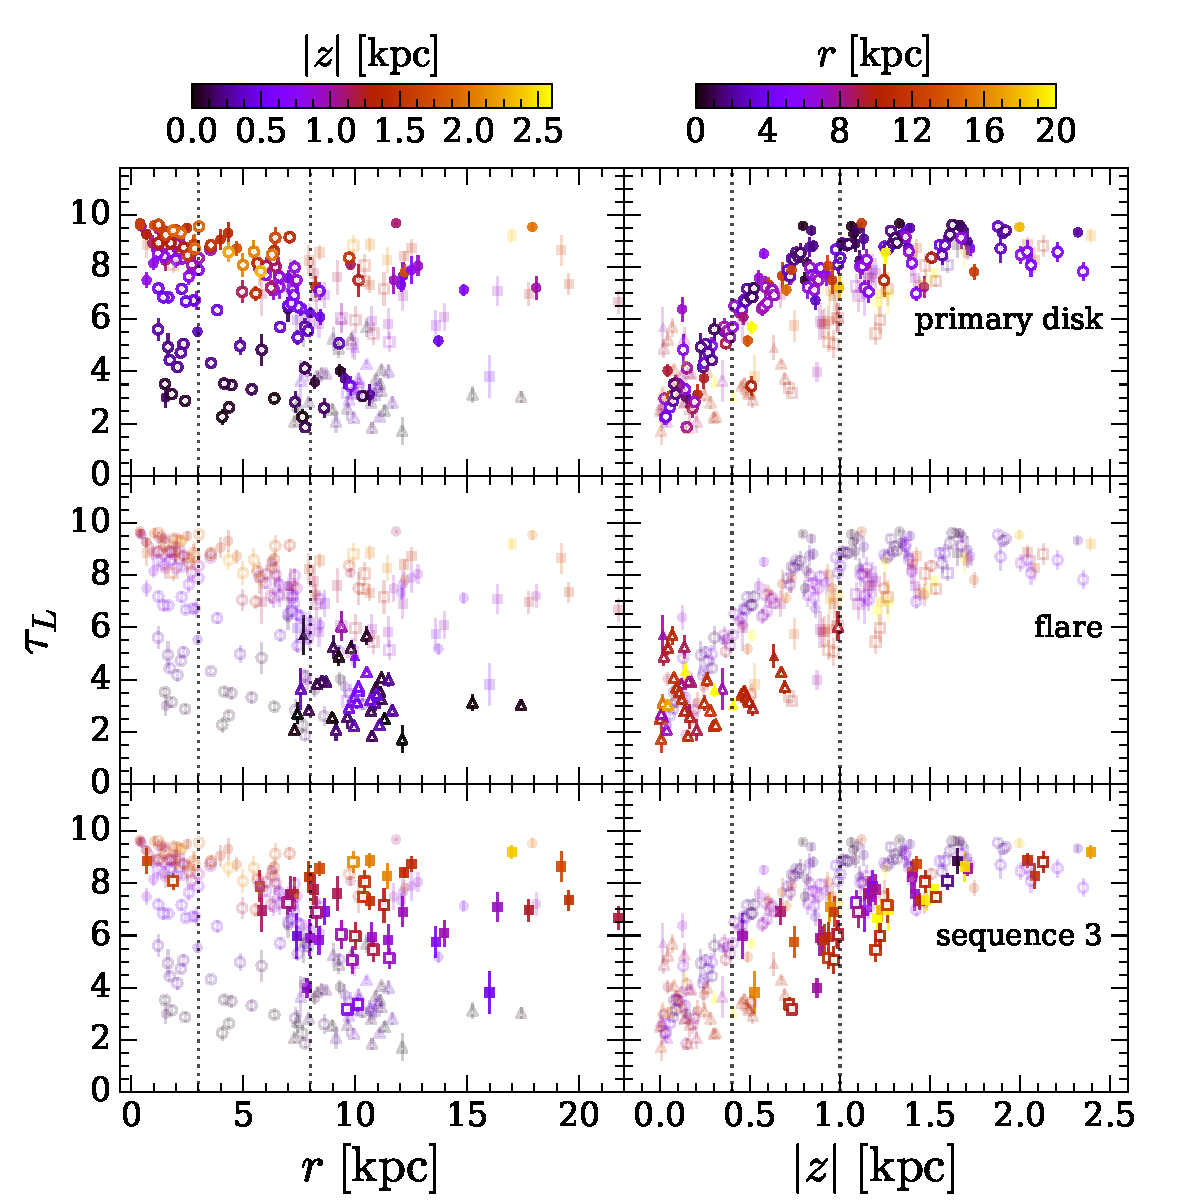
\includegraphics[width=\textwidth]{891_2/figs/MLWA_rz_all.pdf}
%%   \caption[$\tau_L$ vs
%%     ($r,|z|$)]{\fixspacing\label{891_2:fig:MLWA_rz}$\tau_L$ as a
%%     function of true radius (\emph{left}) and height
%%     (\emph{right}). On each side the points are color coded by the
%%     opposite position parameter. Open and filled circles correspond to
%%     the approaching ($r_\mathrm{proj} < 0$) and receding
%%     ($r_\mathrm{proj}\geq 0$) side of NGC 891, respectively. Vertical
%%     dotted lines correspond to the radial and vertical cuts used in
%%     \ref{chap:891_1} and Figure \ref{891_2:fig:SFH_cuts}. The three
%%     rows show the exactly the same data, but shaded to highlight the
%%     feature identified in the right-hand labels.}
%% \end{figure*}

%% Figure \ref{891_2:fig:MLWA_rz} shows the projection of our data onto the
%% $\tau_L(r,z)$ plane. The three broadly defined regions from
%% \ref{chap:891_1} are immediately obvious in the top-right
%% panel (i.e., primary disk): below \val{0.4}{kpc} all of the
%% populations are young (\val{< 6}{Gyr}), the region where $0.4 < |z|
%% \leq \val{1}{kpc}$ is a transition zone where the age generally
%% increases, and above \val{1}{kpc} the average population age
%% asymptotes to the oldest age (\val{\asim 10}{Gyr}). As described in
%% \S\ref{891_2:sec:sys_err} the specific value of $\tau_L$ at the largest
%% heights is dependent on the physical assumptions made when
%% constructing the models (i.e., the first stars in the Universe formed
%% \val{\asim 12}{Gyr} ago), but these assumptions only modulate the
%% actual value; the conclusion that the integrated light is dominated by
%% the oldest possible populations above \val{1}{kpc} is valid regardless
%% of the specific population age.

%% \citet{Xilouris99} fit a single stellar disk to broad band photometric
%% profiles of NGC 891 and find a scale height of 0.38 - \val{0.43}{kpc}
%% from $K$ to $B$ bands. In this context it is plausible that our
%% primary disk roughly corresponds to this single stellar disk. However,
%% more recent studies of NGC 891 \citep{Schechtman-Rook12,
%%   Schechtman-Rook13, Schechtman-Rook14} have refined this single-disk
%% mode to include three distinct disk components: super-thin, thin, and
%% thick with scale heights (in $K_S$ band) of 0.16, 0.47, and
%% \val{1.44}{kpc}, respectively. In this view it is likely that the
%% smooth transition from young to old ages seen in the upper-left panel
%% of Figure \ref{891_2:fig:MLWA_rz} is a result of the superposition of these
%% different disk components and thus our primary ``disk'' encapsulates
%% substructure beyond our measurement capabilities. Furthermore, the
%% primary disk also does not extend much beyond $r=\val{8}{kpc}$, which
%% is where \citet{Schechtman-Rook13} identify a truncation in their
%% super-thin disk

%% %++++++++++
%% %% {\bf MAB: Xilouris99 is a fine place to start, but I would like you to
%% %%   move on from discussing the Xilourin99 single-disk fit to the more
%% %%   sophisticated modeling from ASR (cite all 3 papers). With that in
%% %%   mind you should consider the different radial zones and how the
%% %%   flare fits in with that.

%% %++++++++++
%% %% I don't agree with your statement that above 1 kpc we are seeing the
%% %% halo as opposed to the thick disk. The points I would like to see
%% %% emphasized are that (1) there is a smooth trend of increasing age with
%% %% height that plateaus above 1 kpc. (2) At intermediate heights there is
%% %% considerable variation in age that you will then proceed to explain by
%% %% the flare and sequence-3. (3) That the 'primary disk' or sequence-1
%% %% appears to be limited primarily to the inner 8 kpc, corresponding to
%% %% the radial break of the super-thin disk seen by ASR. The thicker
%% %% component seems to be radially shorter and quite old suggesting it is
%% %% associated with the old inner disk and pseudo bulge. The thinner
%% %% portion has a range of ages. As a whole, the upper age envelop of the
%% %% 'primary disk' or sequence-1 appear to drop rapidly beyond 6 kpc.

%% %% }

%% Radial trends in $\tau_L$ reveal detailed substructure in NGC 891. The
%% top-left panel of Figure \ref{891_2:fig:MLWA_rz} confirms that, in the
%% primary disk at a given radius, older populations occupy larger
%% heights, but it is also clear that the maximum age at these large
%% heights decreases slightly with increasing radius.

%% %--------------
%% %% {\bf MAB: I agree generally with the age-radius trend except sequence-3
%% %% kind of mucks this up. Thoughts?}

%% The middle row of Figure \ref{891_2:fig:MLWA_rz} highlights the flare of NGC
%% 891. At low heights it occupies the same $\tau_L$ space as the main,
%% primary disk, but as height increases the ages stay relatively young
%% compared to the main disk. Importantly almost all of the apertures
%% belonging to this sequence exist at radii beyond \val{8}{kpc}, which
%% is one of the main reasons we identify this feature as a flared
%% extension of the star forming disk. Such a flare would be manifest as
%% an increase in scale height with radius and thus the star-forming disk
%% would extend to larger heights at large radii. Given this simplistic
%% picture, and assuming the star-forming disk extends to roughly 1 scale
%% height at all radii we can roughly estimate that at radii \val{>
%%   8}{kpc} flaring has increased the scale height by roughly a factor
%% of two (up to \val{\asim 0.8}{kpc}).

%% %% {\bf MAB: how quantitative is your scale-height estimate? This is
%% %%   nice, and if it is robust we ought to quote it in the abstract.}
%% %% ADE comment: not very robust, hence the change to ``roughly estimate''

%% The bottom row of Figure \ref{891_2:fig:MLWA_rz} shows the high-metallicity
%% ``sequence 3''. It exists only at heights above \val{0.4}{kpc} and
%% mostly beyond $r = \val{8}{kpc}$ and is made up of stellar populations
%% that are generally younger than the stars from the primary disk
%% in the same ($r,z$) locations. That said it is clear that many of the
%% apertures in sequence 3 contain a significant amount of light
%% contributed by Old population stars with the slightly lower age at large
%% heights is most likely indicative of an increased contribution from I2
%% populations.

%% %++++++++++++=
%% %% {\bf MAB: ``O population stars'' is very confusing because I read this
%% %%   as ``O stars,'' i.e., hot young stars not old DFK. So we have to be
%% %%   careful.}

%% % beyond these general trends there is evidence that at larger radii ($r
%% % > \val{\asim 8}{kpc}$) there is a separate grouping of points that
%% % occupy a younger locus than the rest of the data at similar
%% % radii. This seconday population still exhibits a general ageing of
%% % stellar population with height, but at values systematically below the
%% % main trend. Given the clumping of this younger grouping in both $r$
%% % and $z$ it is reasonable to assume that it occupies a coherent
%% % sub-structure in NGC 891. A flared disk has been suspected {\bf REF!}
%% % and would explain the presence of young stellar populations at larger
%% % heights. 

%% \subsubsection{{\Large $A_V$}}

%% \begin{figure*}
%%   \centering
%%   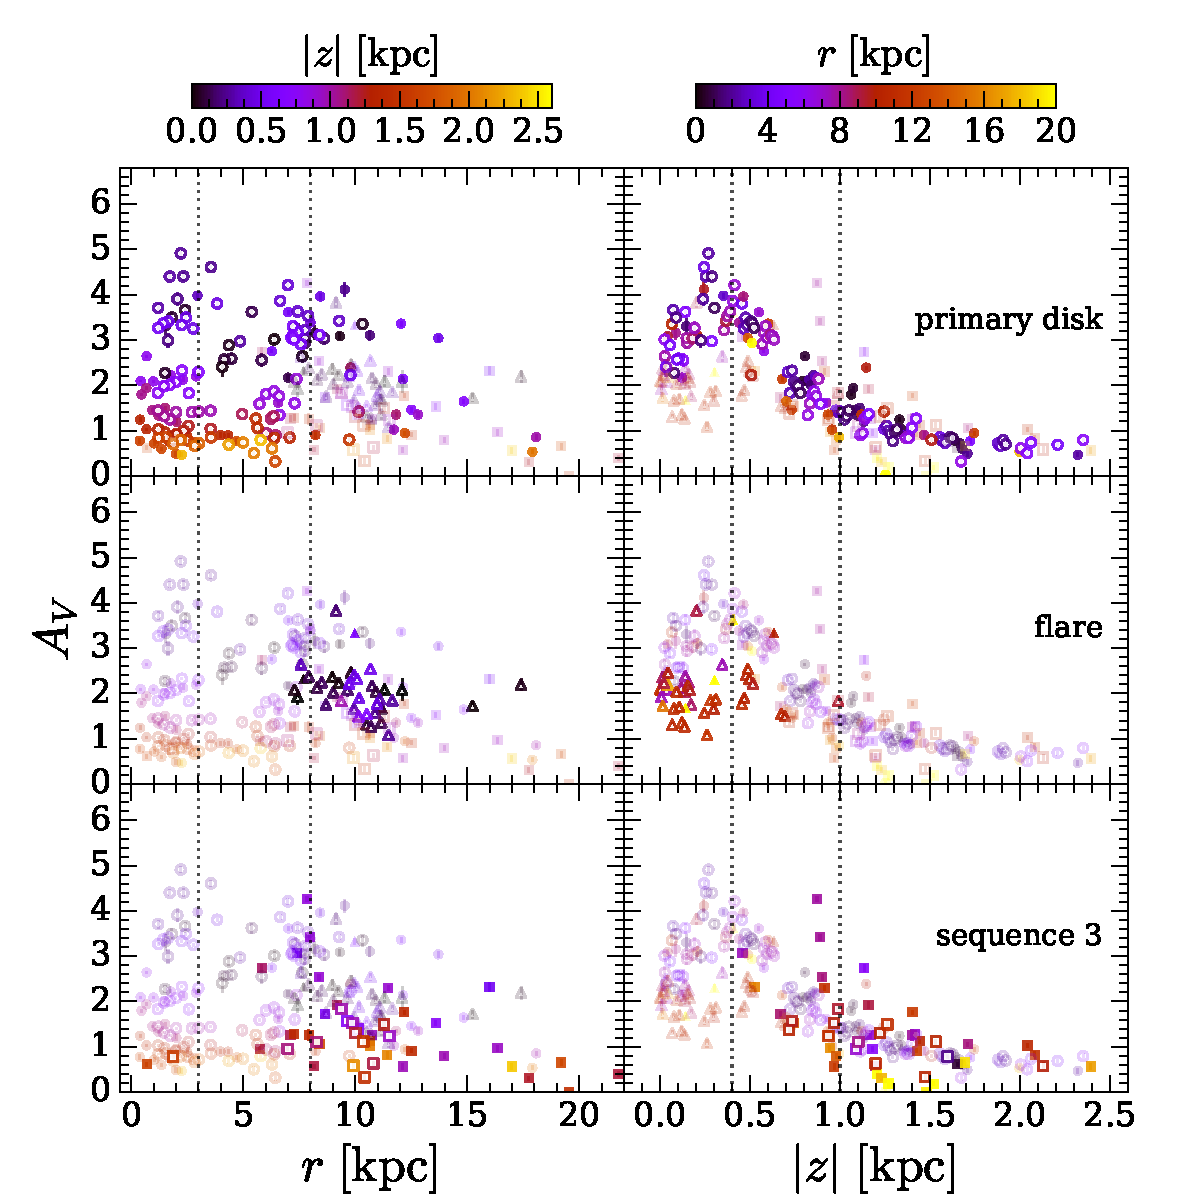
\includegraphics[width=\textwidth]{891_2/figs/AV_rz_all.pdf}
%%   \caption[$A_V$ vs ($r,|z|$)]{\fixspacing\label{891_2:fig:AV_rz}$A_V$
%%     as a function of true radius (\emph{left}) and height
%%     (\emph{right}), plotted in the same style as Figure
%%     \ref{891_2:fig:MLWA_rz}}
%% \end{figure*}

%% In Figure \ref{891_2:fig:AV_rz} the three morphological features mentioned
%% above are identified in the $A_V(r,z)$ plane. The primary disk (top
%% row) shows slightly increasing extinction with height below \val{\asim
%%   0.4}{kpc} followed by a roughly exponential decrease with height
%% above \val{\asim0.4}{kpc}. These results lend further proof to the
%% conclusion that the region below \val{0.4}{kpc} is the location of
%% current star formation, which requires regions of optically thick dust
%% and gas. Above \val{0.4}{kpc} the older stars are likely to be
%% smoothly distributed in a way that is uncorrelated with the dust. Thus
%% at the heights where old stars dominate we measure a reasonable
%% estimate of some mean extinction along a significant line of sight. At
%% low heights the dust is patchy, very dense, and correlated with
%% younger stars and so our line of sight is likely to be abruptly
%% truncated at some relatively short line of sight, and hence the stars
%% we \emph{do} see have relatively little extinction, hence the lower
%% extinction values below \val{0.4}{kpc}.

%% %----------------
%% %% {\bf MAB: Do you mean to say that $A_V(r)$ is an exponential
%% %%   function of $r$ above 0.2 kpc? Draw or fit a curve? This is the
%% %%   place to compare $A_V$ with the Balmer values. It would be
%% %%   particularly interesting to see if the different groups (primary,
%% %%   flare, seq-3) are different in this comparison. More on the
%% %%   radial trend in the next par.}
%% %% ADE: Not sure what you mean by $A_V(r)$ being exponential above 0.2 kpc.

%% %+++++++++++++++
%% %% {bf MAB: Here, concerning the down-turn at very low heights, let me
%% %%   say this differently and perhaps more plausibly. The down-turn at
%% %%   very low radii seems implausible, but we need to consider the
%% %%   transition from young to old populations seen in the previous
%% %%   figure. The older stars are likely to be smoothly distributed in a
%% %%   way that is uncorrelated with the dust. When the old stars dominate
%% %%   at larger heights we get a reasonable estimate of some mean
%% %%   extinction along a significant line of sight. At low height, since
%% %%   the dust is patchy, very dense, and correlated with younger stars,
%% %%   our line of sight is likely to be abruptly truncated at some
%% %%   relatively short line of sight, and hence the stars we do see have
%% %%   relatively little extinction. This should correspond to the LOS
%% %%   depths, which is why it would be nice to show the trend with height
%% %%   to refer back to here.

%% %% }

%% Above \val{0.4}{kpc} the general decline in $A_V$ is consistent with
%% the simple morphological view of exponentially decreasing surface
%% density in edge-on galaxies. The rate of decline shown in Figure
%% \ref{891_2:fig:AV_rz} indicates the scale height of attenuating material is
%% \val{\asim 0.6}{kpc}, which is significantly larger than either
%% \citet{Xilouris99} or \citet{Schechtman-Rook12}, who find a vertical
%% dust scale height of 0.3 and \val{0.24}{kpc} in the $V$ and $K_S$
%% bands, respectively. It is important to note, however, that both of
%% these studies find a wavelength dependence on extinction that is
%% steeper than the model of \citet{Charlot00} used in our model galaxies
%% (see \S\ref{891_2:sec:extinction}). Our prescription of extinction therefore
%% requires larger normalization values ($A_V$) to achieve the same level
%% of extinction which makes direct comparison of our data to the
%% conclusions of \citet{Xilouris99} or \citet{Schechtman-Rook12}
%% difficult.

%% %++++++++++++++
%% %% {\bf MAB: This is nice. Finish the analysis, include the results from ASR,
%% %% use all of the dust scale-heights for the different bands and let's
%% %% see if we can work this out. Show a model curve.}

%% The middle row of Figure \ref{891_2:fig:AV_rz} shows that flared extension
%% of the primary disk has systematically lower extinction than the main
%% disk. In a flared disk with a roughly constant total dust fraction an
%% increase in scale height at large radii (i.e., the flare) would cause
%% the dust surface density to decrease at these larger radii, which is
%% consistent with the lower values of $A_V$ seen in the data
%% corresponding to the flare. A paucity of data points above $z =
%% \val{0.4}{kpc}$ and within $r = \val{8}{kpc}$ makes it difficult to
%% determine vertical or radial trends in the flare's extinction, but to
%% 1st order these trends appear to be constant.

%% %--------------
%% %% {\bf MAB: My read of Figure \ref{891_2:fig:AV_rz} is that there is evidence
%% %%   for a decrease in extinction at lower heights at larger radii.}
%% %% ADE: I don't agree with this

%% Sequence 3 does not stand out very much in the $A_V(r,z)$ planes. It
%% shows extinction values that are generally consistent with the other
%% morphological features that exist at smaller radii, albeit with more
%% scatter (bottom right panel of Figure \ref{891_2:fig:AV_rz}).

%% %++++++++++++++++++
%% %% {\bf MAB: My read of Figure \ref{891_2:fig:AV_rz} is that it is hard to
%% %%   conclude on seq-3 except to see that it appears to have much more
%% %%   variation in $A_V$ with height, although it does not appear to be
%% %%   inconsistent at a given height with its counterpart populations at
%% %%   smaller radius. I think you say much of this and I don't think it is
%% %%   important to emphasize that seq-3 ``occupies a locus with lower
%% %%   extinction than either the star forming disk or the flare'' because
%% %%   I think this can be explained by height.}

%% \subsubsection{{\Large $Z_L$}}

%% \begin{figure*}
%%   \centering
%%   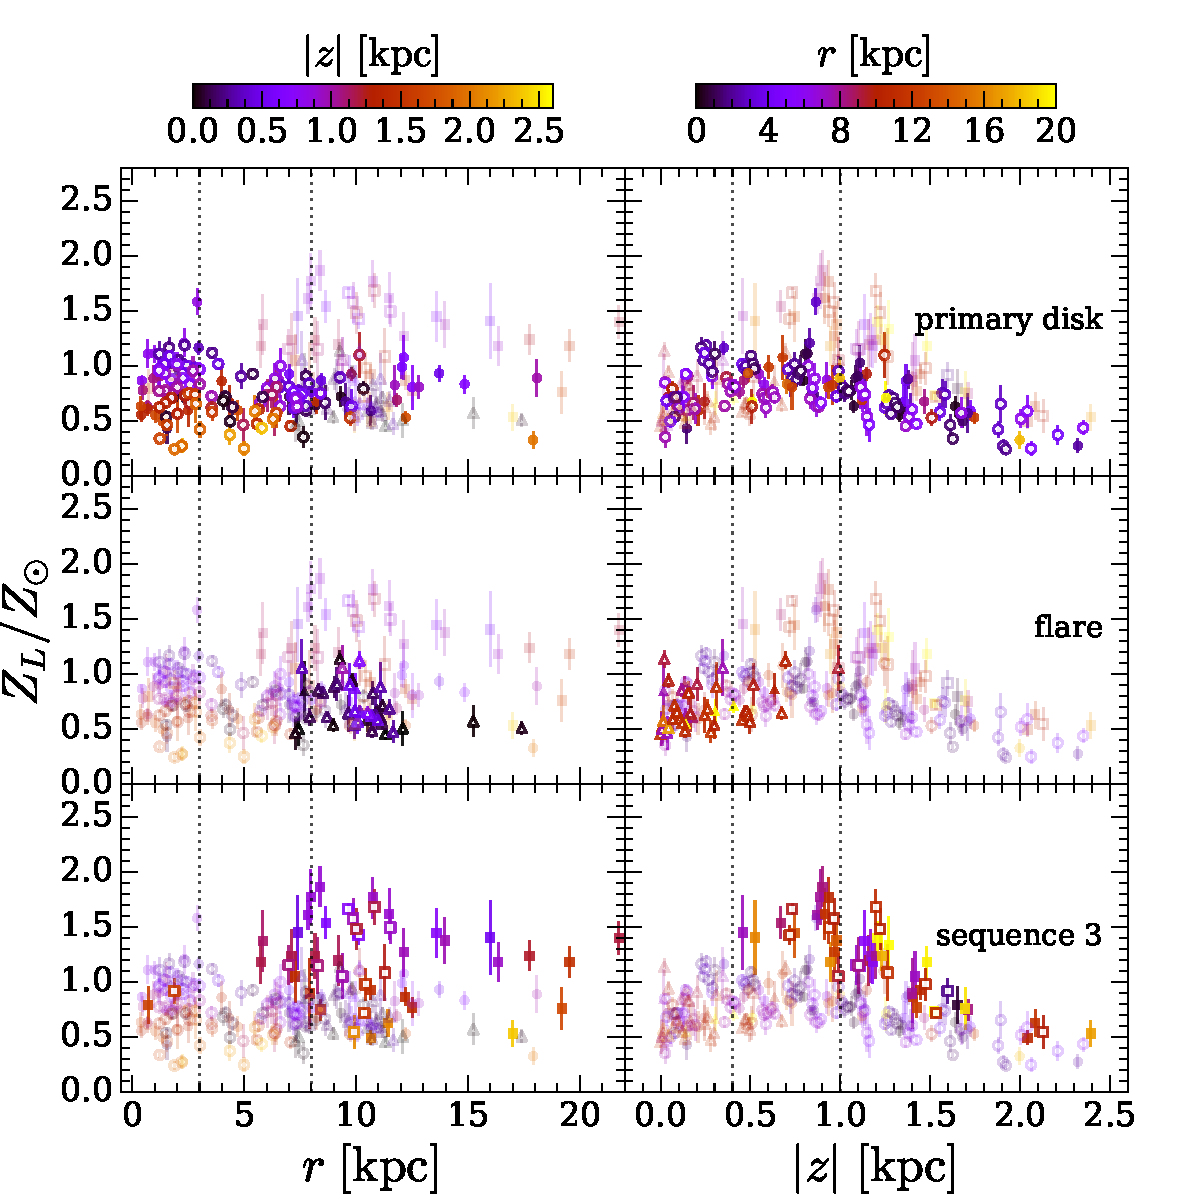
\includegraphics[width=\textwidth]{891_2/figs/MLWZ_rz_all.pdf}
%%   \caption[$Z_L$ vs
%%     ($r,|z|$)]{\fixspacing\label{891_2:fig:MLWZ_rz}$Z_L$ as a function
%%     of true radius (\emph{left}) and height (\emph{right}), plotted in
%%     the same style as Figure \ref{891_2:fig:MLWA_rz}}
%% \end{figure*}

%% Finally, Figure \ref{891_2:fig:MLWZ_rz} shows $Z_L$ as a function of
%% location in NGC 891 and highlights the discriminatory power of
%% metallicity in identifying the three morphological features mentioned
%% above. The primary disk shows slightly negative correlations
%% between metallicity and both radius and height (top panel). This view
%% is consistent with measurements from the Milky Way \citep{Bovy12,
%%   Hayden14} and with the conclusions of
%% \ref{chap:891_1}. This also reaffirms the idea that stars at
%% large heights are formed from pristine gas at early times (as shown in
%% Figure \ref{891_2:fig:MLWA_rz}.

%% In the middle row of Figure \ref{891_2:fig:MLWZ_rz} shows strong evidence
%% that the flare identified in previous sections comes from the same
%% underlying distribution as the primary disk. At all radii and heights
%% in the $Z_L(r,z)$ plane the flare points are essentially
%% indistinguishable from those of the primary disk. The flare exists in
%% a different ($r,z,A_V$) location, but it's ages and, importantly,
%% metallicity are consistent with the same populations seen in the disk.

%% %% {\bf MAB: don't push too hard on Z for young-age pops.}  

%% Sequence 3 is perhaps most visible as a high-metallicity sequence in
%% the $Z_L(r,z)$ planes, as shown in the bottom row of Figure
%% \ref{891_2:fig:MLWZ_rz}. At all radii and heights it occupies a locus that
%% has larger values of $Z_L$ than either the primary disk or the flare
%% (which are the same in terms of metallicity). Despite these high
%% values it still follows a general trend of decreasing metallicity with
%% height and radius, which suggest that whatever evolutionary mechanisms
%% cause the trends in the disk also affect the large radii and heights
%% occupied by sequence 3.

%% %% These results, coupled with those shown in Figure \ref{891_2:fig:MLWA_rz}
%% %% yield a possible explanation for the presence of sequence 3. This
%% %% sequence is distinct in both age and metallicity from the primary disk
%% %% and flare

%% %+++++++++++++++
%% %% {\bf MAB: Isn't $Z_L(r,z)$ a volume not a plane? Maybe another way to
%% %%   say your last point which also ties in to the flare is that we are
%% %%   seeing a population sequence at large radii and large heights that
%% %%   is distinct in both age and metallicity from what looks to be the
%% %%   old thick disk seen over a range of radii. It may be a temporal
%% %%   extension of the flare seen at younger ages, i.e., stars that formed
%% %%   in a flared disk at an intermediate era.}

%% %% ADE: This is nice, but how does the temporal fare extension picture
%% %% jive with \emph{higher} metallicities than the younger flare?

%% % The average metallicity appears to increase slightly with
%% % height up to \val{1}{kpc} where it abruptly begins to decrease with
%% % increasing height. We note, however, that the apparant increase up to
%% % \val{1}{kpc} is driven mostly by a few super-solar points between 0.4
%% % and \val{1}{kpc} and at large radii. As we have seen above, the radial
%% % structure of NGC 891 is highly non-uniform and we therefore caution
%% % that these few points are probably not representative of a global
%% % trend. Thus ignoring these super-solar points the average metallicity
%% % is relatively constant below \val{1}{kpc}, at which point it decreases
%% % with height. This general trend is qualitatively consistent with
%% % results from the Solar cylinder in the Milky Way
%% % \citep{Hayden15,Bovy12} and supports the theory that large heights are
%% % primarily populated by old stars that formed from pristine gas.

%% % Much like $\tau_L$ and $A_V$ there appears to be a second order,
%% % bi-modal $Z_L$ distribution in NGC 891. Starting at $z = \val{\asim
%% %   0.4}{kpc}$ there is a cluster of apertures with super-solar
%% % metallicities that follow the same general trend as the global average
%% % (i.e., decreasing with radius above \val{1}{kpc}), but at a higher
%% % metallicity. All of these high-$Z_L$ apertures exist at radii beyond
%% % \val{8}{kpc}, which suggests they belong to the same sub-structure
%% % identified in $\tau_L$. Under the assumption that this sub-structure
%% % is a flared disk the presence of high metallicity stellar populations
%% % indicate that this disk is likely the site of a recent epoch of star
%% % formation, a claim supported by the systematically lower ages see in
%% % Figure \ref{891_2:fig:MLWA_rz} for the same structure.

\subsection{Star Formation History}
\label{891_2:sec:SFH}
\begin{figure*}
  \centering
  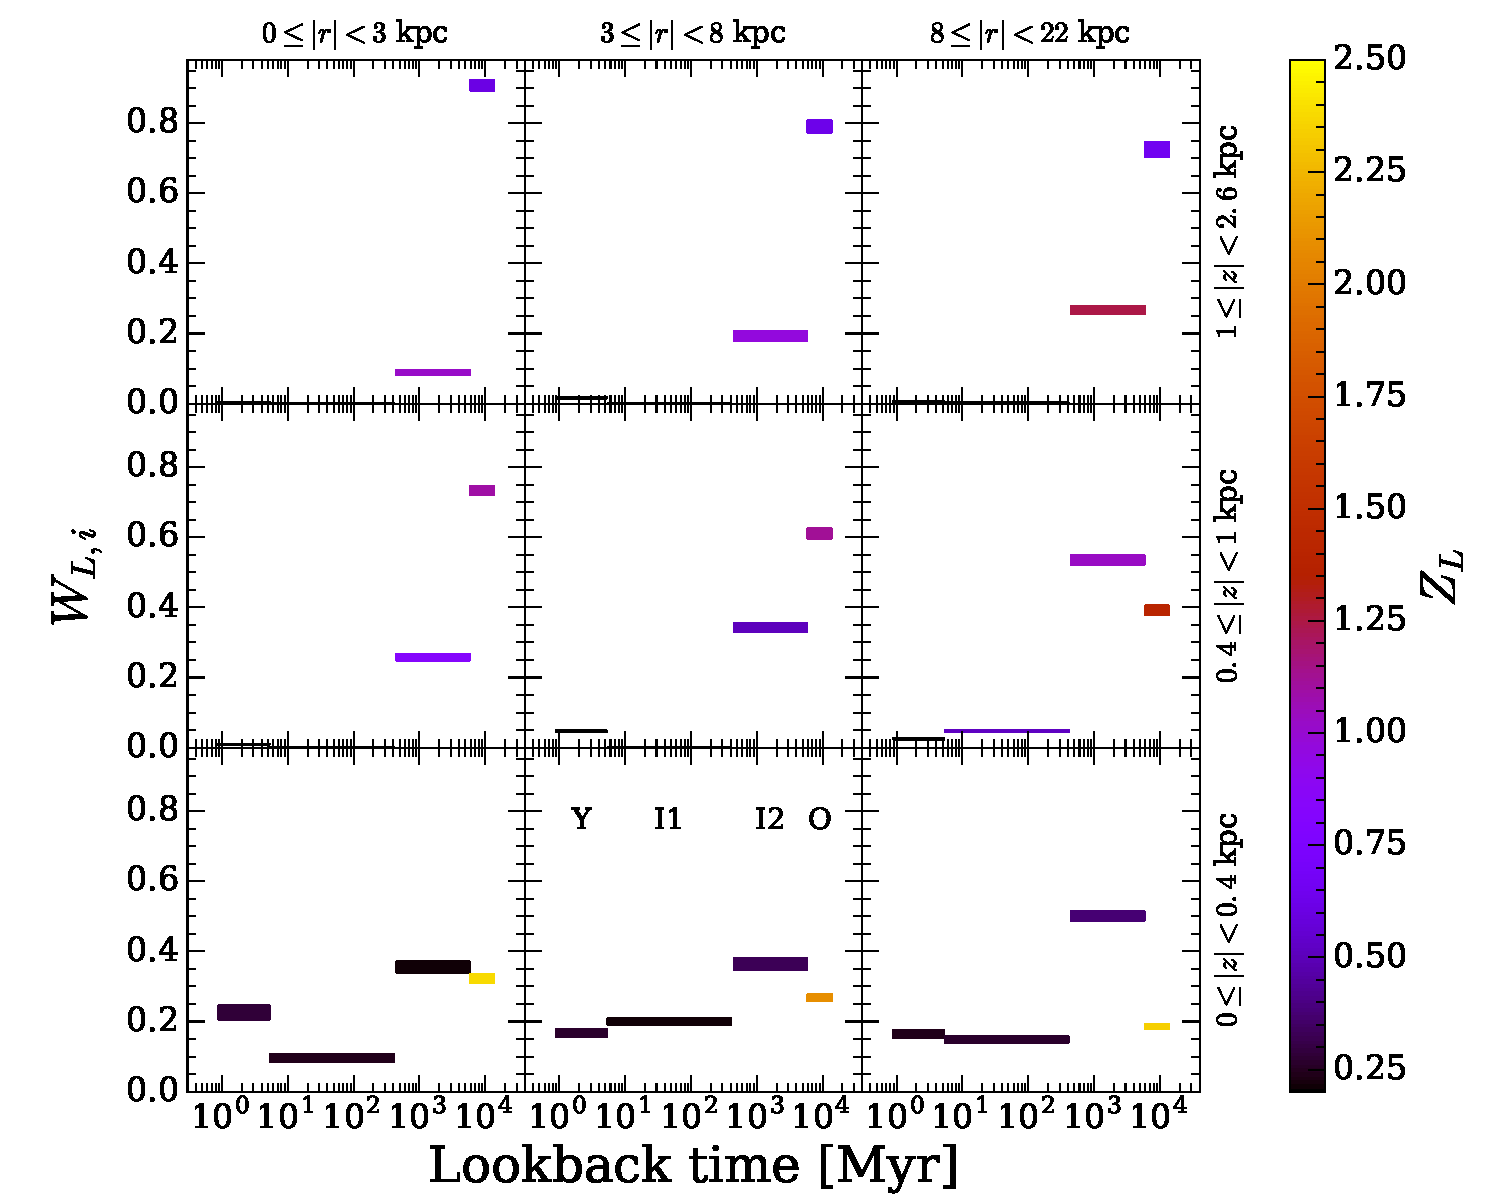
\includegraphics[width=\textwidth]{891_2/figs/SFH_cuts.pdf}
  \caption[SSP light weights in ($r,|z|$)
    grid]{\fixspacing\label{891_2:fig:SFH_cuts}Fractional light-weight
    (Equation \ref{891_2:eq:light_weight}) for each DFK age bin as a
    function of radius and height. The radial and height bins shown
    are the same as used in \ref{chap:891_1} and highlight the
    different components of NGC 891 described in the text. The
    horizontal extent of each bar spans the range of ages covered by
    each SSP and the vertical width of each bar corresponds to the
    fitting uncertainty of each weight computed using the same method
    detailed in \S\ref{891_2:sec:fit_err}. Each weight is color coded
    by the average $Z_L$ in the particular ($r,z$) bin.  }

\end{figure*}

A primary benefit of full-spectrum SSP fitting is that it allows us to
fit and measure the star formation history (SFH) for every aperture in
our data set. As discussed in \S\ref{891_2:sec:sys_err} the mean,
light-weighted age ($\tau_L$) is a convenient proxy for SFH, but
requires an assumed SFH for the models used to fit our galaxy data. To
avoid these assumptions we can examine the integral of the SFH
multiplied by the flux of each SSP, which is identical to the
light-weights found during SSP fitting (see
\S\ref{891_2:sec:SSP_method} and Equation \ref{891_2:eq:MLWA}). Figure
\ref{891_2:fig:SFH_cuts} shows these values in the same grid of radius
and height used in \ref{chap:891_1} (although now the radius values
are the true, cylindrical values a la \S\ref{891_2:sec:LOS}). From
these data we can see the same general trend found in \ref{chap:891_1}
and above: younger populations predominantly exist below
\val{0.4}{kpc}. There are also small contributions from young
populations above \val{0.4}{kpc} at the largest radii, which confirms
the idea that NGC 891 built up from a superposition of flared disks
with increasing ``flare radii''.

Above \val{0.4}{kpc} (and even below this for $r < \val{8}{kpc}$) the
I2 populations contribute more to the total light at larger radii,
with a corresponding decrease in the contribution from Old
populations. This trend is broadly consistent with an inside-out view
of star formation in NGC 891. Such a formation scenario (which we also
see in \ref{chap:891_1}) predicts a higher fraction of young and
intermediate aged stars at large radii, exactly as seen in Figure
\ref{891_2:fig:SFH_cuts}.

%% Further evidence for a flare can be seen in the fact that I2
%% populations (see Table \ref{891_2:tab:dfk}) contribute more to the total
%% light at larger radii, with a corresponding decrease in contribution
%% from O populations. This picture provides further insight into
%% secondary morphological feature (i.e., flare) identified in
%% \S\ref{891_2:sec:rz}, specifically that, while it shows the same positive
%% age/height gradient seen in the main primary disk, its oldest
%% stellar populations are at most \val{\asim5.7}{Gyr} old (i.e., the old
%% limit of the I2 DFK bin). 

%% {\bf MAB: I am not sure I followed this paragraph. It is not clear to
%% me that the trends in O and I2 DFKs in the 6 bins for $z>0.4$ kpc
%% are consistent with flares. What if the thick disk is simply
%% younger at larger radii. Maybe I am missing something?}

%% Despite this decrease O populations are still the primary source of
%% light for all radii at heights above \val{1}{kpc}. This observation is
%% consistent with the conclusions from \S\ref{891_2:sec:rz} that any flare in
%% NGC 891 extends up to \val{\asim 1}{kpc}, but not much beyond this
%% height.

%++++++++++++++++++++++
%% {\bf MAB: In this discussion I think we need to be careful what we
%%   mean by flare. For example, the Martig+14 simulations have all of
%%   the mono-age populations flaring, just at different radii, inside
%%   out. So when we say flare, do we mean only the Y and I1 pops?}

%% ADE: Agree, the increase in I2 with radii can more simply be
%% explained as inside out formation, which is consistant with paper1

Finally, the metallicity color-coding in Figure
\ref{891_2:fig:SFH_cuts} is consistent with the enrichment history
presented in \S\ref{891_2:sec:tZ}. The youngest populations (which
only contribute appreciable light at low heights) are very metal poor
because they are formed from pristine material that has recently
fallen onto the disk of NGC 891 (see also Figure
\ref{891_2:fig:MLWZ_rz_cut}). At these low heights the most metal-rich
population is the Old population, and indeed it is this population
that has the largest value of $Z_L$ anywhere in NGC 891. This suggests
that the Old populations at low heights correspond to the youngest
limit of the Old DFK age bin, which is exactly the age of ``peak
metallicity'' discovered in \S\ref{891_2:sec:tZ} (\val{\asim 6}{Gyr}).

We also see that the metallicity of the Old population decreases with
height (at all radii) while the metallicity of the younger populations
increases with height. Once again, this beautifully illustrates the
enrichment history presented above; the Old population formed during
the ``closed-box'' period in NGC 891's history, where older stars
(i.e., stars at larger heights) formed from pristine gas. Star
formation more recent that \val{6.6}{Gyr} (i.e., anything besides the
Old population), however, occurred during a time when metal-poor gas
from outside of NGC 891 caused \emph{younger} stars (i.e., those at
lower heights) to have decreased values of metallicity.

%% At first glance the $Z_L$ values shown in Figure
%% \ref{891_2:fig:SFH_cuts} seem counterintuitive; at the lowest heights
%% the largest values of metallicity occur in the oldest SSPs and the I2
%% SSPs show metallicity values that increase with height. The first
%% trend is likely due to the positive correlation between age and
%% metallicity identified at low heights in
%% \S\ref{891_2:sec:fit_err}. Indeed, below \val{0.4}{kpc} the Y and I1
%% SSPs are very metal poor, while I2 and O have higher metallicities,
%% consistent with the degeneracies seen at these low heights. In other
%% words, the high metallicity in Old populations below \val{0.4}{kpc} is
%% likely a result of fitting degeneracies and perhaps not an accurate
%% representation of the physical picture in these regions.

%% %++++++++++++
%% %% {\bf MAB: This hi-Z O population at low heights has me concerned.  Do
%% %%   we think this is real or an artifact of our fitting?  It could be
%% %%   real if there is indeed an old, metal-rich thin disk, although one
%% %%   wonders why I2 is so metal poor at the same height. Since we have
%% %%   supposedly corrected for projection and have everything in the right
%% %%   radial bins it would be hard to invoke the older stars being from
%% %%   smaller radii where metallicity is higher. So this is why I wanted
%% %%   to see mass-weighted plots.}

%% To explain the trend in increasing metallicity with height seen in the
%% I2 populations we invoke the flare identified in this and previous
%% sections. Recent star formation in the ``normal'' primary disk (i.e.,
%% not the flare) does not extend much above \val{\asim 1}{kpc} and any
%% stars at these large heights are likely to be old and metal poor. The
%% flare, on the other hand, as shown above, exhibits recent (in this
%% case \val{\asim 6}{Gyr} ago) star formation at heights above
%% \val{1}{kpc}. Thus, as height increases the fraction of I2 stars that
%% belong to the flare (and therefore have higher metallicities)
%% increases and the average $Z_L$ in the I2 bin increases. This
%% interpretation is consistent with the morphological picture present in
%% \S\ref{891_2:sec:rz} and allows us to actually infer something about the SFH
%% in NGC 891. As shown in Table \ref{891_2:tab:dfk} the I2 bin spans roughly
%% \val{5}{Gyr} which is a significant fraction of the total age of NGC
%% 891 (assumed here to be \val{12}{Gyr}). In the primary disk I2 stars
%% are considered ``old'', have low metallicities, and were therefore
%% likely formed at the older end of the I2 bin (\val{\asim 6}{Gyr}). At
%% larger heights, however, light from the flare dominates in all but the
%% oldest SSP bin, and thus the I2 DFK bin represents a fundamentally
%% different population of stars; those that formed near the young limit
%% of the I2 bin (i.e., \val{\asim 500}{Myr}) and therefore have higher
%% metallicities (as seen in Figure \ref{891_2:fig:SFH_cuts}).

%----------------
%% {\bf MAB: I don't understand the first sentence. Do you mean the
%%   positive metallicity gradient with radius for I2 at each height? Or
%%   do you mean the positive gradient in WL with radius for all heights?
%%   Or ...?  I would drop the claim that stars above 1 kpc are
%%   ``primordial halo stars that are coeval with NGC 891.'' You just
%%   don't know that. If you want to assume it, and then see what follows
%%   that's a different matter. In any evet I would not assume they are
%%   part of the halo.

%% I'm not sure I buy this and what follows: ``Thus, as height increases
%% the fraction of I2 stars that belong to the flare (and therefore have
%% higher metallicities) increases and the average $Z_L$ in the I2 bin
%% increases.'' Again, why is this all due to the flare as opposed to an
%% outer thick disk what has different age and metallicity properties
%% because of some inside-out formation?

%% ADE: I see what you're saying about ``why flare and not just a thicker
%% disk'', but I really think that Figure \ref{891_2:fig:MLWA_rz} tips the
%% scales in favor of a flare. Basically, the fact that our ``flare''
%% only exists at large radii rules out a thicker disk. Right? 
%% }


%% Given the data shown in Figure \ref{891_2:fig:MLWA_rz} we conclude that the
%% majority of the flare stars are coveal with the main star forming
%% disk, which suggests the flare is simply an increase in scale height
%% (of both gas and stars) at larger radii and not representative of a
%% fundamentally different population. Figure \ref{891_2:fig:MLWZ_rz}, however,
%% suggests that the flare stars \emph{do} occupy a location in parameter
%% space separate from the primary disk; one of higher
%% metallicity. The true picture is likely somewhere in the middle;
%% what's certain is that stars in the ``flare'' have a similar SFH as
%% the main primary disk but formed from gas with a higher
%% metallicity than that found towards the inner regions of NGC 891.

%++++++++++++++++++
%% {\bf MAB: We should talk about this. I don't have my head wrapped
%%   around it so I am not yet onboard.}

%% ADE: Ya, I don't get it either. Not sure what I was thinking
%% here. Figure 21 clearly shows that the ``flare'' stars have the
%% same metallicity as the primary disk. Just took it out for now.

%% The first order effect that we are seeing is that there is a positive
%% age gradient with height above the mid-plane, consistent with
%% qualitative expectations.

%% Lower metallicity (sub-solar) models appear to give flatter age
%% profiles at large height, which is what we would expect.  In contrast,
%% models with solar and above metallicity yield lower ages at the
%% largest heights relative to mid-latitude values, i.e., the ages roll
%% over a bit at large heights.  This may very well be a systematic
%% effect if indeed the high-latitude population is intrinsically
%% low-metallicity since forcing higher metallicity increases
%% line-strength which would then have to be compensated for in the model
%% fitting with younger ages. On the other hand, we need to be careful
%% (a) not to over-interpret small changes in age at large ages (where
%% there is little leverage in the models; and (b) not to make
%% conclusions based on our initial assumptions.

%% We don't see much correlation of the optical depth with the adopted
%% metallicity of the SPS models. We should quantify this, but it is
%% reassuring. This means, for example, that metallicity and age are
%% largely keying off the line-strengths and not the continuum spectral
%% shape, but we should check this in detail--for example, by looking at
%% correlations between age vs $A_V$ in residuals about the mean at a
%% given height.

%% There do appear to be radial trends in the sense that the outer disk
%% is younger, and younger at a given height, although this trend has not
%% been isolated from metallicity effects (e.g., perhaps the outer disk
%% is also more metal poor, as seen in the Milky Way).

%% We also have not looked carefully to determine if the age gradients
%% are symmetric with radius on either side of the galaxy.


\section{Summary}
\label{891_2:sec:summary}

We have used full-spectrum SSP fitting measure trends in $\tau_L$,
$Z_L$, and $A_V$ with both radius and height in NGC 891. To mitigate
the impact of degeneracies between these quantities we downselect the
full \citetalias{Bruzual03} SSP template library in two ways: limiting
the range of metallicity values used, and reducing the age resolution
of the template library. We limit the range of allowed metallicities
to be $Z \geq 0.2\Zsol$ and show in \S\ref{891_2:sec:multi_metal} that SSPs
with lower metallicity produce model galaxies that; a) are
statistically worse than higher metallicities, in a $\chi^2$ sense, and
b) result in the astrophysically implausible situation of very old
super-solar metallicity stars combined with very young super metal
poor stars.

The age resolution of our SSP template libraries is reduced using the
statistically motivated method of diffusion K-means
\citepalias{Mosby15}, which accounts for the fact that there is very
little difference in spectral shape between old SSPs over a range of
roughly \val{5}{Gyr}. We find that this limited basis set still
accurately reproduces our observed galaxy spectra
(\S\ref{891_2:sec:final_SSP}).

While these steps do reduce the magnitude of degeneracies between
$\tau_L$, $Z_L$, and $A_V$ these degeneracies are still the dominant
sources of uncertainty in our fit parameters. However the are
typically on the order of \asim 10\%, which still allows us to measure
trends in radius and height. We also find two distinct regimes of
degeneracy between $\tau_L$ and $Z_L$; for intermediate and old
populations these two quantities are negatively correlated (as
expected from e.g., \citet{Oconnel76,Aaronson78,Worthey94,dePaz02})
but for young populations $\tau_L$ and $Z_L$ are positively
correlated, indicating that older populations have higher
metallicities. This correlation is caused by the interplay between all
three of our fit parameters, as discussed in \S\ref{891_2:sec:fit_err},
underlining the importance of parameter covariance in understanding
fit uncertainties.

%++++++++++++++++++++
%% {\bf MAB: In the above two paragraphs I think you want to say a bit
%%   more about the motivation behind reducing the number of templates
%% in the context of degeneracies and systematic errors.

%% Specifically, you have reduced the {\it range} of metallicity, and you
%% have reduced the {\it resolution} in age. You should say that both are
%% important, that you should specify that you have done both, and give
%% what that reduction is (metallicities cut; reduction to 4 age bins
%% with characteristic ages of [t1,...t4] Gyr via DFK). Then you should
%% say that limiting the metallicity range is crucial because of fitting
%% degeneracies that lead to astrophysically implausible stellar mixes of
%% very young and ultra metal-poor stars mixed with very old and super
%% metal-rich stars. Reducing the age resolution is particularly
%% important at older ages where there is little to no leverage from the
%% full spectral fitting to discriminate between 5 Gyr. These reductions
%% allow you to minimize and quantify the degeneracies between age and
%% metallicity and quantify the systematic uncertainties in the mean age,
%% as you will describe in the next paragraph.

%% I would not refer to the two degeneracy regimes by the physical
%% location in the galaxy, but by the characteristic age of the stellar
%% populations (see the request to do this earlier in the relevant
%% section). This is more fundamental and allows other studies to use the
%% information directly. You then can mention that these characteristic
%% age regimes happen to correspond to height regimes for NGC 891 given
%% its edge-on orientation.

%% }

While we use $\tau_L$ as a proxy for star formation history we caution
that any single metric of age (including $\tau_L$) requires
assumptions about the underlying star formation that will introduce
systematic offsets into the results. We quantify the magnitude of this
systematic uncertainty and find it to be, in a worst case scenario,
\asim 20\%. It is important to note, however, than for studies of a
single galaxy a worst-case scenario (which assigns a completely random
star formation history to each location in the galaxy) is a large
overestimation. On time scales greater than one dynamical time we
expect the the galaxy to be relatively well mixed which causes the
average SFH to be relatively constant and thus the systematic
uncertainties discussion in \S\ref{891_2:sec:sys_err} will not apply. At
large radii the dynamical timescale of NGC 891 is roughly 1 Gyr, which
means the systematic uncertainties in the I2 and O DFK bins are
greatly mitigated by mixing of stars within the galaxy.

%---------------
%% {\bf MAB: Again, you should note that the DFK parameterization gives a
%%   well defined framework for definning the age systematics that
%%   decouples the age-metallicity fitting degeneracies with the
%%   uncertainties inherent in age estimates from measurements of the
%%   integrated light of stellar populations (i.e., we don't measure
%%   individual stars so there is a limit to the available information in
%%   the spectra).

%% I know what you are getting at in the discussion of dynamical times
%% and mixing lengths because we talked about it, but we need to work a
%% bit more on our thinking and exposition. First, I am thinking that the
%% dynamical time, for a disk, works to sort out azimuthal variations,
%% i.e., azimuthal variations will tend to average out for stellar
%% populations older than that time-scale. I think we mean {\it radial}
%% mixing length, and this is the part that in my mind is fuzzy -- and
%% not just because of us. I don't think it is clear how much disks mix
%% radially, and if they do, how much the mixing depends on
%% height. Carlos and Elena claim that radial migration is most effective
%% for dynamically cold stars (small velocity dispersions and near the
%% mid-plane), so it is not clear how these migrating stars contribute to
%% the thicker disk component since nobody knows how to make a thick disk
%% without mergers or early-era turbulence (thick gas disk).

%% I think you are right that the 20\% systematic is an over-estimate,
%% but there could well be systematic trends in the SFH with radius and
%% height, and I don't think we can say more than that 20\% is an upper
%% limit and it is unlikely to apply at even the extrema in R and z in
%% any given galaxy.

%% }

%% ADE: Isn't that what I said? (I took out the mixing length
%% sentence, maybe this is a thought for another day).

The light weights shown in Figure \ref{891_2:fig:SFH_cuts} suggest an even
more optimistic picture, in which the SFH is relatively constant
across all of NGC 891. While the specific weights do change with $r$
and $z$, the general trends for each DFK bin are the same at all radii
and heights. For example, the strength of the I2 population increases
with radius at all heights and the strength of the O population
decreases with radius at all heights. It is more difficult to make
similar statements about the Y and I1 stellar populations because they
exist only at a narrow range of height and radius, but these
populations make up a negligible contribution to the total systematic
uncertainty. In other words the qualitative similarity in the light
weights (a proxy for the SFH) seen in Figure \ref{891_2:fig:SFH_cuts}
indicates that the underlying star formation rate does not vary
\emph{in shape} by large amounts across large regions of NGC 891, thus
uncertainties that arise from assuming a star formation history (i.e.,
\S\ref{891_2:sec:sys_err}) only effect systematics on a galactic scale;
within NGC 891 these systematics contribute negligibly to the total
uncertainty.

%---------------
%% {\bf MAB: This is important: I need to see the SFR as requested for
%%   alternative versions of Figure \ref{891_2:fig:SFH_cuts}, i.e., once with
%%   mass-weights and then one with mass-weights divided by the time
%%   interval (SFR). That said (and with these in hand), I think you
%%   might have a good argument to make. Actually I think the point that
%%   is likely robust is not that the SFH is relatively constant with R
%%   and z, but that it changes smoothly at least in R. The SFR at recent
%%   times is quite different at different heights, particularly at $R<8$
%%   kpc. However, Y and I1 are not an issue for age systematics since
%%   these are dominated by the larger time bins of I2 and O.

%% Noted you have an incomplete sentence.}

Our 3-dimensional view of NGC 891 is enhanced by deprojecting the
observed, projected radii to cylindrical radii based on kinematic
measurements of stellar populations. Thus armed with fully 3D
information about the location of our stellar populations we examine
their distribution in ($r,|z|,\tau_L,Z_L,A_V$) space and find:

%+++++++++++++++
%% {\bf MAB: don't use ``true'' because there are uncertainties. You should
%% work these out (see earlier request) and summarize here.}

\begin{enumerate}

\item Confirmation of the results from Chapter
  \ref{chap:891_1}. Namely Young populations exist only below
  \val{0.4}{kpc}, age increases from 0.4 - \val{1}{kpc}, and saturates
  above \val{1}{kpc}.

\item The picture of inside-out galaxy formation seen in Chapter
  \ref{chap:891_1} is enhanced by the view that each generation of
  stars forms a flared disk, with later generations forming disks with
  larger radii. This view is similar to the prediction of
  \citet{Martig14a}; the galaxy disk is a superposition of flared
  disks that formed with increasing radii.

\item Two distinct epochs in the enrichment history of NGC 891. During
  the first few Gyr of its life NGC 891 existed in more of a
  closed-box state; from an initial seed of pristine gas each
  generation of stars formed from gas enriched by the generations
  before it at roughly a rate of \val{0.15}{\Zsol/Gyr}. However, about
  \val{6}{Gyr} ago new, metal-poor gas from outside the galaxy started
  to fall onto the disk of NGC 891. This new gas lowered the
  metallicity of stars formed in the last \val{6}{Gyr} and the
  indication is that metallicity will continue to decrease in the
  future. This rate of decrease is about \val{-0.18}{\Zsol/Gyr}.

\item Three groupings of stellar populations in the
  ($r,|z|,\tau_L,Z_L,A_V$) parameter space: a primary disk, a flared
  extension of the disk, and a metal-rich sequence at large radii and
  heights. These groupings are \emph{not} distinct features in NGC
  891. Instead they are the consequence of the formation and
  enrichment history present above. The primary disk is the main disk
  of the galaxy and is composed of multiple mono-age, flared disks
  that increase in radius with galactic age. The ``flare'' at large
  radii is corresponds to the most recent batch of star formation. The
  third sequence is the portion of the disk that formed during peak
  metallicity, \val{\asim 6}{Gyr} ago.

\end{enumerate}

%% \begin{enumerate}
  
%% \item A ``primary'' disk that exists at all heights (at least to
%%   \val{2.6}{kpc}) and radii less than \val{8}{kpc}. In this disk there
%%   is clear evidence for the presence of young stellar populations ($<
%%   \val{\asim 400}{Myr}$ ago) below \val{0.4}{kpc} and a lack of the
%%   same populations above \val{0.4}{kpc}, consistent with the results
%%   of \ref{chap:891_1}. Above this transition emission from
%%   the disk is dominated by I2 and O stars and the average population
%%   age increases with height. This disk also exhibits negative
%%   metallicity gradients with both radius and heights, which is
%%   consistent with observations of the Milky Way. It is likely that the
%%   primary ``disk'' is actually a superposition of multiple disk
%%   components like the ones found in \citet{Schechtman-Rook13,
%%     Schechtman-Rook14}.

%% \item A flared extension of the the primary disk at radii beyond
%%   \val{8}{kpc}. This flare has the same age and metallicity properties
%%   as the main disk, but with a scale height roughly twice that of the
%%   main disk (\val{\asim 0.9}{kpc}, compared to a V-band scale height
%%   measure at small radii by \citet{Xilouris99} of
%%   \val{0.4}{kpc}). This increase in scale height decreases the total
%%   surface density of dust at large radii and the extinction is
%%   correspondingly lower, especially near the midplane.
  
%% \item A sequence of intermediate-age, super-solar metallicity
%%   populations at large heights ($|z|> \val{\asim 0.9}{kpc}$) and radii
%%   ($r>\val{8}{kpc}$). Despite their old ages, the populations in this
%%   ``third sequence'' appear to come from a fundamentally different
%%   underlying distribution from stars at similar heights but smaller
%%   radii; within $r=\val{8}{kpc}$ light at large heights is dominated
%%   by the oldest stellar populations, but in the third sequence these
%%   heights are have strong contributions from intermediate-aged
%%   populations. Despite an overall higher metallicity this third
%%   sequence still shows internal metallicity gradients in $r$, and $z$
%%   consistent with the trends seen in the primary disk and flare. The
%%   origin of this population is not easily explained, but we suggest
%%   that it may be a signature of a flare that is older than the
%%   ``flare'' identified above. Simulations of Milky Way-like galaxies
%%   do suggest that early epochs of star formation can be highly flared
%%   via mergers and (to a lesser extent) radial migration
%%   \citep{Martig14b}, but this does not explain the high metallicity in
%%   this sequence. Any theories about sequence 3 will need to content
%%   with its curious combination of old ages and high metallicities that
%%   occur far from the center of the galaxy.

%% \end{enumerate}

%+++++++++++++++++
%% {\bf MAB: Good place to note connection to ASR's work. We also need to
%%   discuss the possible different picture that sequence 3 could be part
%%   of an older flare (a la Martig), or that the thicker disk is simply
%%   younger at larger radii, consistent with an inside-out scenario, but
%%   not necessarily one where flares occur. To be clear: the flare
%%   scenario has mono-age populations forming in a flared disk, where
%%   the flare gets larger with time. An alternate scenario is one also
%%   where the disk grows with time but the stars continue to form in a
%%   thin disk and are somehow heated. While the former seems to come
%%   more naturally out of current models the point is that we do not
%%   have an observational signature that would distinguish between the
%%   two. I think it is worth saying.}

%% This work represents an advance in our understand of the detailed
%% structure of NGC 891. In \ref{chap:891_1} we claimed that
%% vertical heating in NGC 891 appears have a nearly identical signature
%% as the Milky Way but with a radial and vertical metallicity gradient
%% the opposite of the Milky Way. With the methods outlined above we are
%% able to refine this picture; the ``normal'' primary disk of NGC 891
%% follows the trends, including metallicity, seen in the Milky Way, but
%% the overall picture is muddled by the presence of a intermediate-age,
%% super-solar metallicity sequence of populations at $r >$
%% \val{8}{kpc}. 

%----------------
%% {\bf MAB: To what extent do you think seq-3 is an extension of the
%%   flared thin disk? I would also make the broader point that we are
%%   setting the stage of studies of edge-on galaxies in integrated light
%%   to build a statistical picture of 3D stellar population gradients in
%%   massive spiral galaxies outside the MW. }

Despite the advances presented here there is ample opportunity for
future studies to improve upon our work and methods. In particular,
our treatment of systematic uncertainties is incomplete and we do not
address potential sources of systematics in our calculation of either
$A_V$ or $Z_L$. Our fit values of $A_V$ are dependent on the
extinction model assumed \citep[i.e.,][]{Charlot00}, but beyond that
we do not parametrize extinction with separate normalization
parameters for populations younger and older than \val{\asim 10}{Myr},
as recommended by \citet{Charlot00}. Furthermore we have not tested
how our results might change when using other common models
\citep[e.g.,][]{Calzetti94}.

Systematics in $Z_L$ likely arise from our simplistic treatment of how
populations with different metallicities mix together (i.e., we take a
straight average of $Z$). We also note that the specifics of chemical
evolution are often highly dependent on the SSP template library used
and we have only used one model \citepalias{Bruzual03} in this work.

%++++++++++++++
%% {\bf MAB: Can you be specific about you do not think is complete in
%%   our sys. uncertainty estimates for $A_V$ and $Z_L$? You say
%%   something about $A_V$ but is there anything else? What about $Z_L$?}

We also note that the use of diffusion k-means to down-select the SSP
library of \citet{Bruzual03} has not been rigorously tested for
effects of metallicity (\citetalias{Mosby15} only consider solar
metallicity SSPs). Furthermore, when the DFK spectra are constructed
from a weighted average of BC03 SSPs we assume a constant star
formation across each DFK bin, which very likely introduces
systematics in the DFK spectra and ultimately our derived
parameters. Finally, the choice of 4 DFK bins was primarily motivated
by \citetalias{Mosby15}'s use of very low S/N data. It is possible
that using only 4 DFK bins under-represents the full wealth of
information contained in our relatively high S/N data. Specifically,
the current I2 DFK bin spans a large range of stellar evolutionary
time scales and could likely be split into finer bins, which would
allow one to leverage SSP models that offer sophisticated treatment of
the late phases of stellar evolution \citepalias[e.g.,][]{Maraston11}

%+++++++++++++++++++
%% {\bf MAB: I would emphasize again the point about S/N and our
%%   relatively low time resolution in the 0.4-6 Gyr, which likely should
%%   be split and take advantage of testing alternative treatments of
%%   late-phases of stellar evolution (referencing Maraston).}

%% Things we didn't do:

%% o Systematics from DFK averaging
%% o Systematics on Z_L, A_V
%% o Multiple extinction normalizations for young, old a la Charlot & Fall
%% o Different DFK bins?


\acknowledgements{This research was directly supported by the
  U.S. National Science Foundation (NSF) AST-1009471. 
  We also made use
  of .... databases and archives.}

\bibliographystyle{thesis}
\bibliography{ms_n891_paper}

